\documentclass{beamer}

\usepackage{multimedia}

\usetheme{metropolis}
\usepackage{appendixnumberbeamer}

%\metroset{numbering=counter}
\metroset{numbering=fraction}

\title{Punch Out Model Synthesis}
\subtitle{A Stochastic Algorithm for Constraint Based Tiling Generation}
\date{November 19th, 2024}
\author{Zzyv Zzyzek}
\begin{document}



\newcommand{\specialcell}[2][c]{\begin{tabular}[#1]{@{}l@{}}#2\end{tabular}}
\newcommand{\specialcellCenter}[2][c]{\begin{tabular}[#1]{@{}c@{}}#2\end{tabular}}

  \maketitle

  %\begin{frame}{Table of contents}
  %  \setbeamertemplate{section in toc}[sections numbered]
  %  \tableofcontents[hideallsubsections]
  %\end{frame}

  %\section{Introduction}

  \begin{frame}[fragile]{Introduction}
    \textbf{Punch Out Model Synthesis} (\textit{POMS})
    A Constraint Based Tiling Generation (\textit{CBTG}) algorithm:
    \begin{itemize}
      \item Works on large grids
      \item Minimal setup requirements
      \item Resilience to contradiction
    \end{itemize}

  \end{frame}

  \begin{frame}[fragile]{Introduction}
    \begin{figure}
      \textit{Pill Mortal} Tile Set

      \movie[width=6cm,height=6cm,poster,autostart,repeat]{}{vid/pm_w.mp4}
    \end{figure}
  \end{frame}

%  \begin{centering}
%    \begin{frame}[fragile]{Introduction}
%      \textbf{Punch Out Model Synthesis} (\textit{POMS})
%      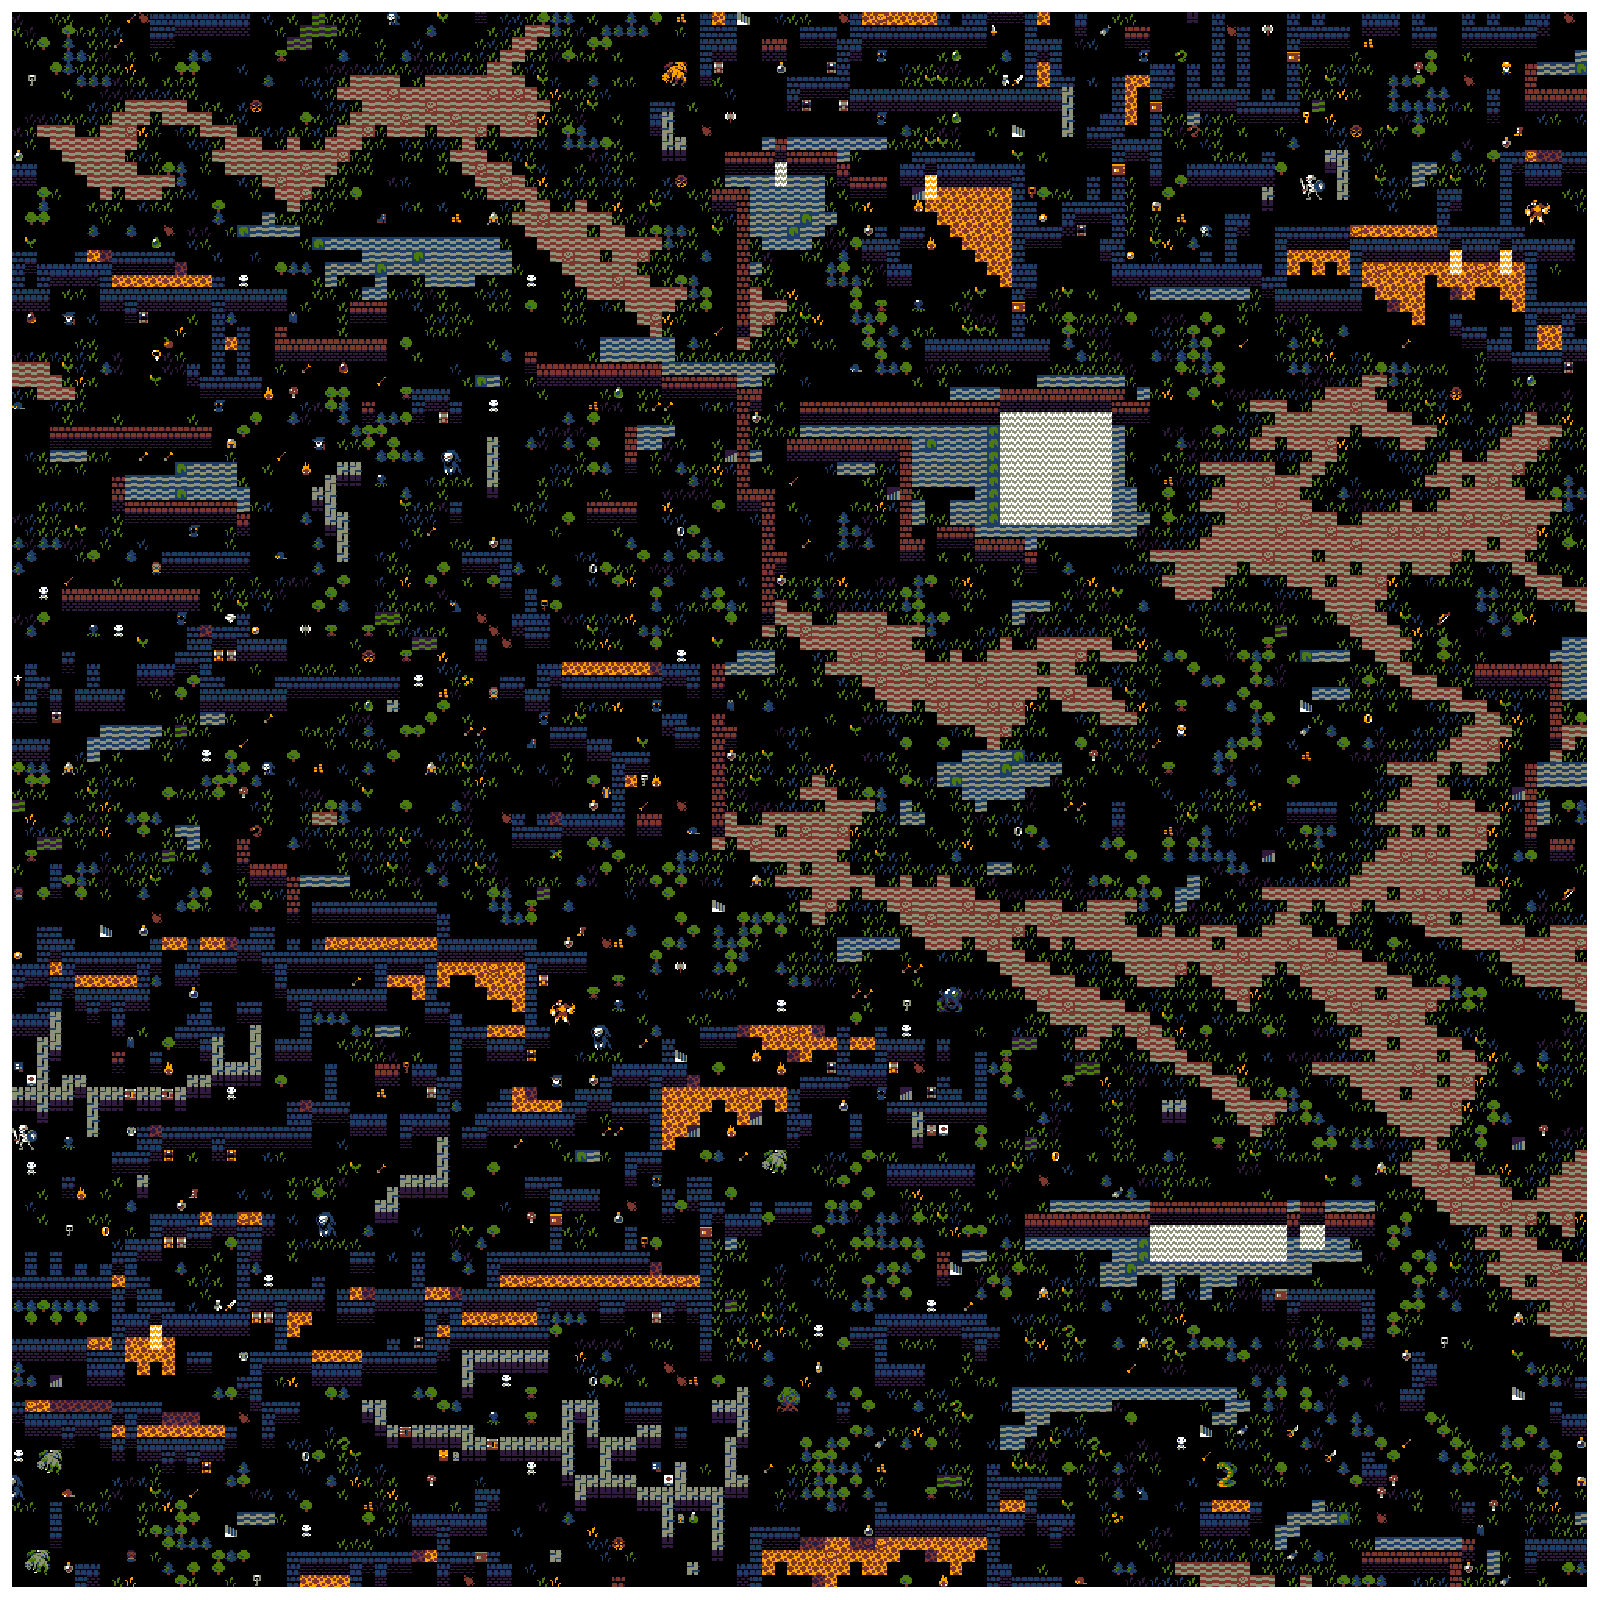
\includegraphics[width=0.7\textwidth]{img/minirogue_128x128.pdf}
%    \end{frame}
%  \end{centering}

%  \begin{frame}[fragile]{Introduction}
%    %Constraint Based Tiling Generation (\textit{CBTG})
%    \begin{columns}[T,onlytextwidth]
%      \column{0.5\textwidth}
%        \begin{block}{Definitions}
%          \begin{itemize}
%            \item \textit{Grid} composed of \textit{cells}
%            \item Each \textit{cell} can hold $D$ \textit{tiles}
%            \item Pairwise tile \textit{constraints} in each dimension ($\pm X, \pm Y, \pm Z$)
%          \end{itemize}
%        \end{block}
%      \column{0.5\textwidth}
%        \begin{block}{Example}
%          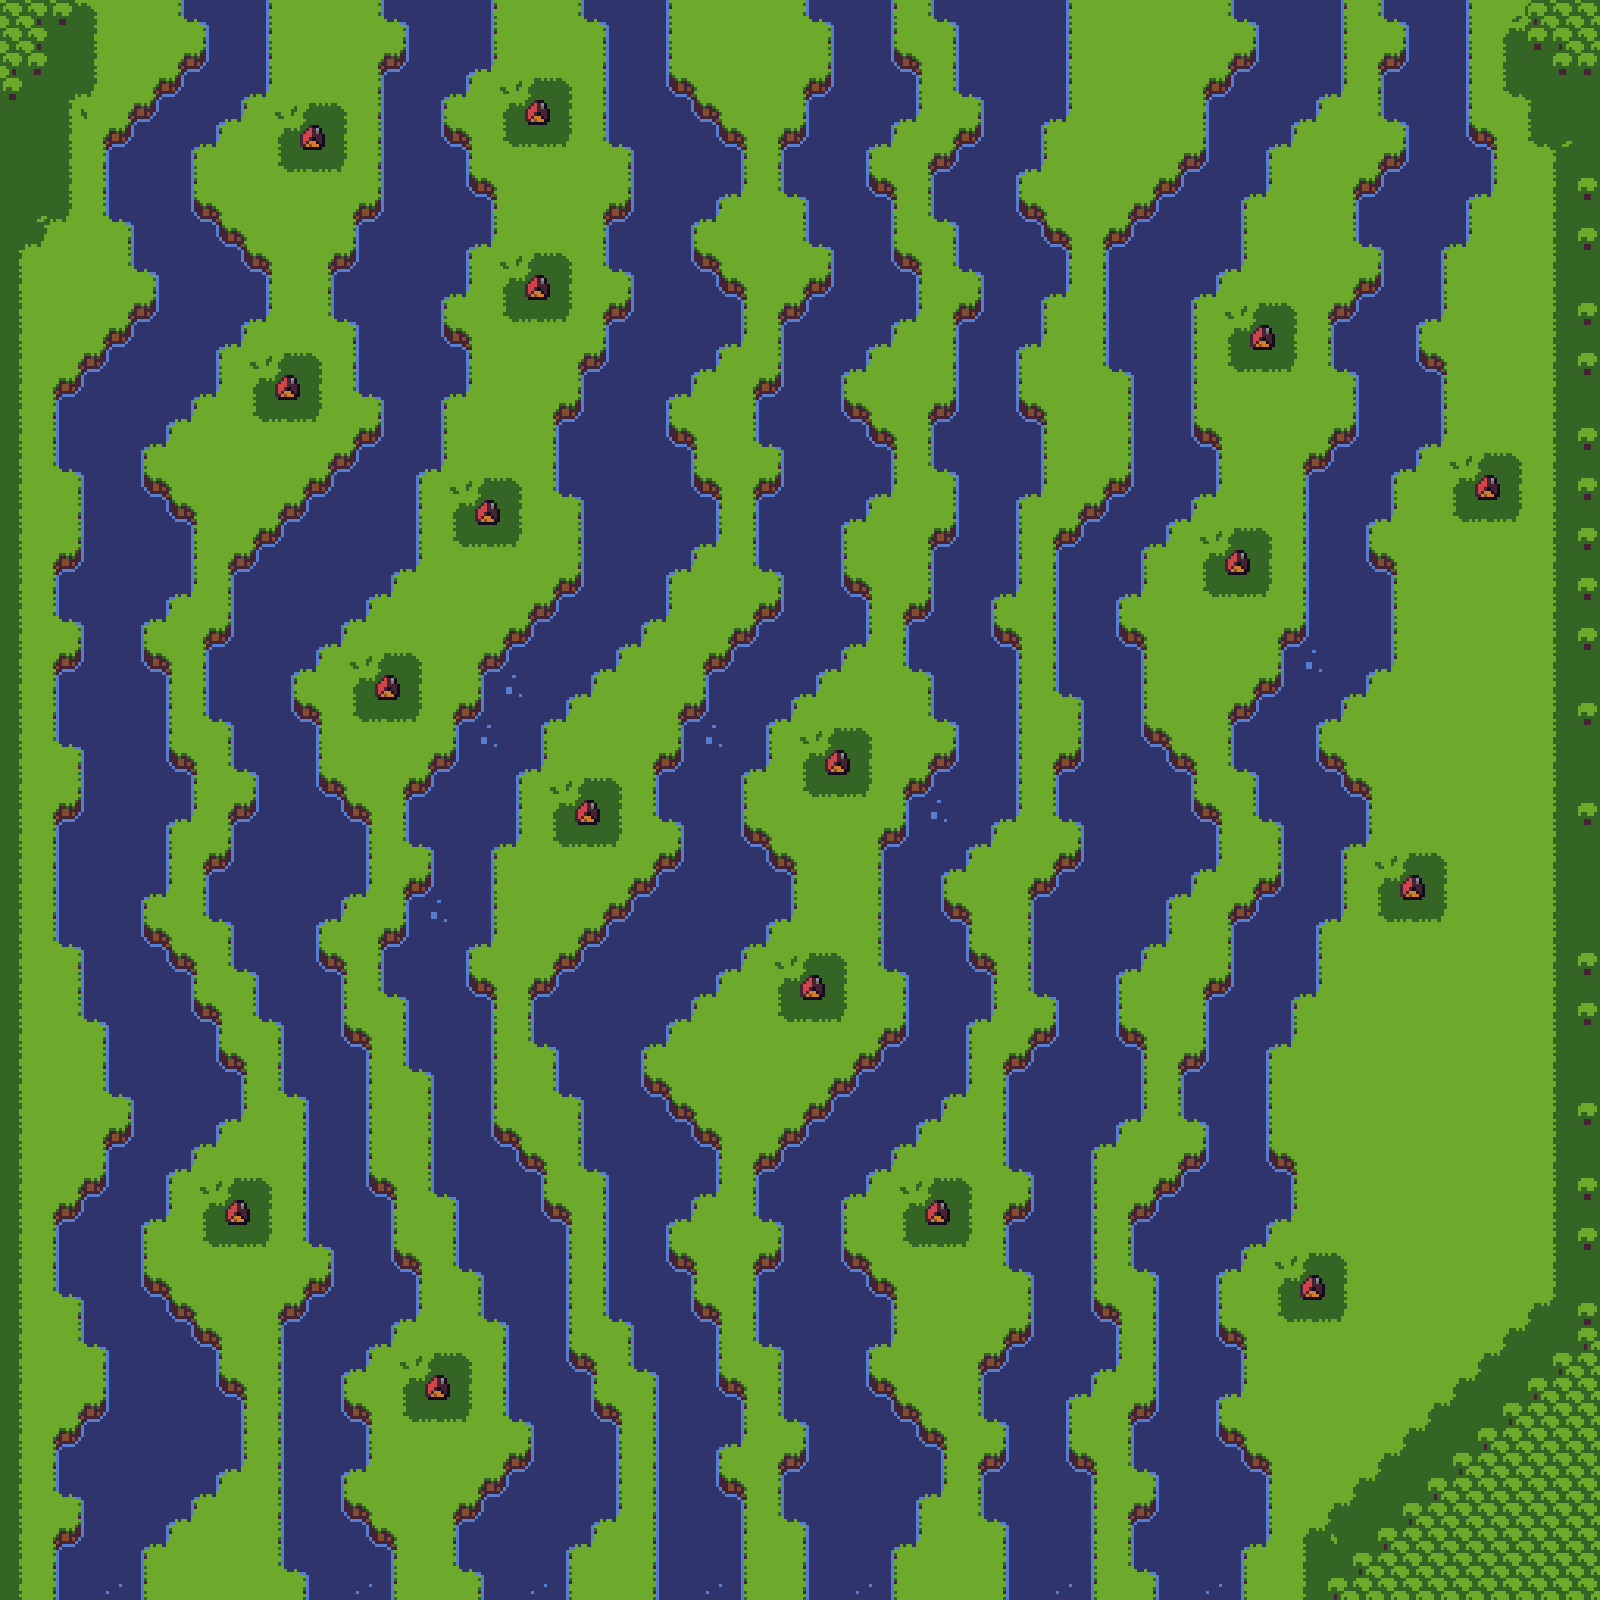
\includegraphics[width=0.9\textwidth]{img/forestmicro_64x64.pdf}
%        \end{block}
%    \end{columns}
%  \end{frame}

  \begin{frame}[fragile]{Introduction}
    Constraint Based Tiling Generation (\textit{CBTG}) Problem
    \begin{columns}[T,onlytextwidth]
      \column{0.5\textwidth}
        \begin{block}{}
          \hfill \\
          \textbf{Find a valid grid realization}
          \hfill \\
          \hfill \\
          A \textit{realization} is a single \textit{tile} placement at each \textit{cell} \\
          respecting \textit{constraints}.
          \hfill \\
          \hfill \\
          (\textit{Cell} can hold up to $D$ \textit{tiles})

          %\begin{itemize}
          %  \item A \textit{realization} is a single \textit{tile} placement at each \textit{cell} respecting \textit{constraints}.
          %  \item A \textit{contradiction} if no tiles left at a cell location
          %\end{itemize}
        \end{block}
      \column{0.5\textwidth}
        \begin{block}{Example}
          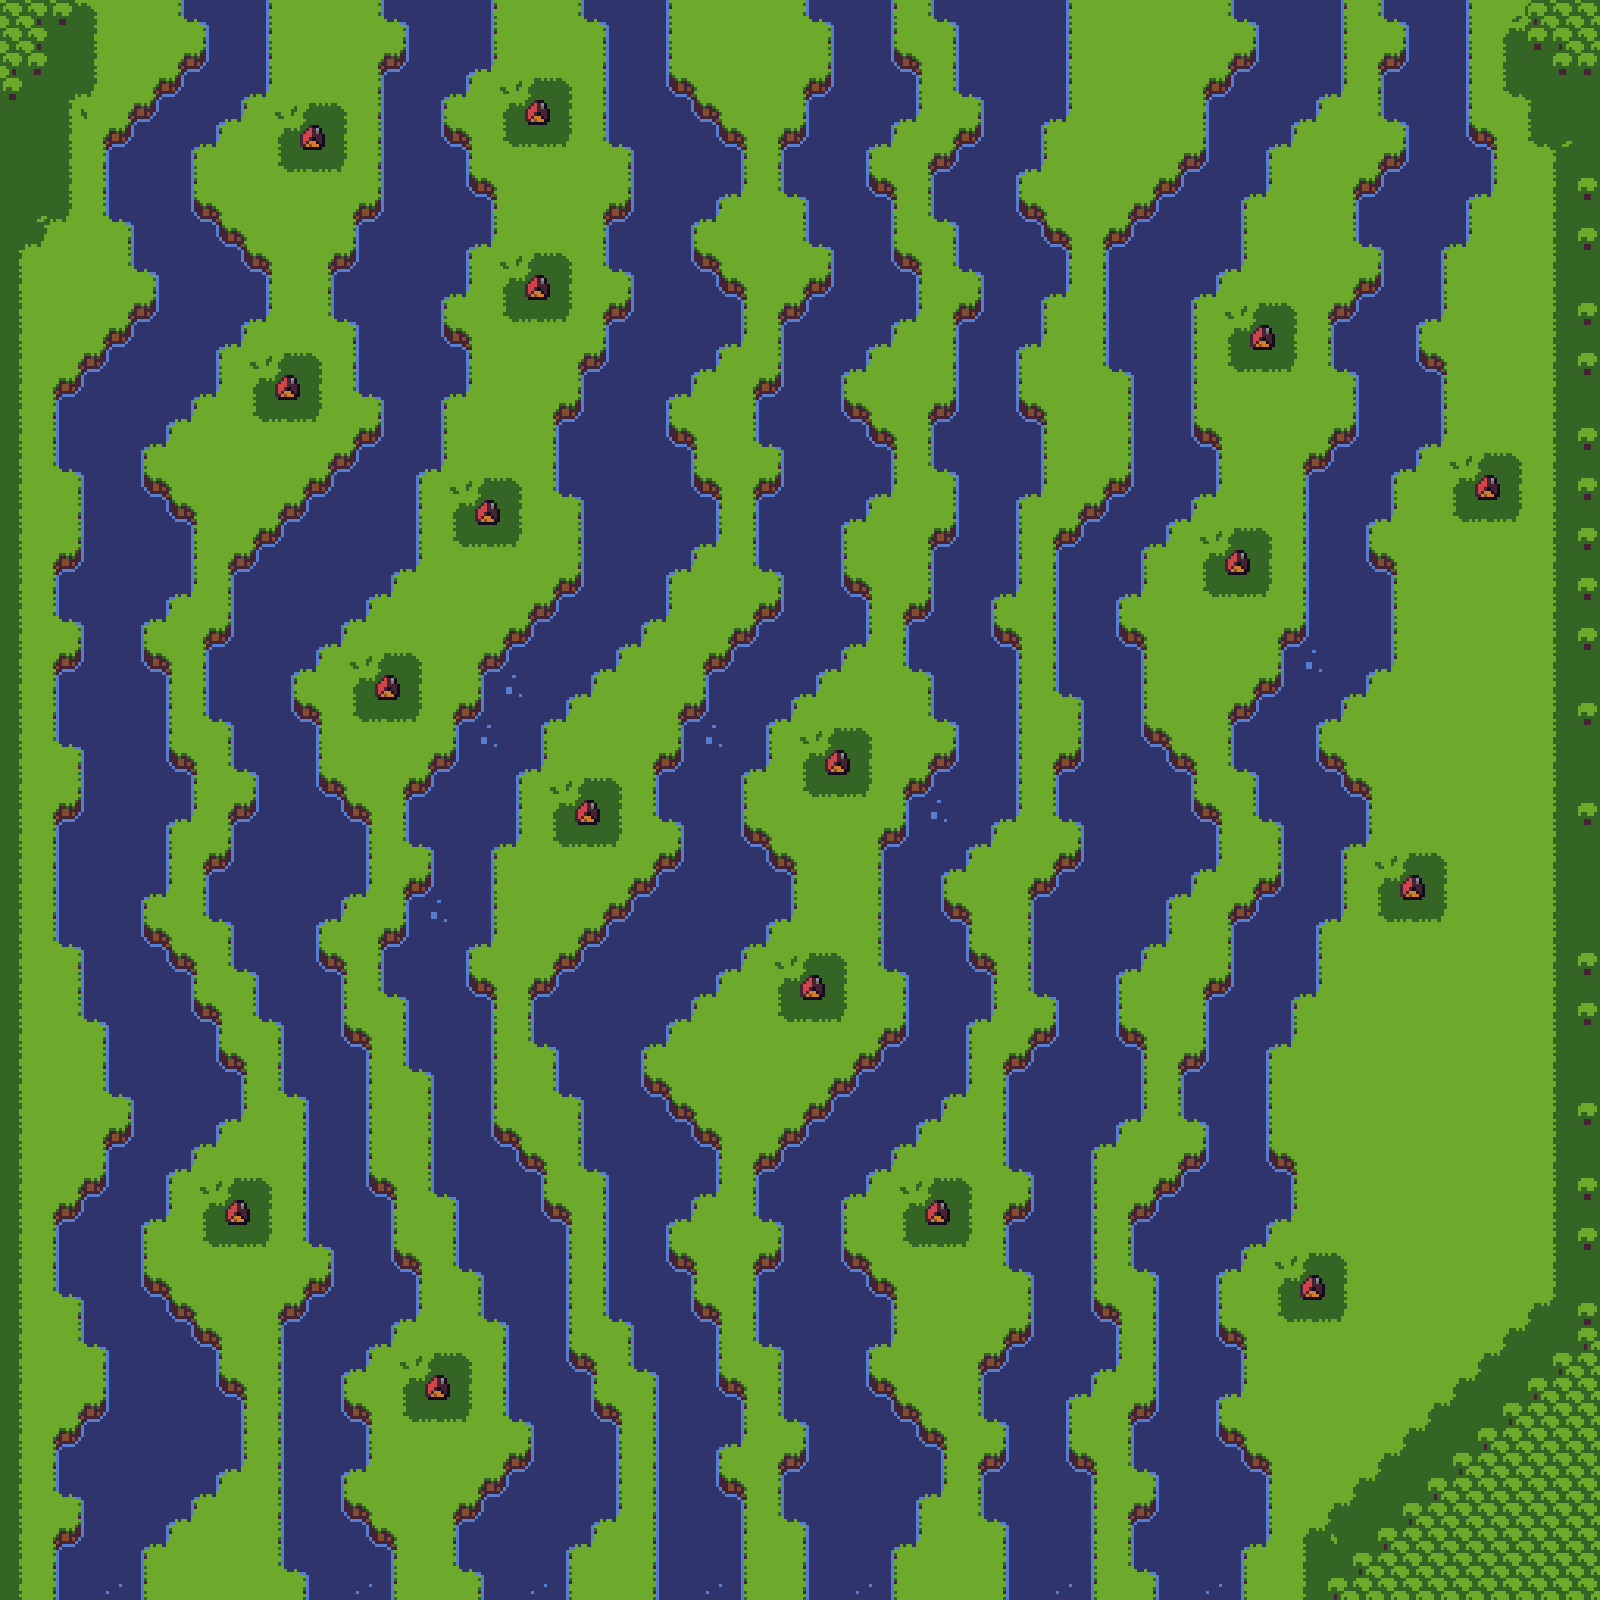
\includegraphics[width=0.9\textwidth]{img/forestmicro_64x64.pdf}
        \end{block}
    \end{columns}
  \end{frame}

  \begin{frame}[fragile]{Introduction}
    A region is \textit{Arc Consistent} if all \textit{tiles} in every \textit{cell} within the region have at least
    one valid neighbor in each direction
    \hfill \\
    \hfill \\
    The basis for a \textit{Constraint Propagation} algorithm
    can be made by removing tiles without a valid neighbor
    \hfill \\
    \hfill \\
    \textit{Block Level Solver}: completely maintains \textit{Arc Consistency}
    \hfill \\
    \hfill \\
    \textit{Grid Level Solver}: only keep minimal information for the entire grid but
        work on \textit{block} sub-regions

  \end{frame}


%  \begin{frame}[fragile]{Introduction}
%    \begin{columns}[T,onlytextwidth]
%      \column{0.5\textwidth}
%        \begin{block}{Definitions}
%          \hfill \\
%
%          A region is \textit{Arc Consistent} if all \textit{tiles} in every \textit{cell} within the region have at least
%          one valid neighbor in each direction
%
%%          \begin{itemize}
%%            \item A tile has \textit{support} if \\
%%              there's a valid neighbor
%%              in each
%%              grid dimension direction
%%            \item A region is \textit{Arc Consistent} \\ if all \textit{tiles} within the region are \textit{supported}
%%          \end{itemize}
%
%        \end{block}
%      \column{0.5\textwidth}
%        \begin{block}{Example}
%          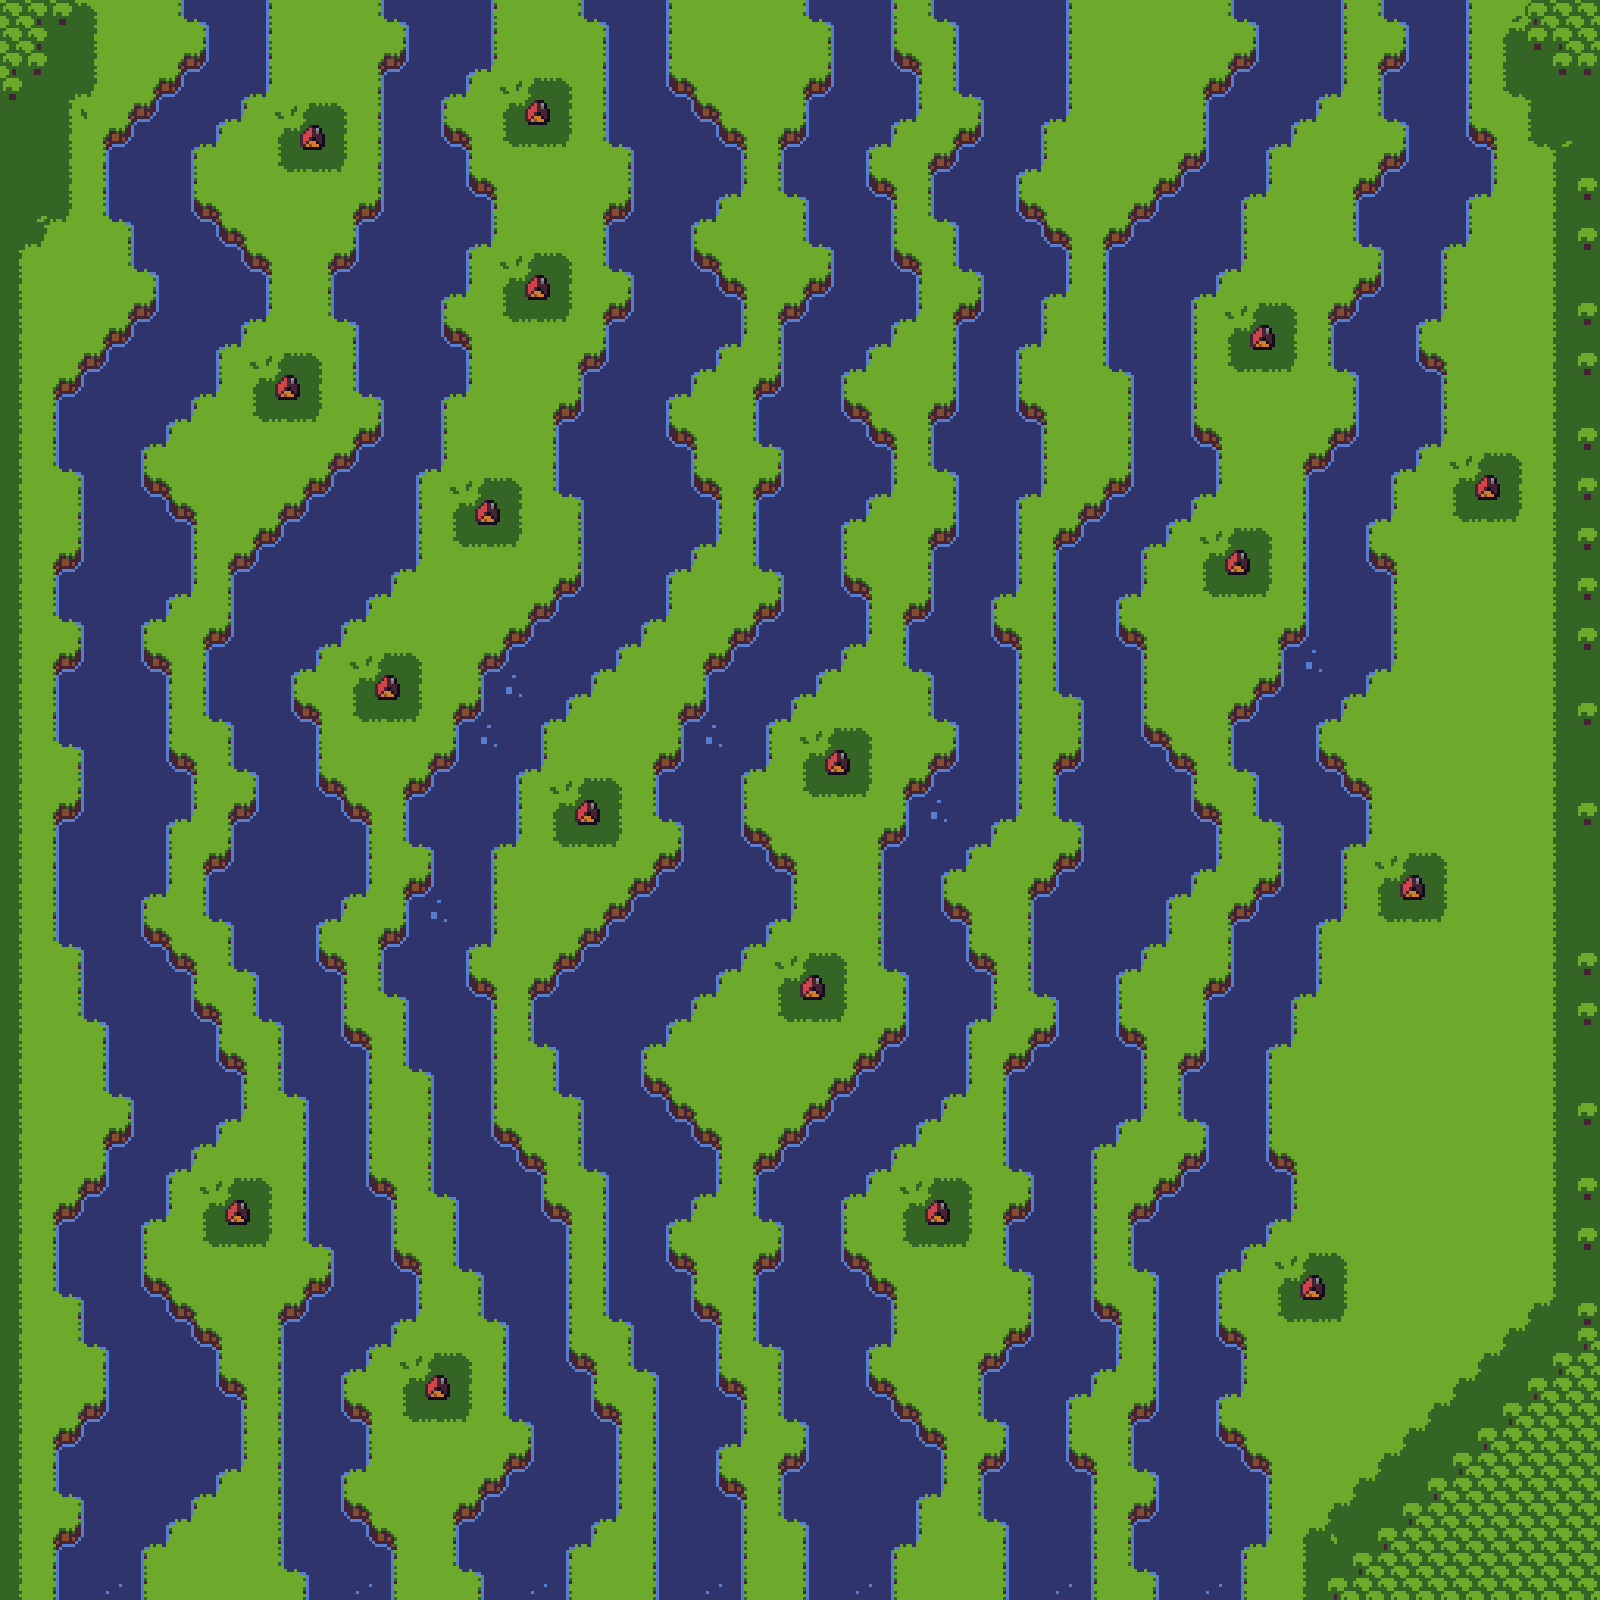
\includegraphics[width=0.9\textwidth]{img/forestmicro_64x64.pdf}
%        \end{block}
%    \end{columns}
%  \end{frame}


%  \begin{frame}[fragile]{Introduction}
%    \begin{columns}[T,onlytextwidth]
%      \column{0.5\textwidth}
%        \begin{block}{Definitions}
%          \hfill \\
%          The basis for a \textit{Constraint Propagation} algorithm
%          can be made by removing tiles without \\
%          a valid neighbor
%        \end{block}
%      \column{0.5\textwidth}
%        \begin{block}{Example}
%          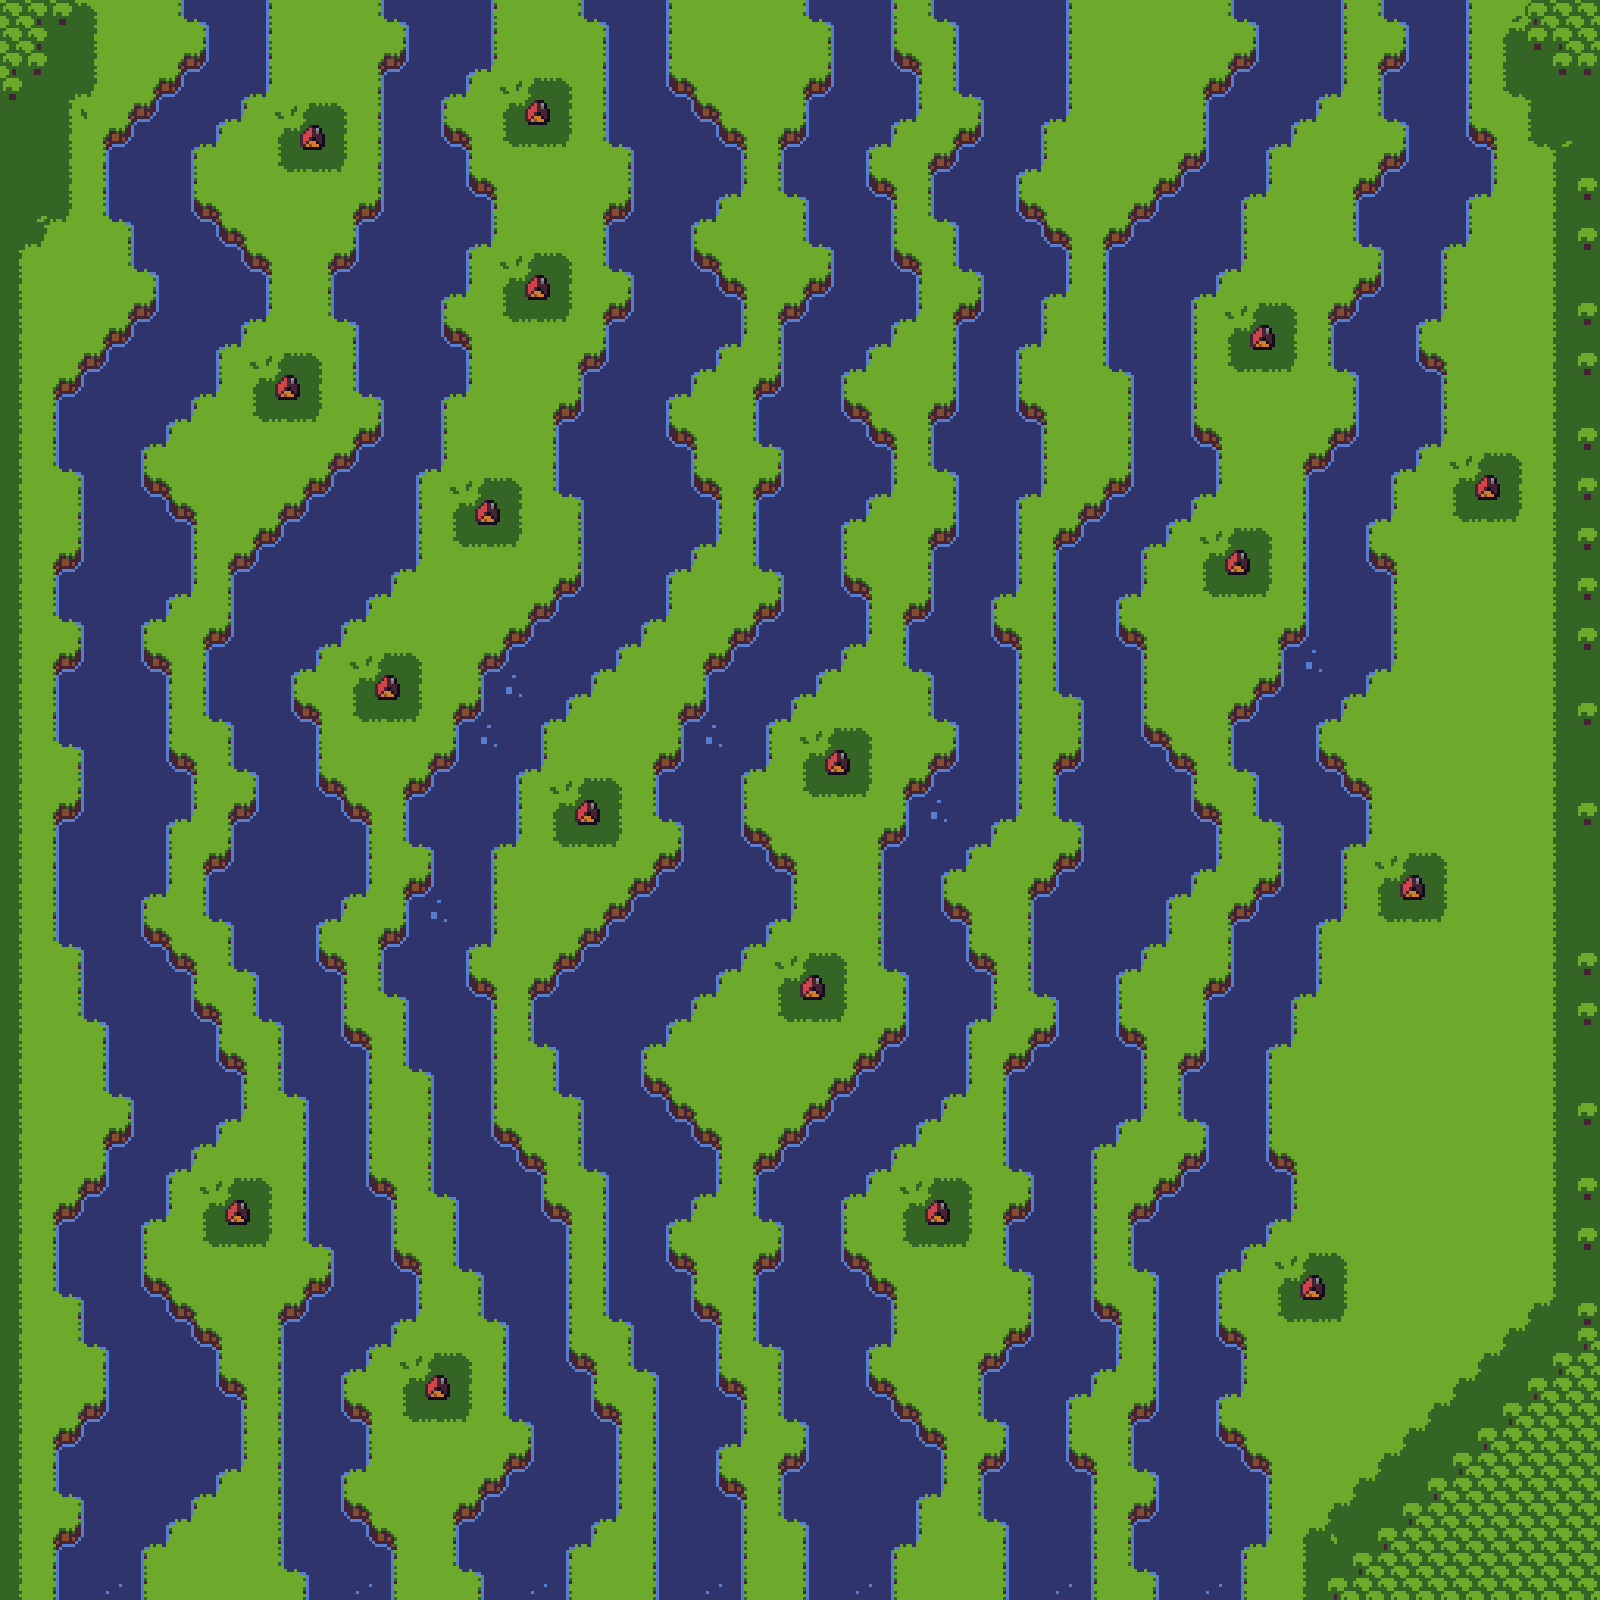
\includegraphics[width=0.9\textwidth]{img/forestmicro_64x64.pdf}
%        \end{block}
%    \end{columns}
%  \end{frame}


%  \begin{frame}[fragile]{Introduction}
%    \begin{columns}[T,onlytextwidth]
%      \column{0.5\textwidth}
%        \begin{block}{Definitions}
%          \hfill \\
%          One such algorithm is \textit{AC4}, which maintains a data
%          structure to count the \textit{support} of each \textit{tile}
%          in each dimension direction
%        \end{block}
%      \column{0.5\textwidth}
%        \begin{block}{Example}
%          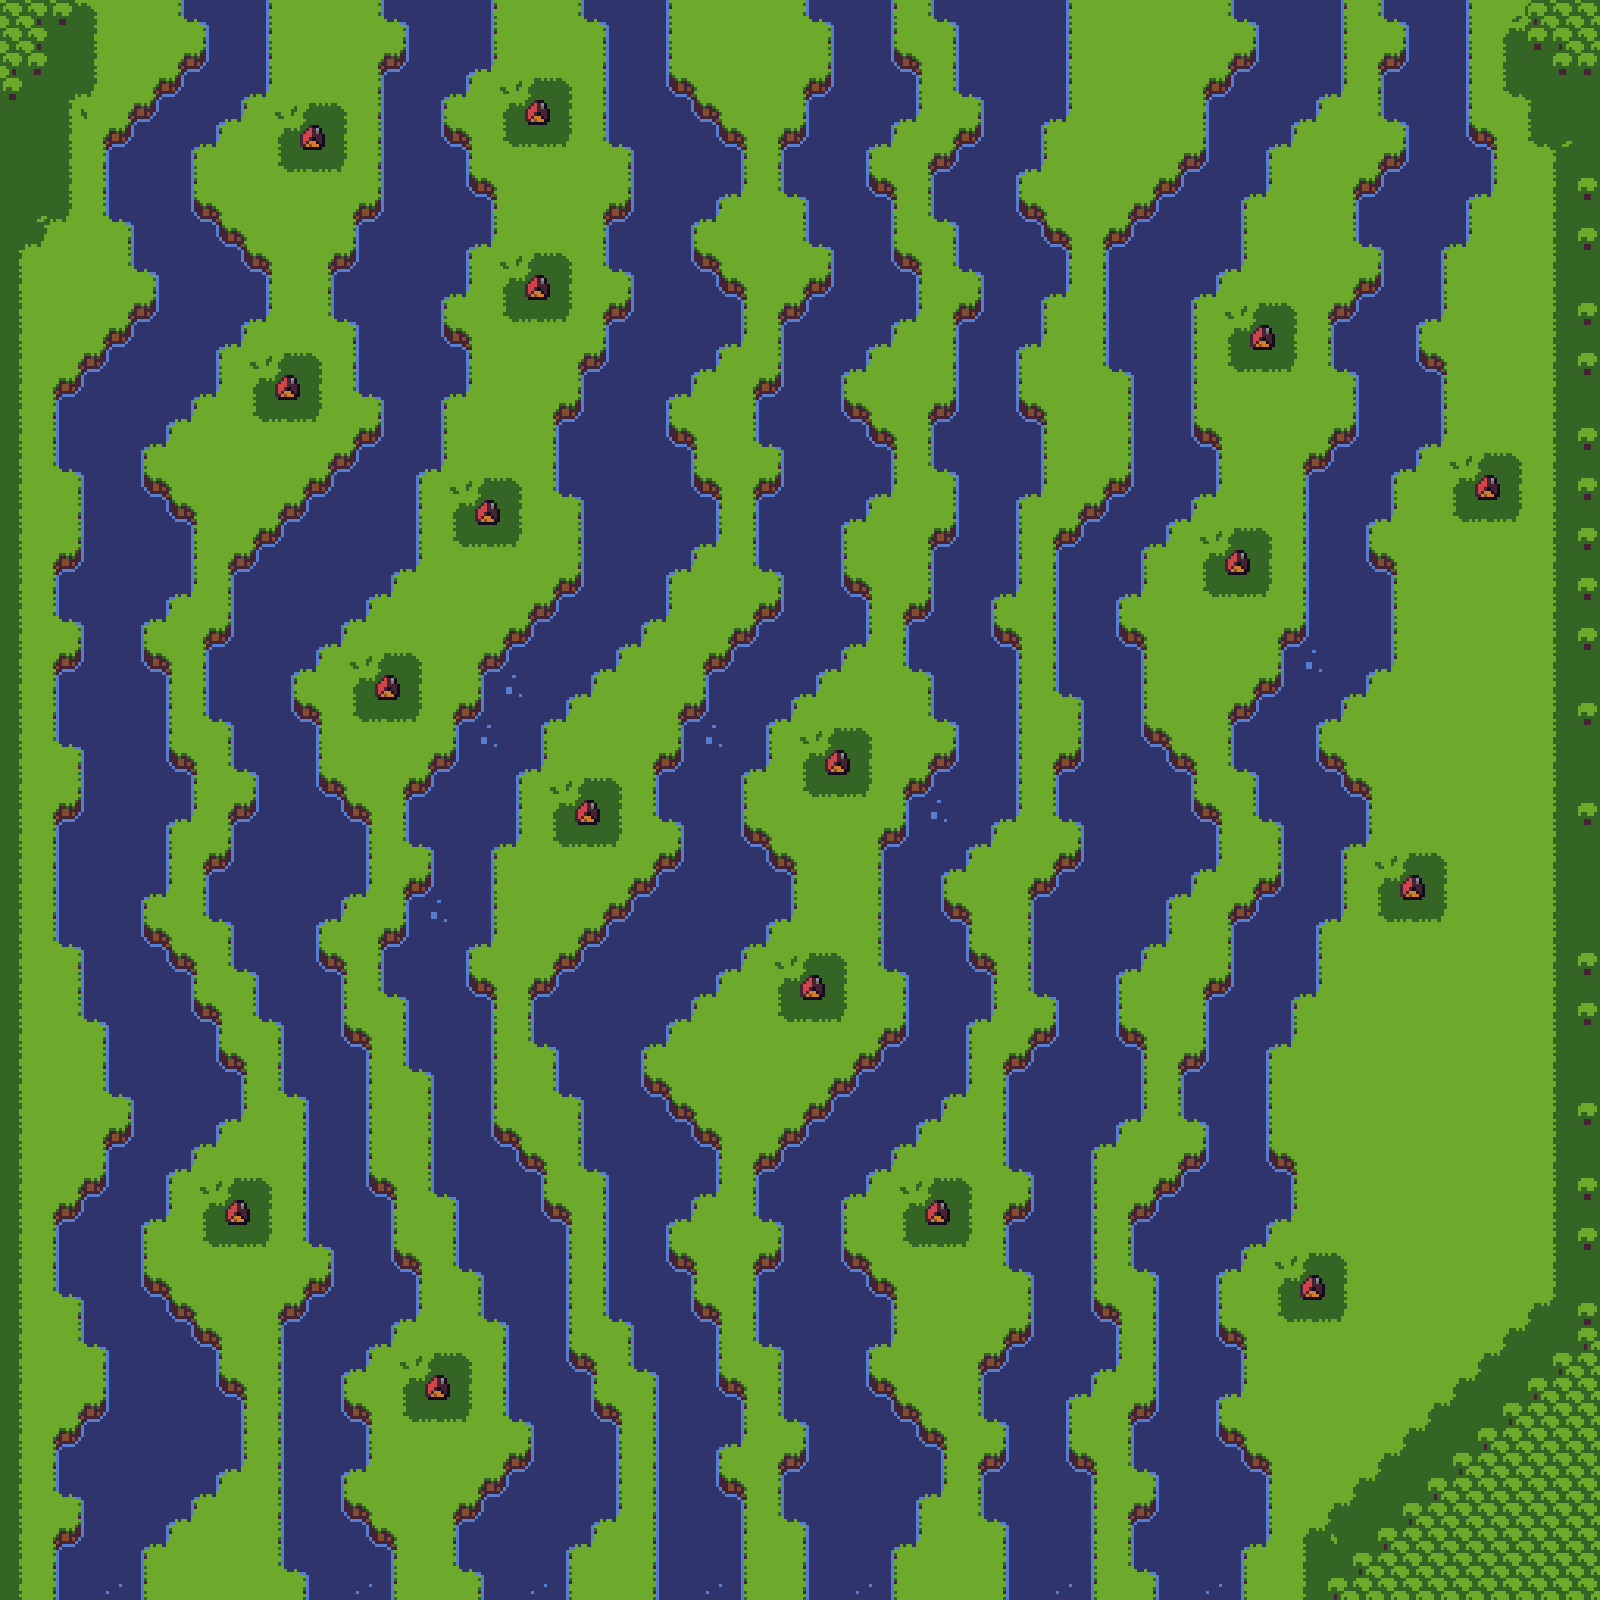
\includegraphics[width=0.9\textwidth]{img/forestmicro_64x64.pdf}
%        \end{block}
%    \end{columns}
%  \end{frame}

%  \begin{frame}[fragile]{Introduction}
%    %\textit{Block} and \textit{Grid} level solvers
%    \begin{columns}[T,onlytextwidth]
%      \column{0.5\textwidth}
%        \begin{block}{Definitions}
%          \hfill \\
%          \begin{itemize}
%            \item \textit{Block Level Solver}: \\
%              completely maintains \textit{Arc Consistency}
%          \end{itemize}
%        \end{block}
%      \column{0.5\textwidth}
%        \begin{block}{Example}
%          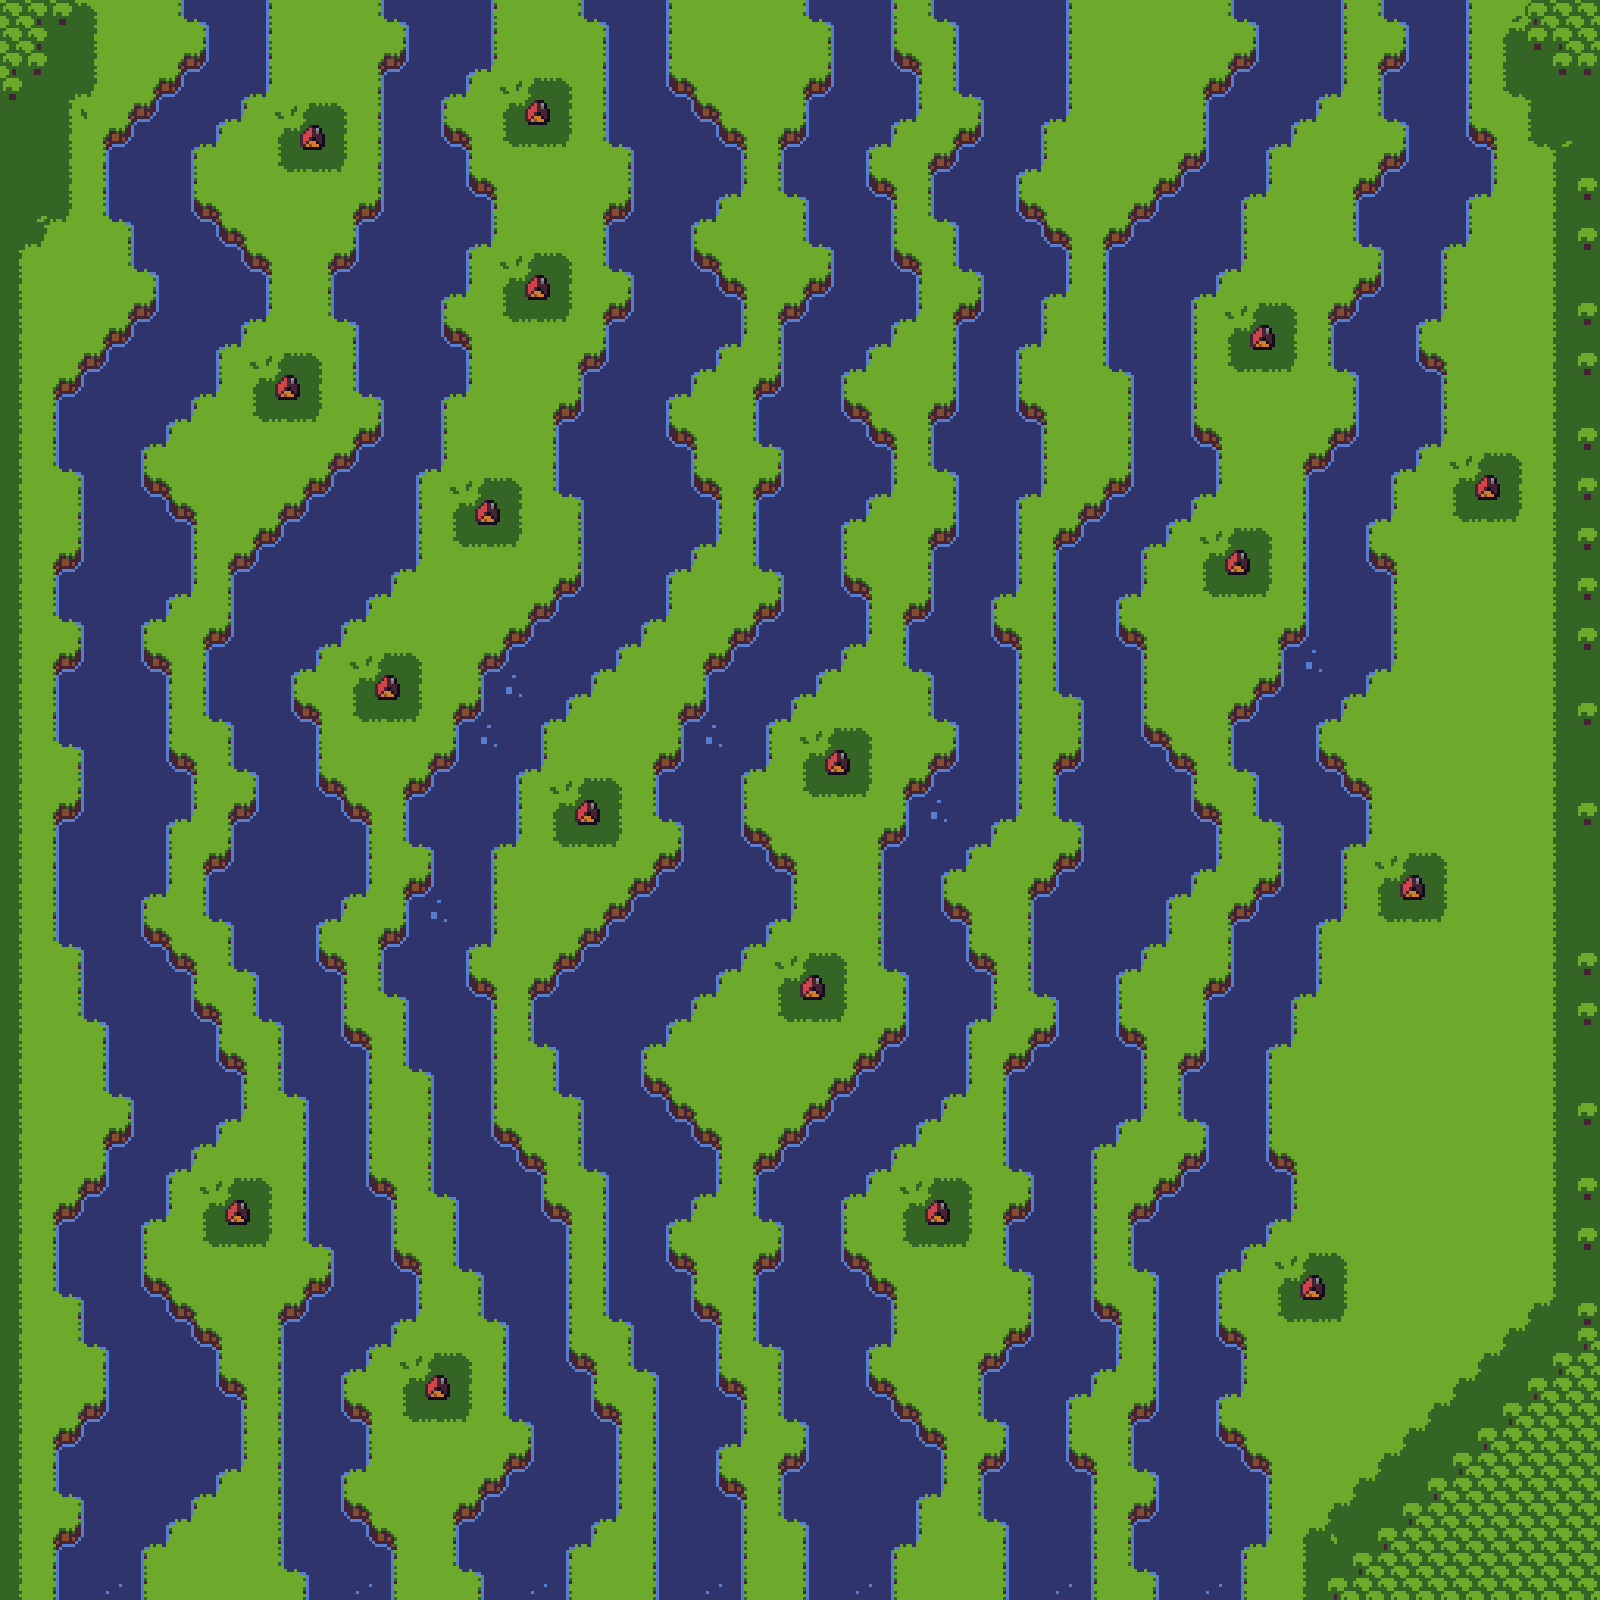
\includegraphics[width=0.9\textwidth]{img/forestmicro_64x64.pdf}
%        \end{block}
%    \end{columns}
%  \end{frame}

%  \begin{frame}[fragile]{Introduction}
%    %\textit{Block} and \textit{Grid} level solvers
%    \begin{columns}[T,onlytextwidth]
%      \column{0.5\textwidth}
%        \begin{block}{Definitions}
%          \hfill \\
%          \begin{itemize}
%            \item \textit{Block Level Solver}: \\
%              completely maintains \textit{Arc Consistency}
%            \item \textit{Grid Level Solver}: \\
%              only keep minimal information for the entire grid but
%              work on \textit{block} sub-regions
%          \end{itemize}
%        \end{block}
%      \column{0.5\textwidth}
%        \begin{block}{Example}
%          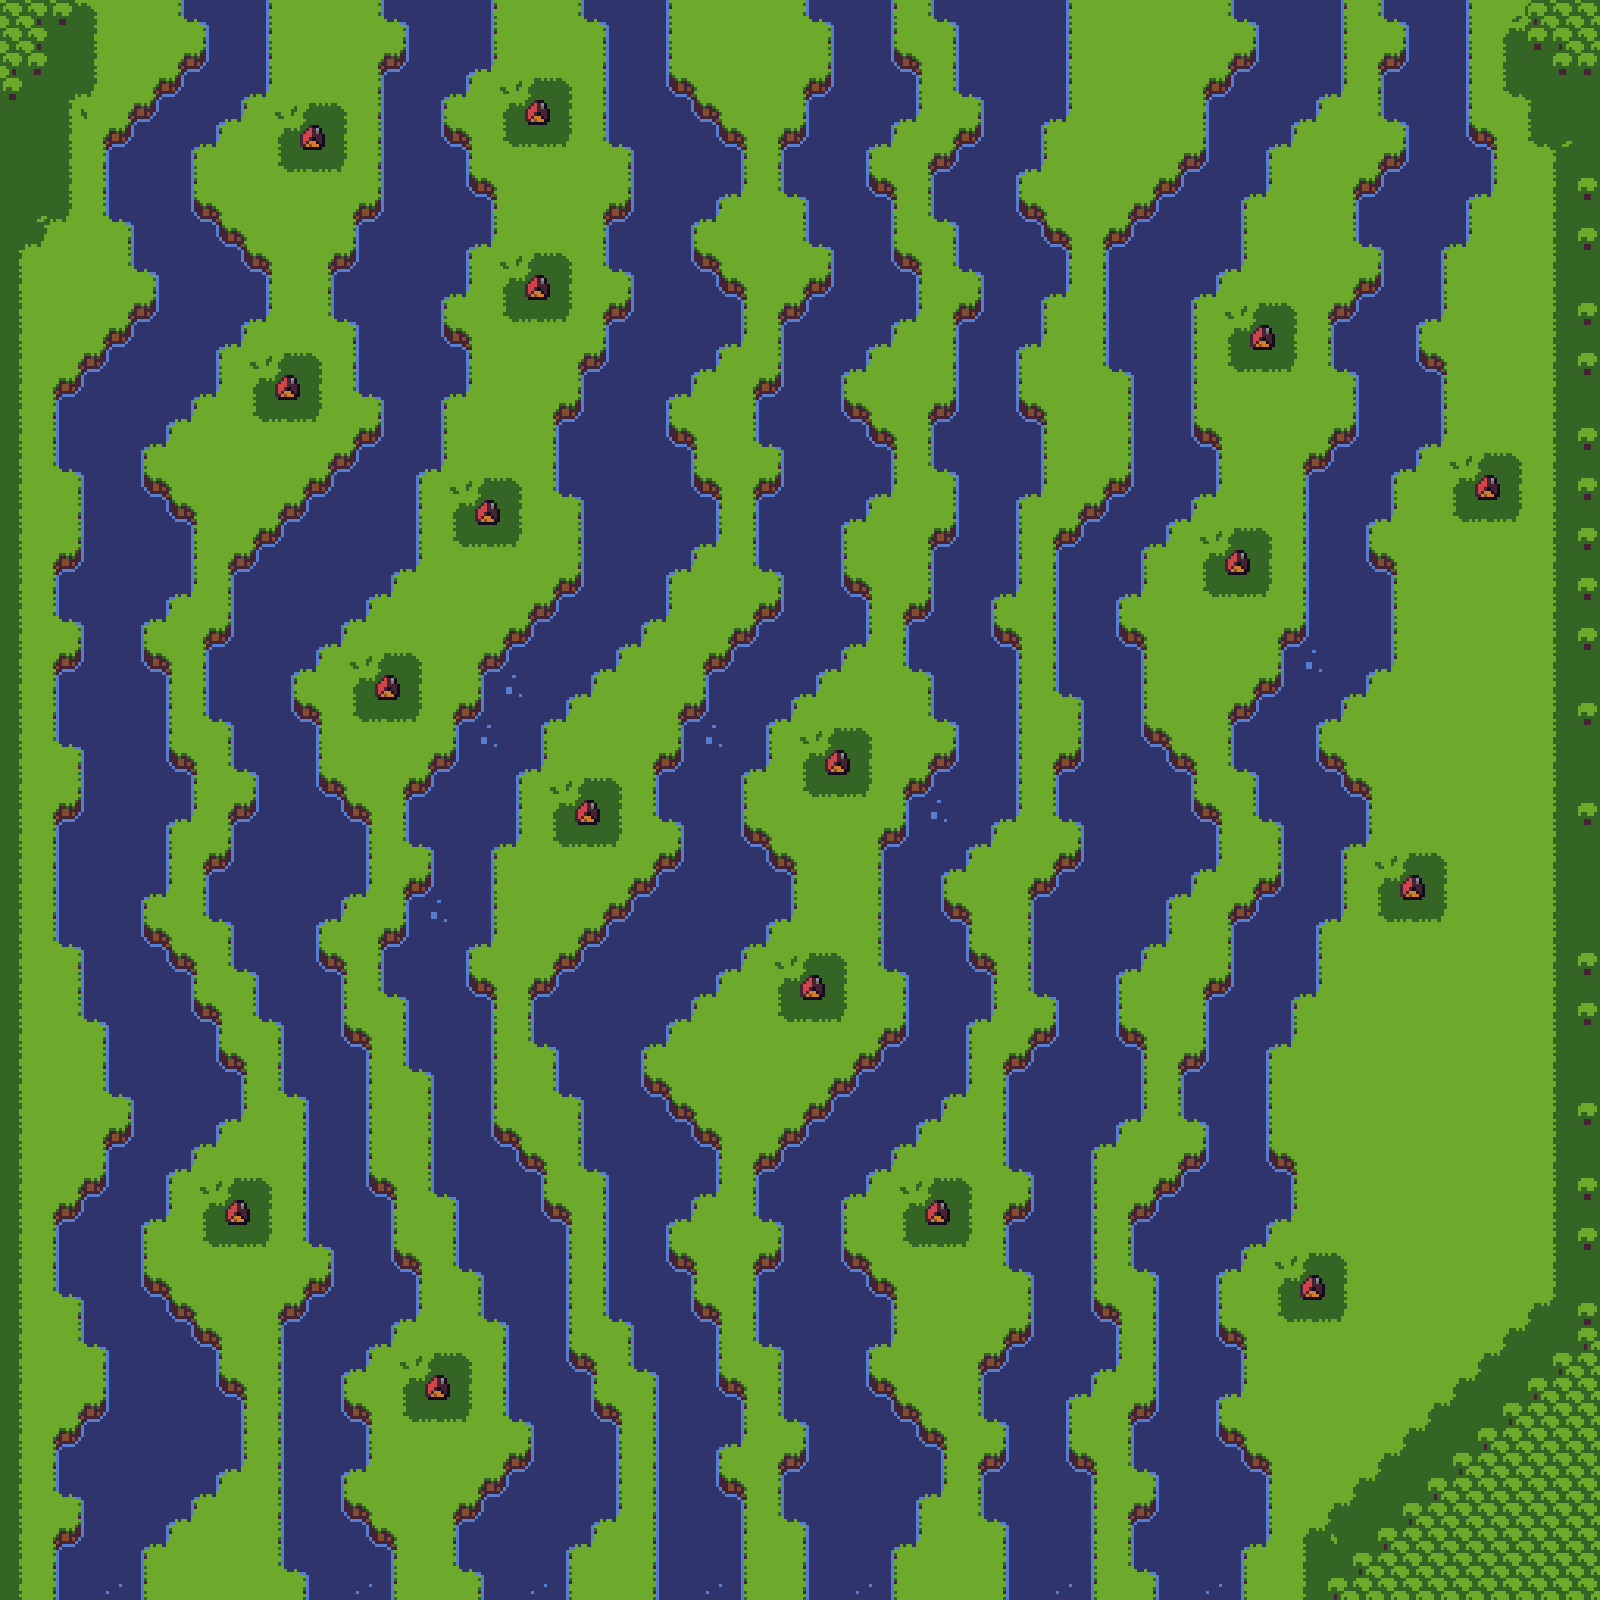
\includegraphics[width=0.9\textwidth]{img/forestmicro_64x64.pdf}
%        \end{block}
%    \end{columns}
%  \end{frame}


  %%%%%%%%%%%%%%
  %%%%%%%%%%%%%%
  %%%%%%%%%%%%%%
  
  % summary_related_work

  \begin{frame}[fragile]{Related Work}

\begin{table}[h]
  \centering
  \begin{tabular}[t]{l|cccc}
      & \textit{WFC} & \textit{BMS} & \textit{MMS} & \textit{POMS} \\
    \hline
    \specialcellCenter{Solver Type} & Block & Block & Grid & \textbf{Grid} \\
    \specialcellCenter{Contradiction \\ \ \ Resilience} & No & Yes & Yes & \textbf{Yes} \\
    \specialcellCenter{Block Step \ \ \ \ \\ \ \ \ \ Consistent} & n/a & n/a & Yes & \textit{\textbf{No}} \\
    \specialcellCenter{Indeterminate \\ \ \ Initial State} & Yes & Yes & No & \textbf{Yes} \\
    \specialcellCenter{Ergodic} & Yes & Yes & No & \textbf{Yes} \\
    \hline
  \end{tabular}

  $\begin{array}{l}
  \textit{WFC}: Wave Function Collapse (Gumin) \\
  \textit{BMS}: Breakout Model Synthesis (Hoetzlein) \\
  \textit{MMS}: Modify in Blocks Model Synthesis (Merrell) \\
  \textit{POMS}: Punch Out Model Synthesis \\
  \end{array}$

\end{table}

  \end{frame}

  %%
  %% tile_influence

  \begin{frame}[fragile]{Related Work}
    \textit{Tile Arc Consistent Correlation Length} (\textit{TACCL}) (Hoetzlein) \\
    \hfill \\
    How much influence does a tile choice have over long distances? \\
    \hfill \\
    TACCL as a heuristic to estimate correlation length
  \end{frame}

  %%

  \begin{frame}[fragile]{Related Work}
    \textit{Tile Arc Consistent Correlation Length} (\textit{TACCL})
    \begin{columns}[T,onlytextwidth]
      \column{0.5\textwidth}
        \begin{block}{TACCL}
          \hfill \\
          Take block in isolation
          \begin{itemize}
            \item Set block to indeterminate state
            \item Fix a tile at the center
            \item Propagate constraints
            \item Take minimum bounding box of altered cells
            \item Repeat for all tiles
          \end{itemize}
        \end{block}
      \column{0.5\textwidth}
        \begin{block}{Example}
          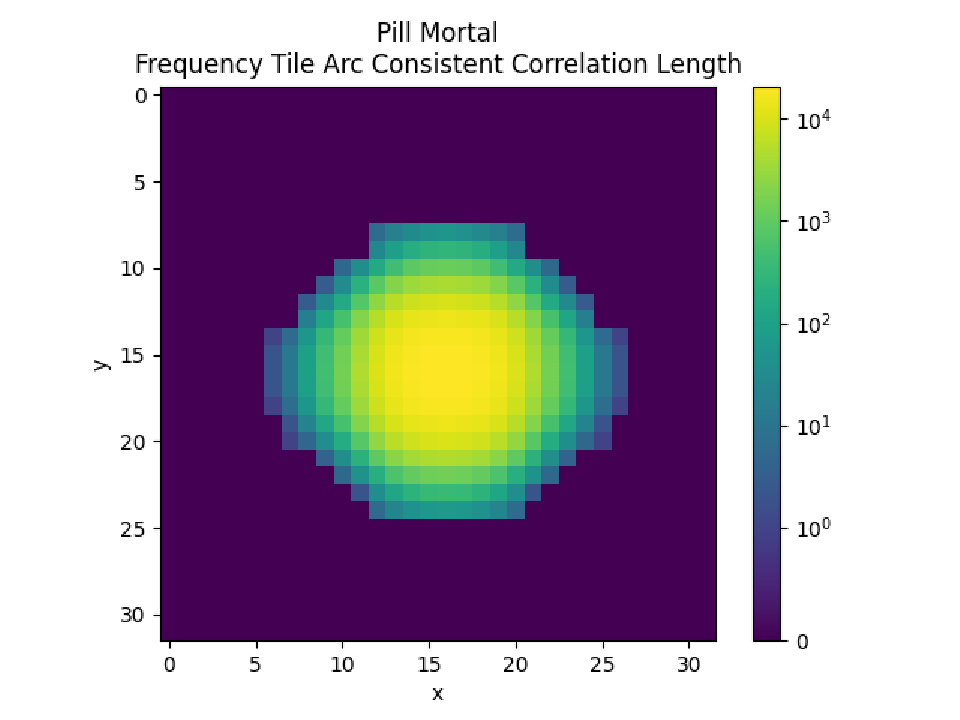
\includegraphics[width=1.125\textwidth]{img/pm_freq_taccl.pdf}
        \end{block}
    \end{columns}
  \end{frame}



  %%%%%%%%%%%%%%%
  %%%%%%%%%%%%%%%
  %%%%%%%%%%%%%%%
  %%%%%%%%%%%%%%%

  %\section{Algorithm}

  \begin{frame}[fragile]{Algorithm: Overview }
    \begin{figure}
      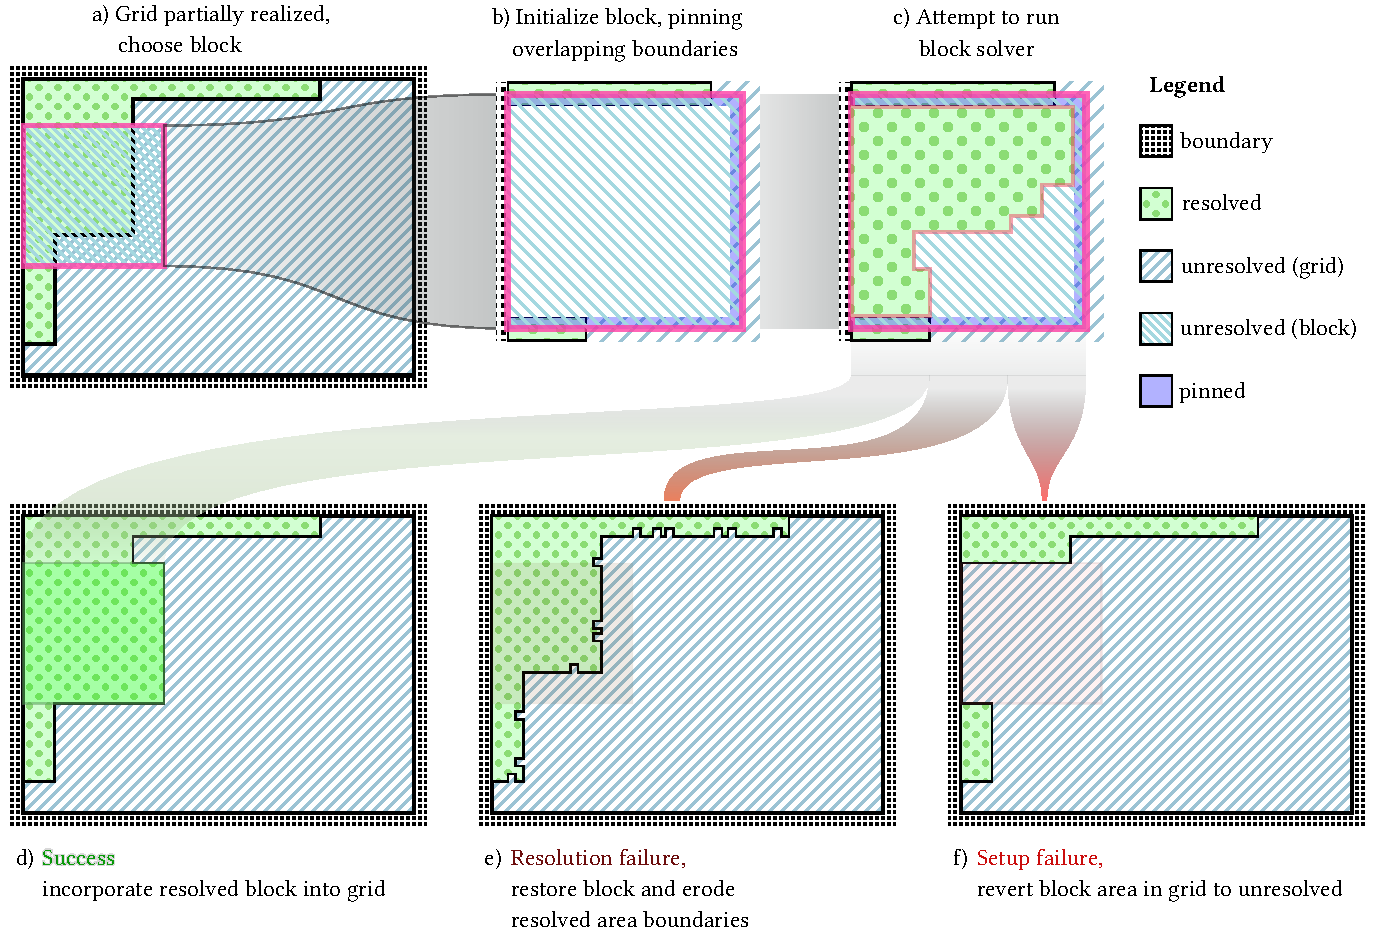
\includegraphics[width=\textwidth]{figs/poms_figalg.pdf}
    \end{figure}
  \end{frame}

  \begin{frame}[fragile]{Algorithm}
    \begin{figure}
      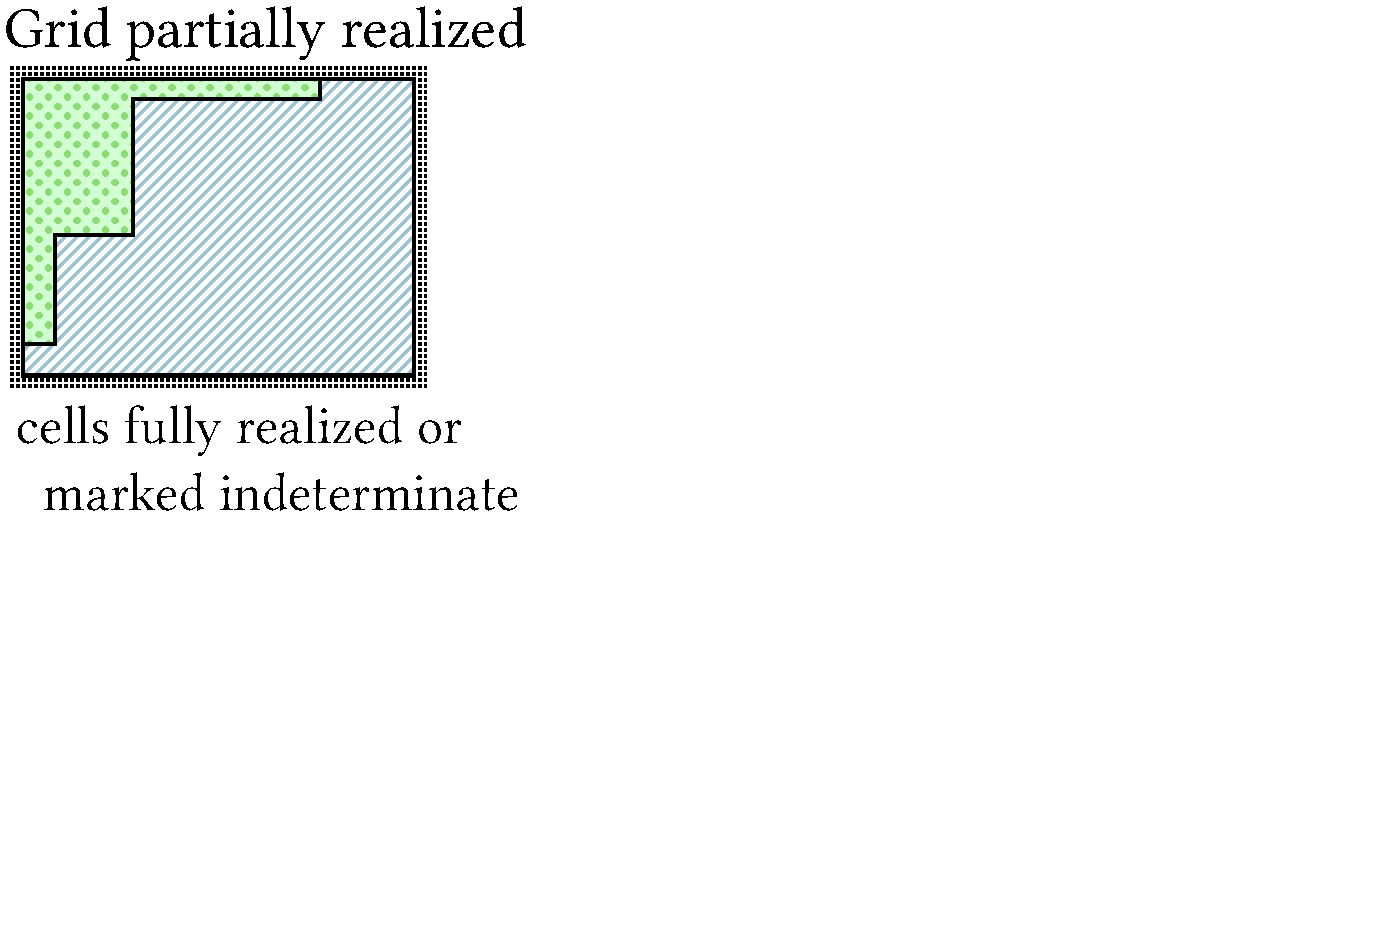
\includegraphics[width=\textwidth]{figs/poms_alg0.pdf}
    \end{figure}
  \end{frame}

  \begin{frame}[fragile]{Algorithm}
    \begin{figure}
      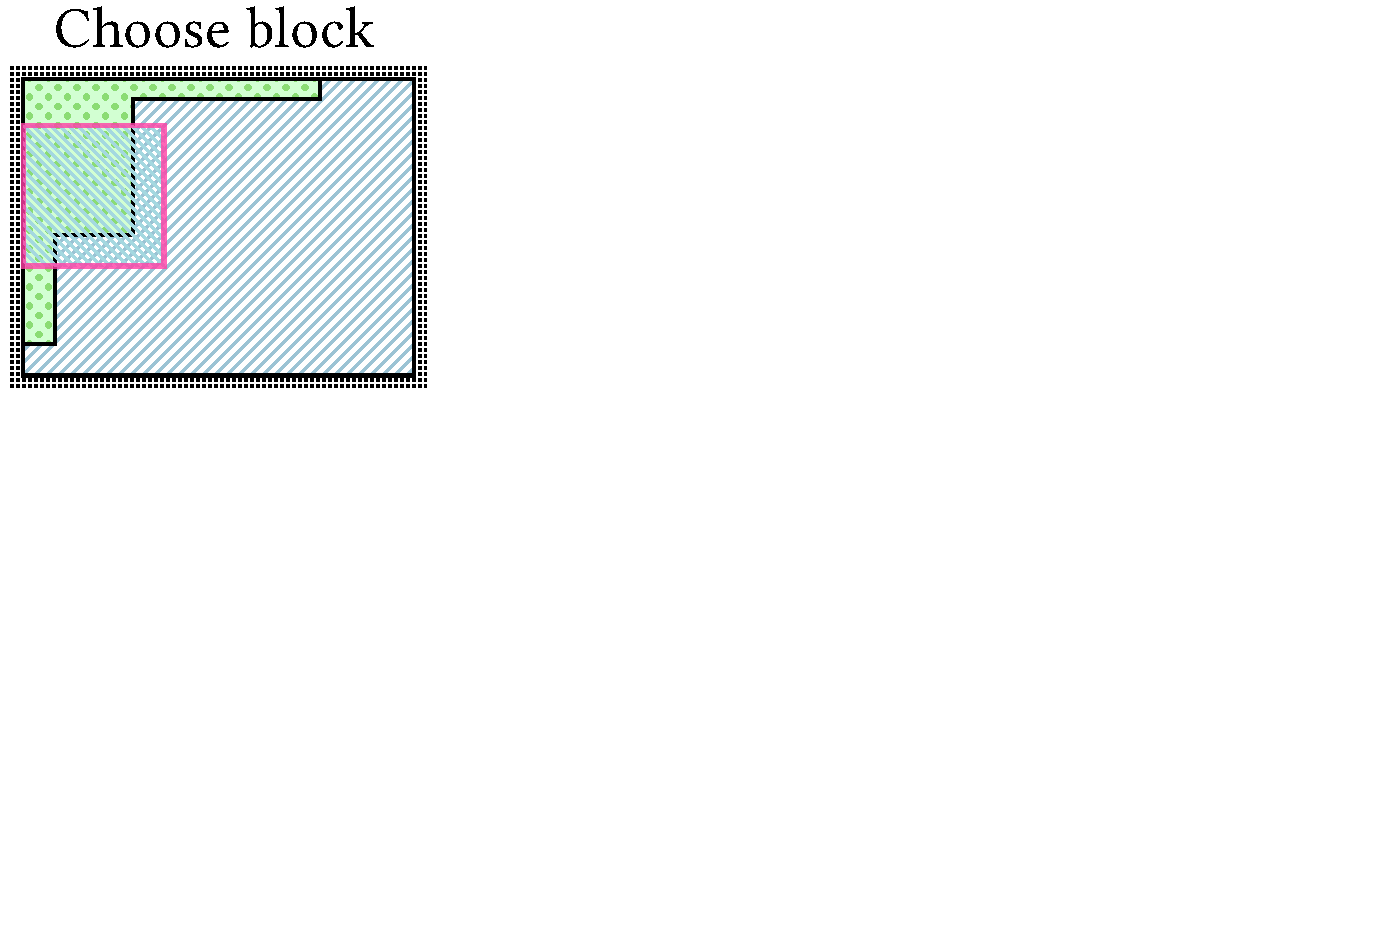
\includegraphics[width=\textwidth]{figs/poms_alg1.pdf}
    \end{figure}
  \end{frame}

  \begin{frame}[fragile]{Algorithm}
    \begin{figure}
      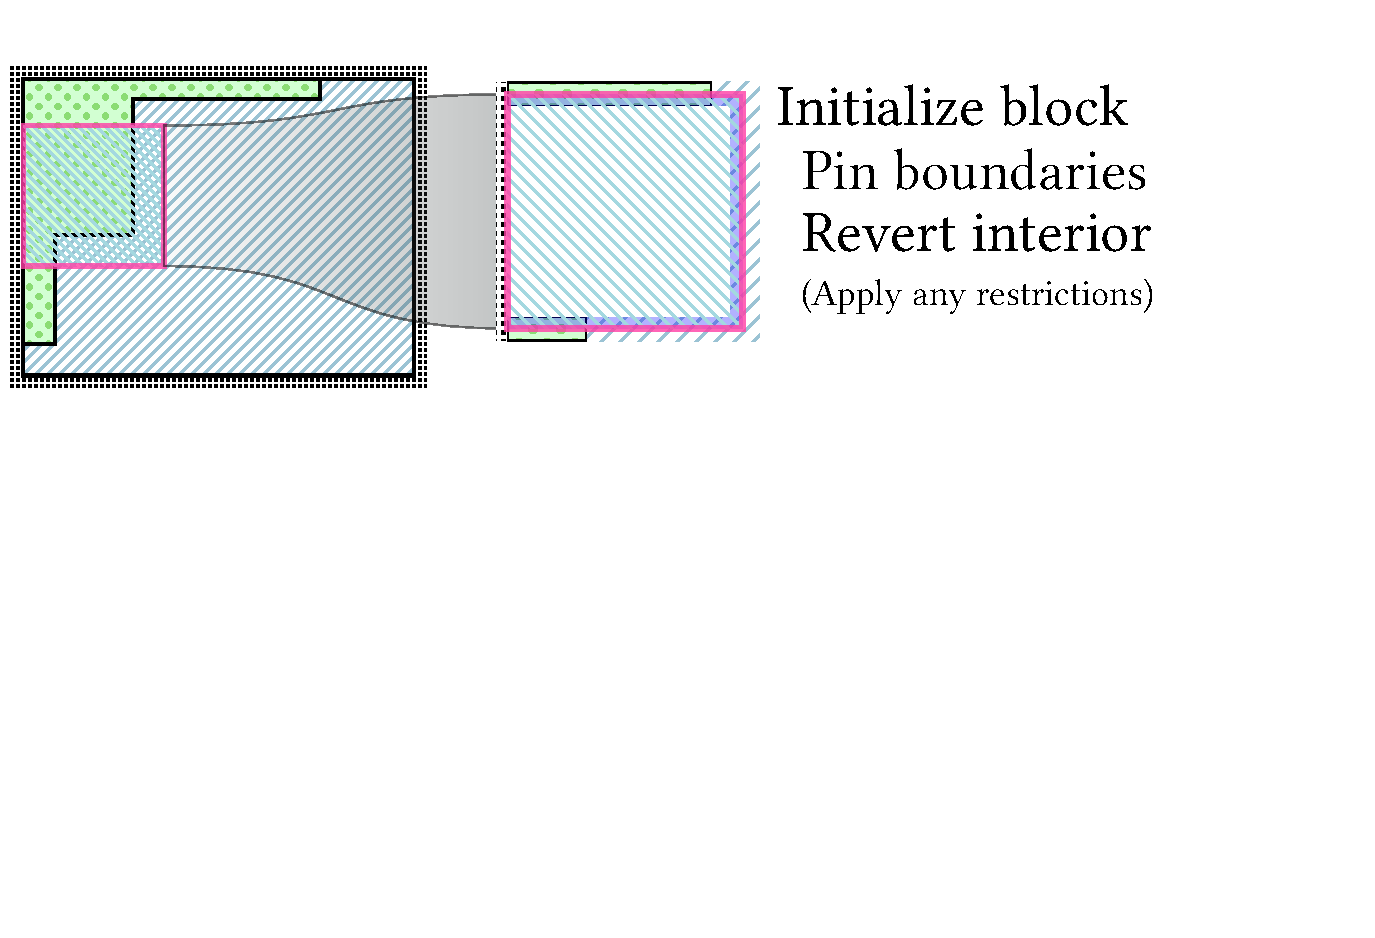
\includegraphics[width=\textwidth]{figs/poms_alg2.pdf}
    \end{figure}
  \end{frame}

  \begin{frame}[fragile]{Algorithm}
    \begin{figure}
      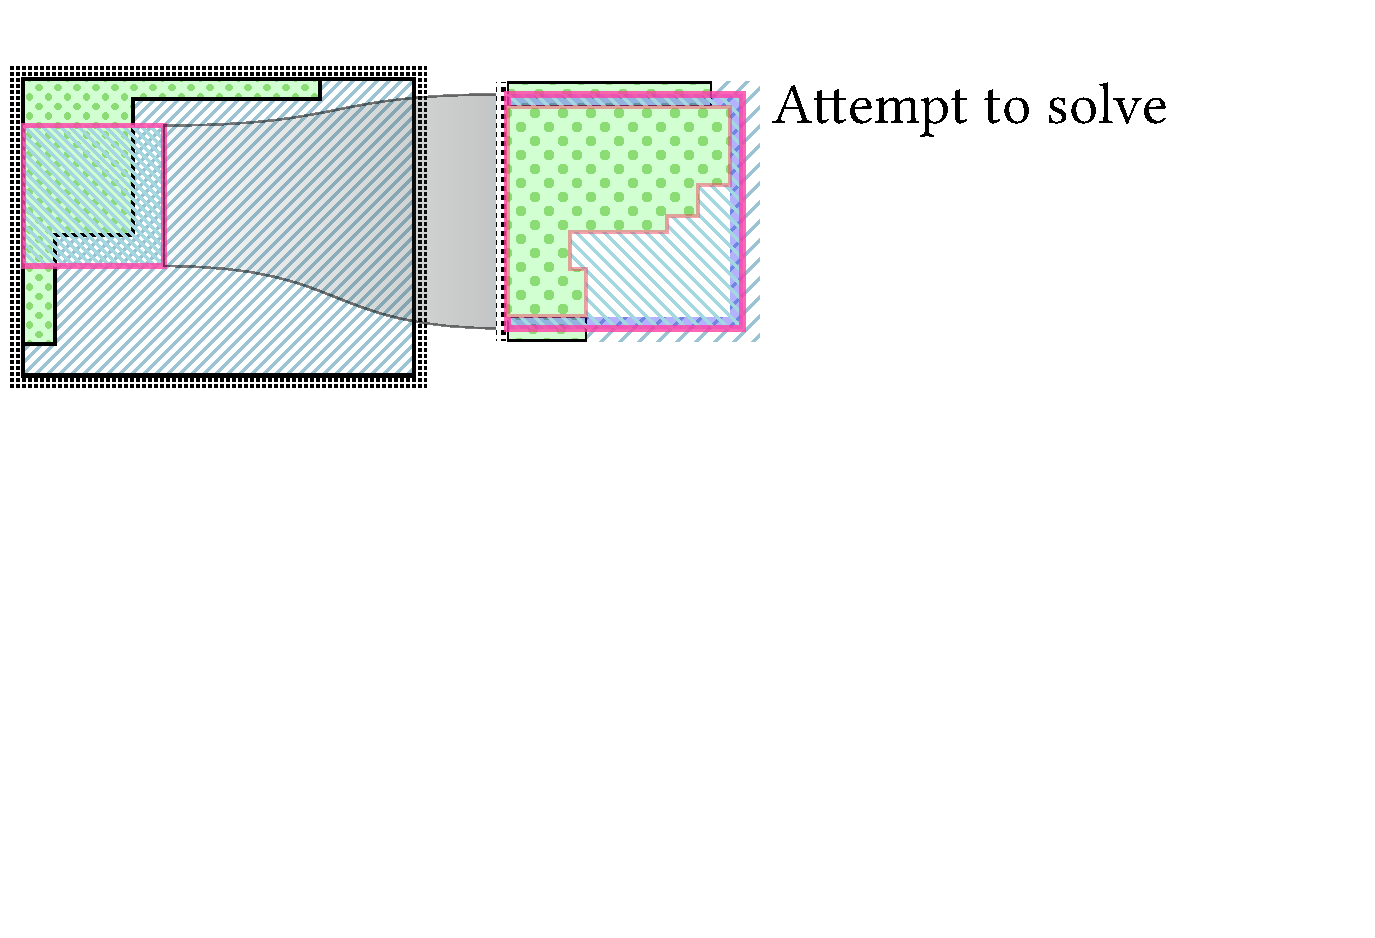
\includegraphics[width=\textwidth]{figs/poms_alg3.pdf}
    \end{figure}
  \end{frame}

  \begin{frame}[fragile]{Algorithm}
    \begin{figure}
      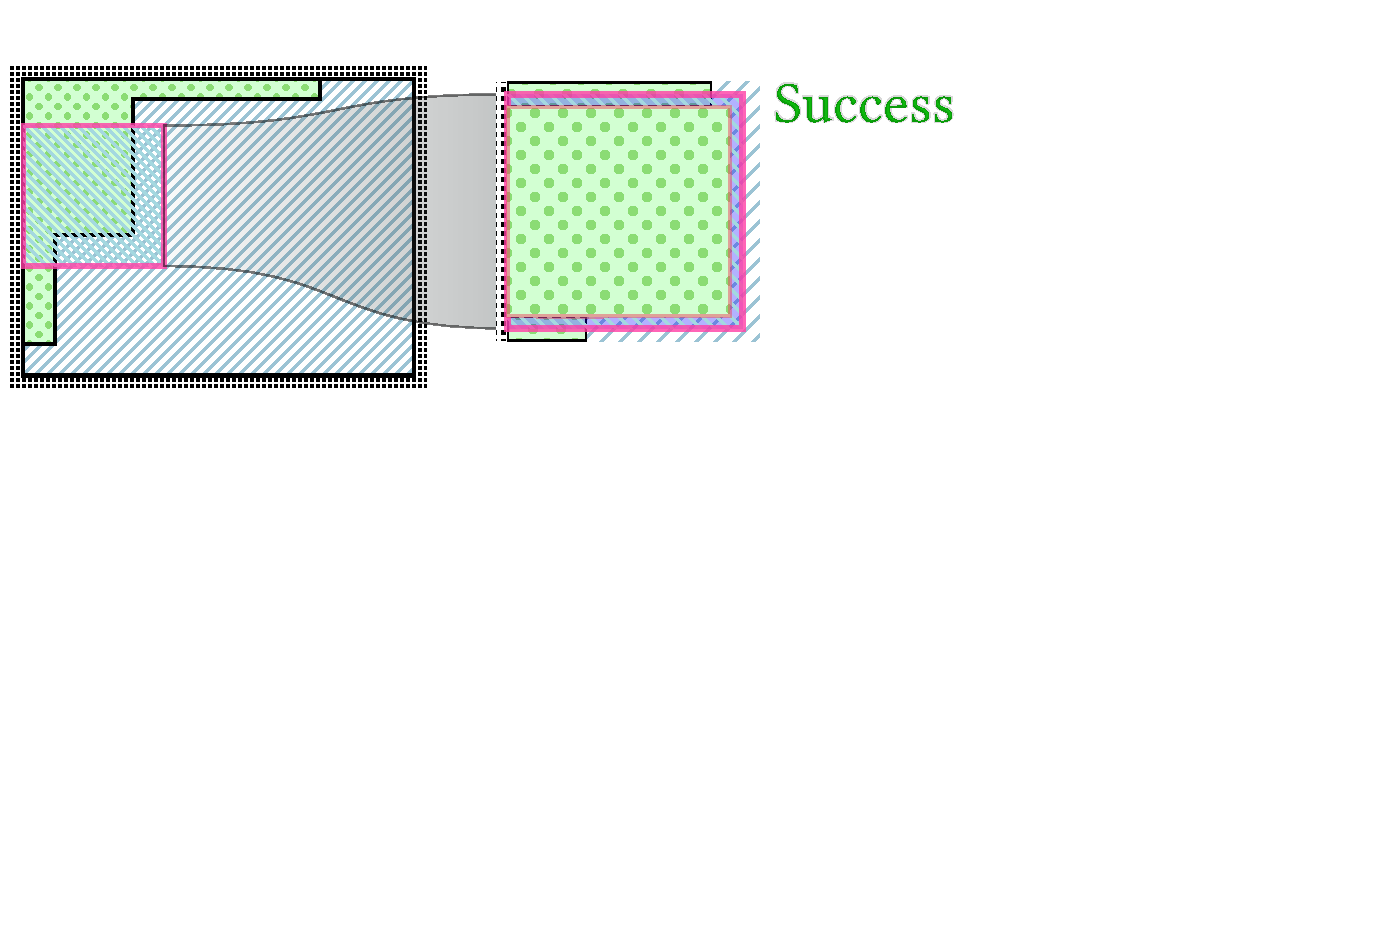
\includegraphics[width=\textwidth]{figs/poms_alg4.pdf}
    \end{figure}
  \end{frame}

  \begin{frame}[fragile]{Algorithm}
    \begin{figure}
      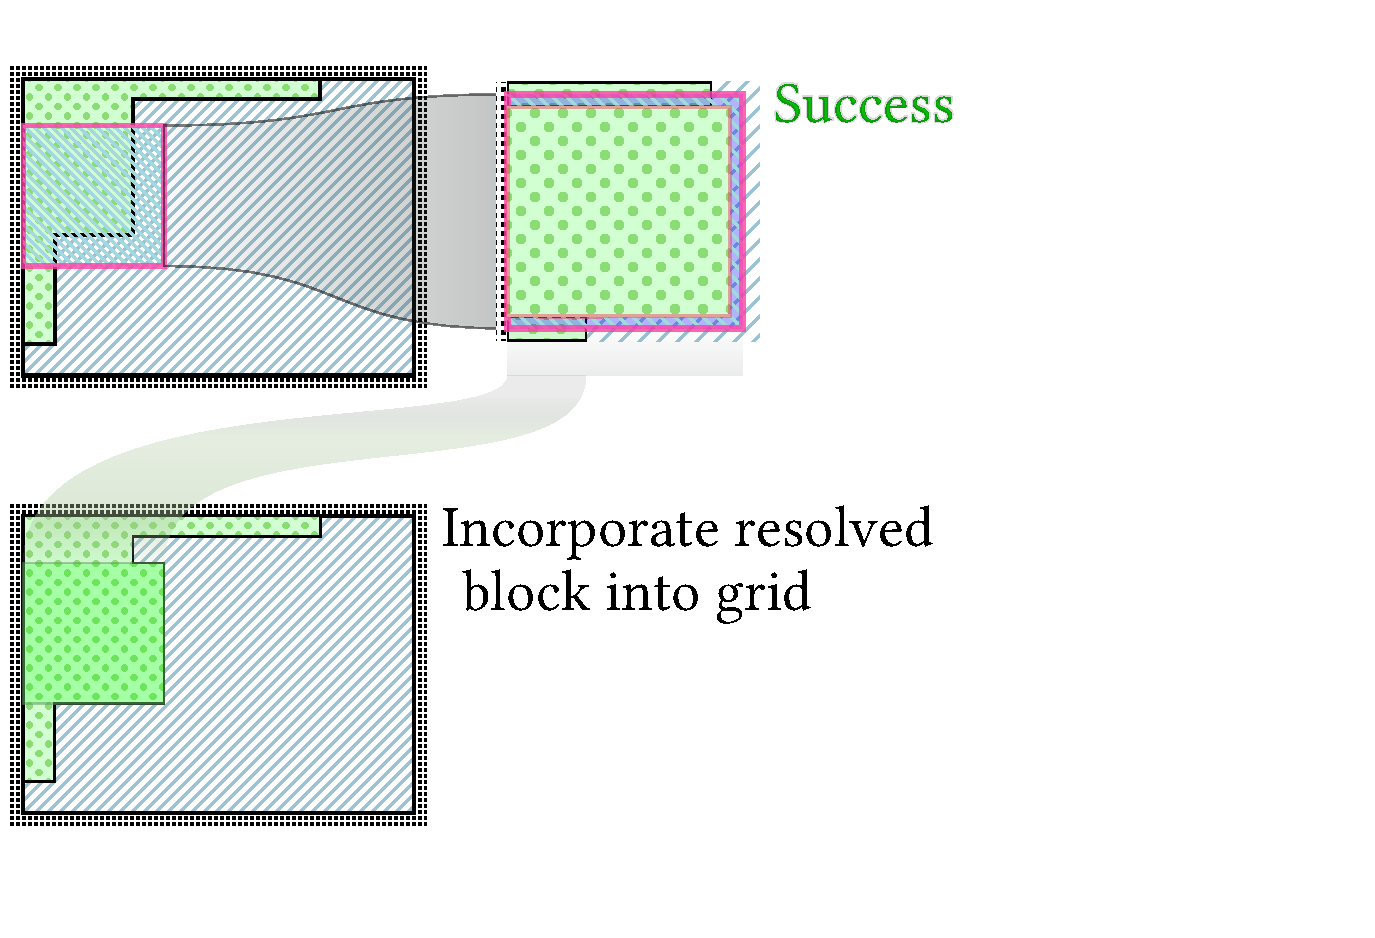
\includegraphics[width=\textwidth]{figs/poms_alg4_5.pdf}
    \end{figure}
  \end{frame}

  \begin{frame}[fragile]{Algorithm}
    \begin{figure}
      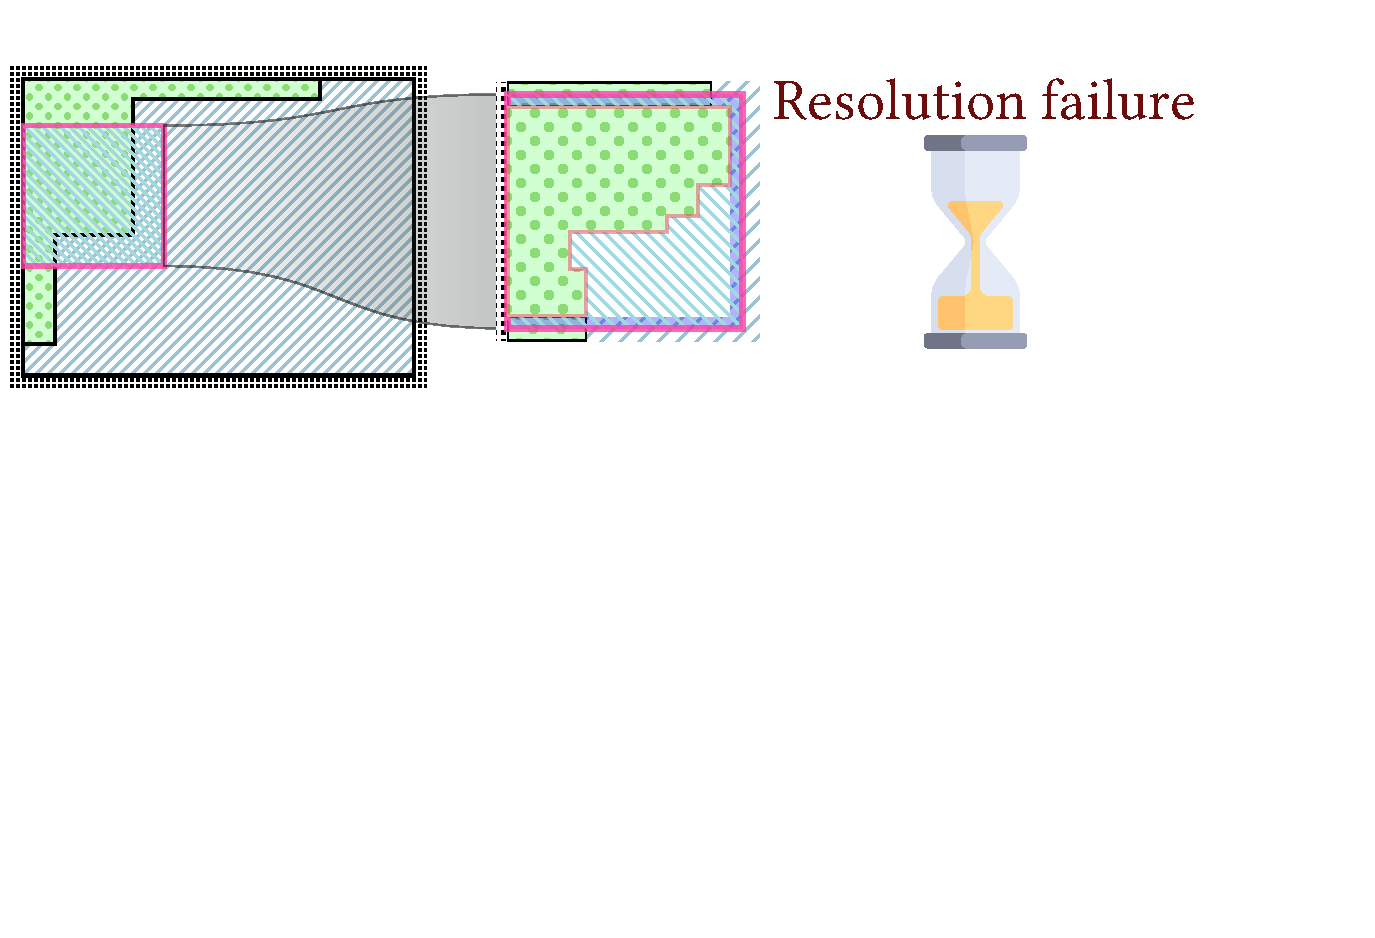
\includegraphics[width=\textwidth]{figs/poms_alg5.pdf}
    \end{figure}
  \end{frame}

  \begin{frame}[fragile]{Algorithm}
    \begin{figure}
      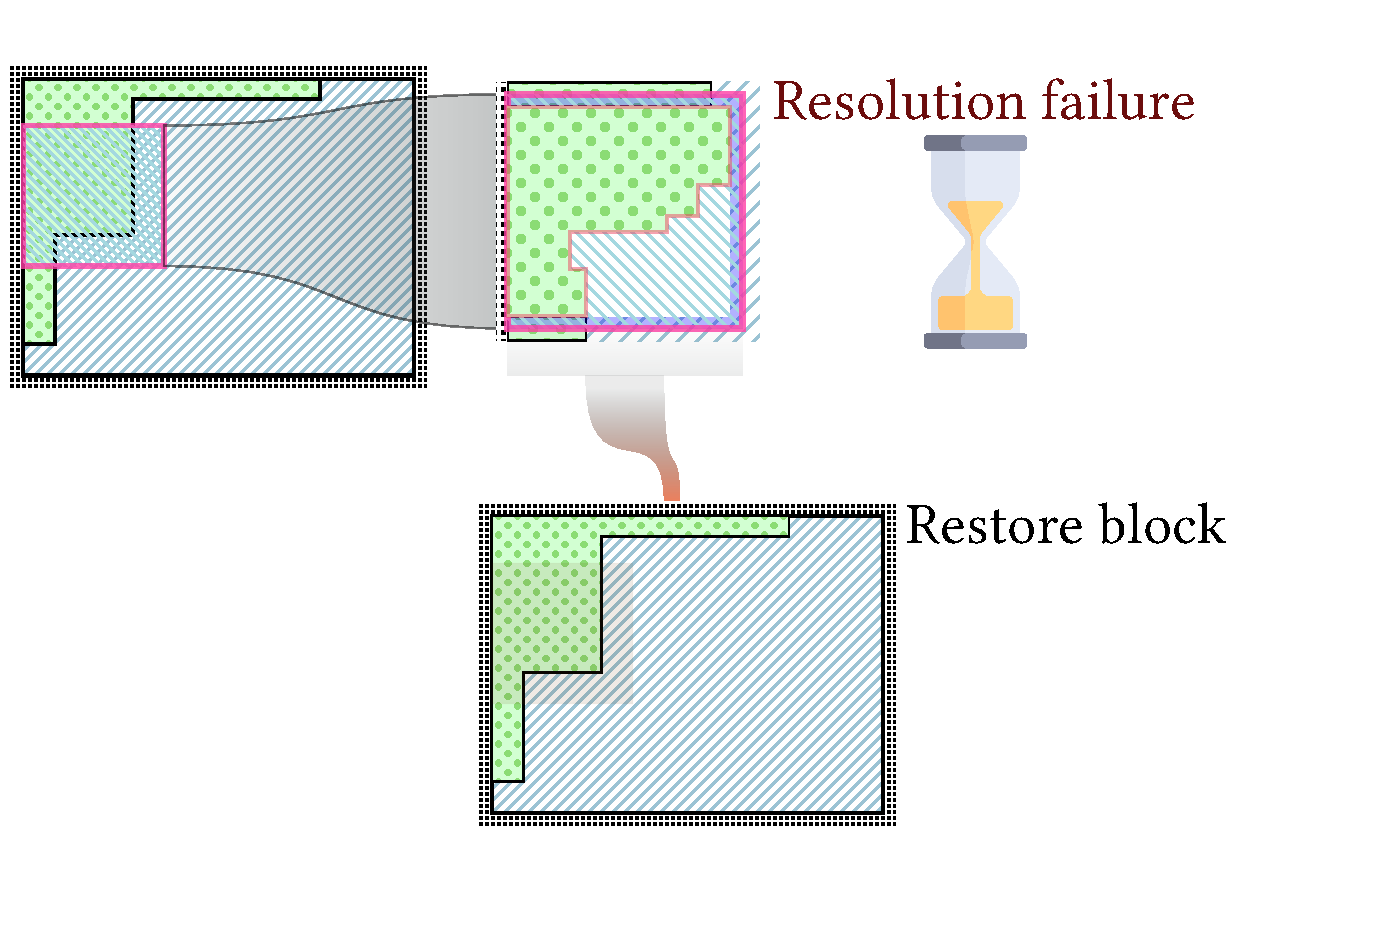
\includegraphics[width=\textwidth]{figs/poms_alg5_1.pdf}
    \end{figure}
  \end{frame}

  \begin{frame}[fragile]{Algorithm}
    \begin{figure}
      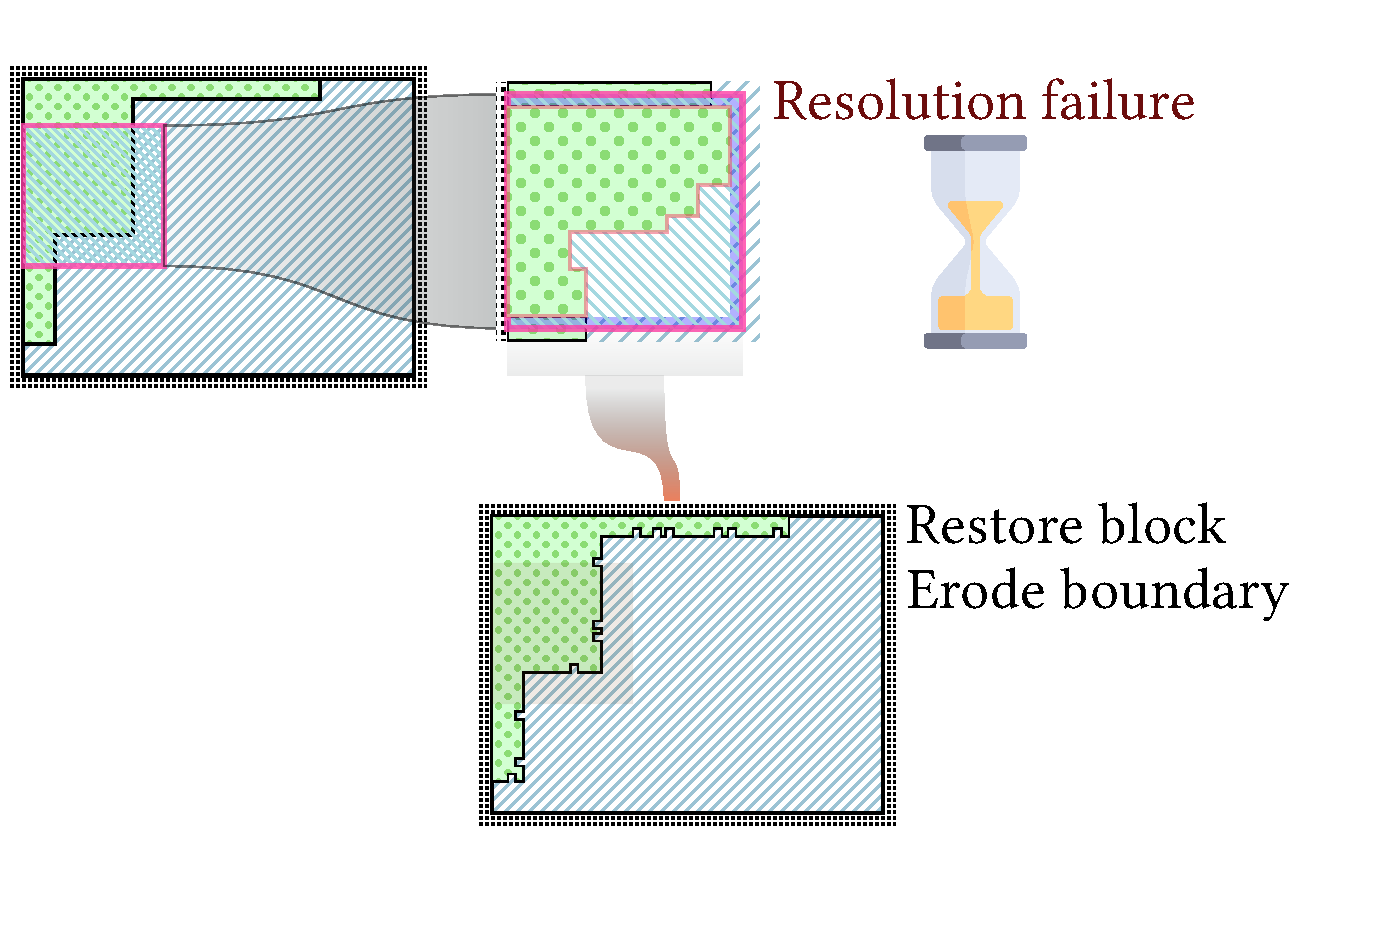
\includegraphics[width=\textwidth]{figs/poms_alg5_2.pdf}
    \end{figure}
  \end{frame}

  \begin{frame}[fragile]{Algorithm}
    \begin{figure}
      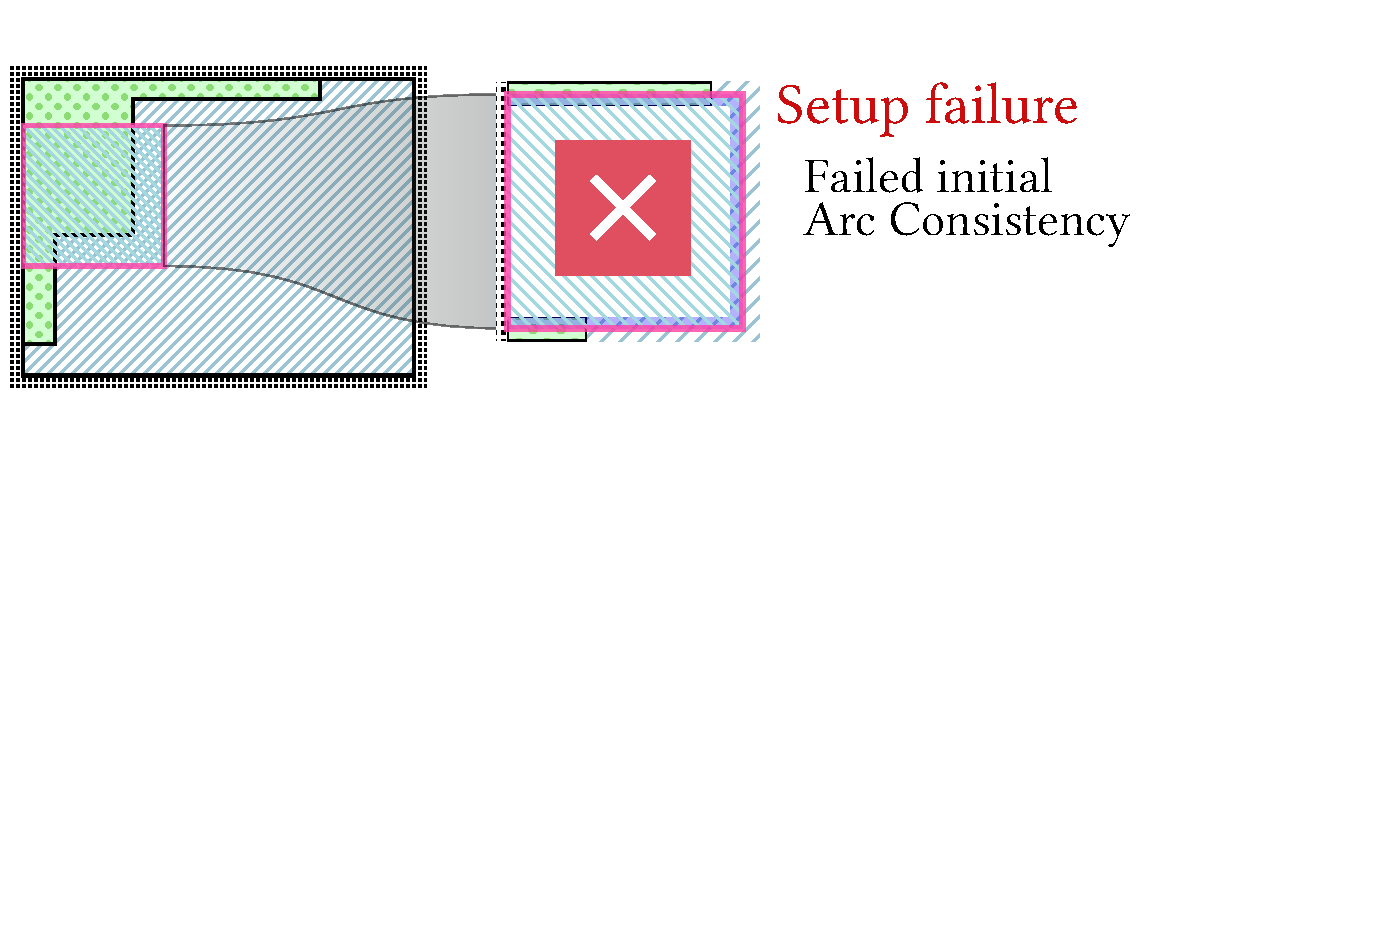
\includegraphics[width=\textwidth]{figs/poms_alg6_1.pdf}
    \end{figure}
  \end{frame}

  \begin{frame}[fragile]{Algorithm}
    \begin{figure}
      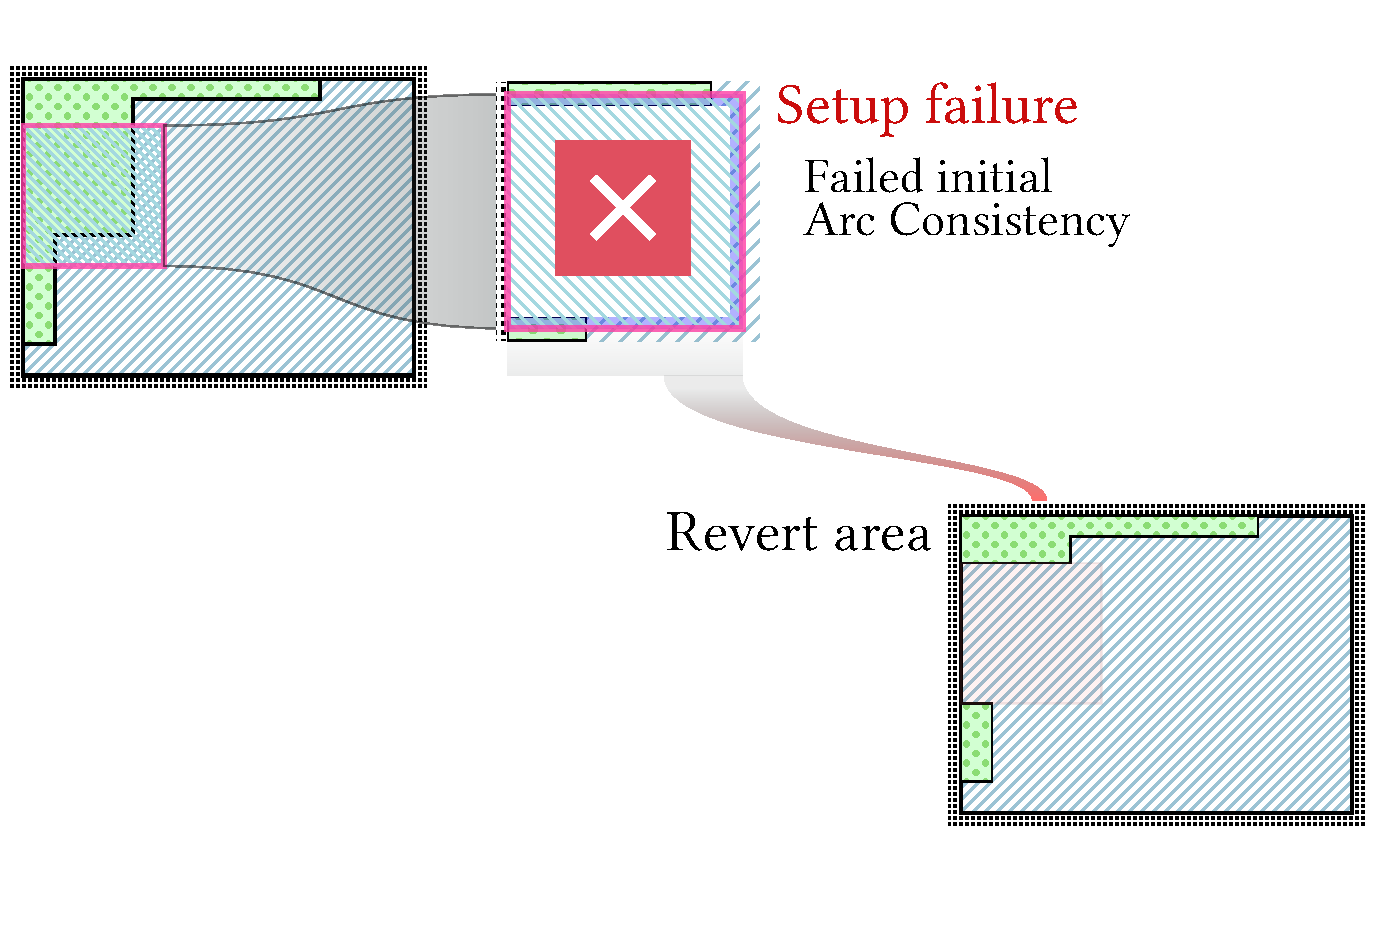
\includegraphics[width=\textwidth]{figs/poms_alg6_2.pdf}
    \end{figure}
  \end{frame}

  \begin{frame}[fragile]{Algorithm}
    \begin{figure}
      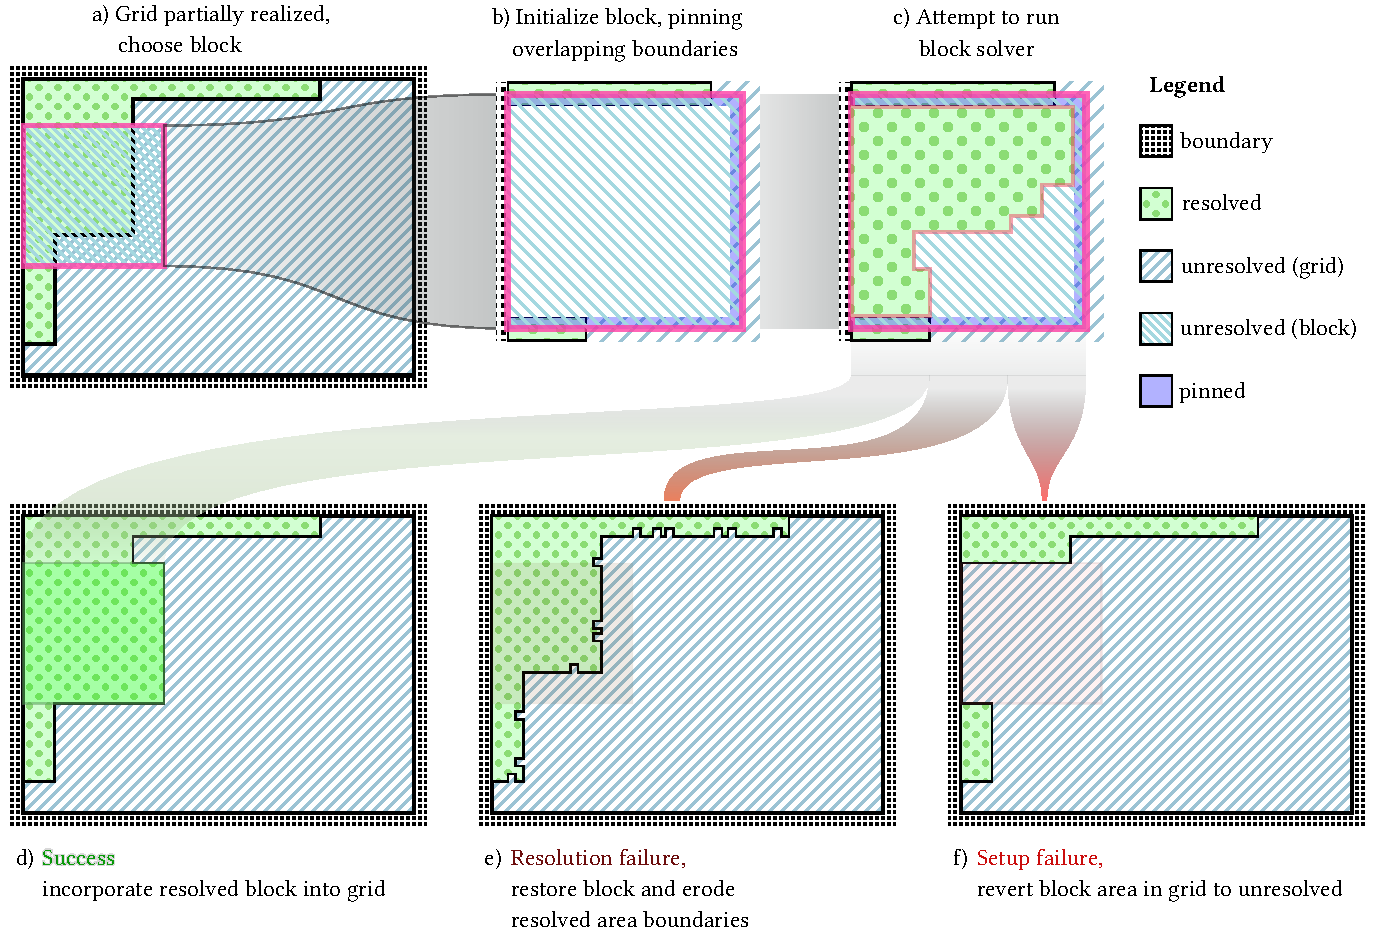
\includegraphics[width=\textwidth]{figs/poms_figalg.pdf}
    \end{figure}
  \end{frame}

%  \begin{frame}[fragile]{Algorithm}
%    \begin{figure}
%      \textit{Pill Mortal} Tile Set
%
%      \movie[width=6cm,height=6cm,poster,autostart,repeat]{}{vid/pm_w.mp4}
%    \end{figure}
%  \end{frame}

%  \begin{frame}[fragile]{Algorithm}
%    \begin{figure}
%      LUNARSIGNALS' \textit{Overhead Action RPG Overworld} Tile Set
%
%      \movie[width=6cm,height=6cm,poster,autostart,repeat]{}{vid/oarpgo_x10_w.mp4}
%    \end{figure}
%  \end{frame}

  \begin{frame}[fragile]{Algorithm}

    \begin{figure}
      ThKaspar's \textit{Forest Micro} Tile Set

      \movie[width=6cm,height=6cm,poster,autostart,repeat]{}{vid/forestmicro_x5_w.mp4}
    \end{figure}
  \end{frame}

%  \begin{frame}[fragile]{Algorithm}
%    \begin{figure}
%      Choose Block
%      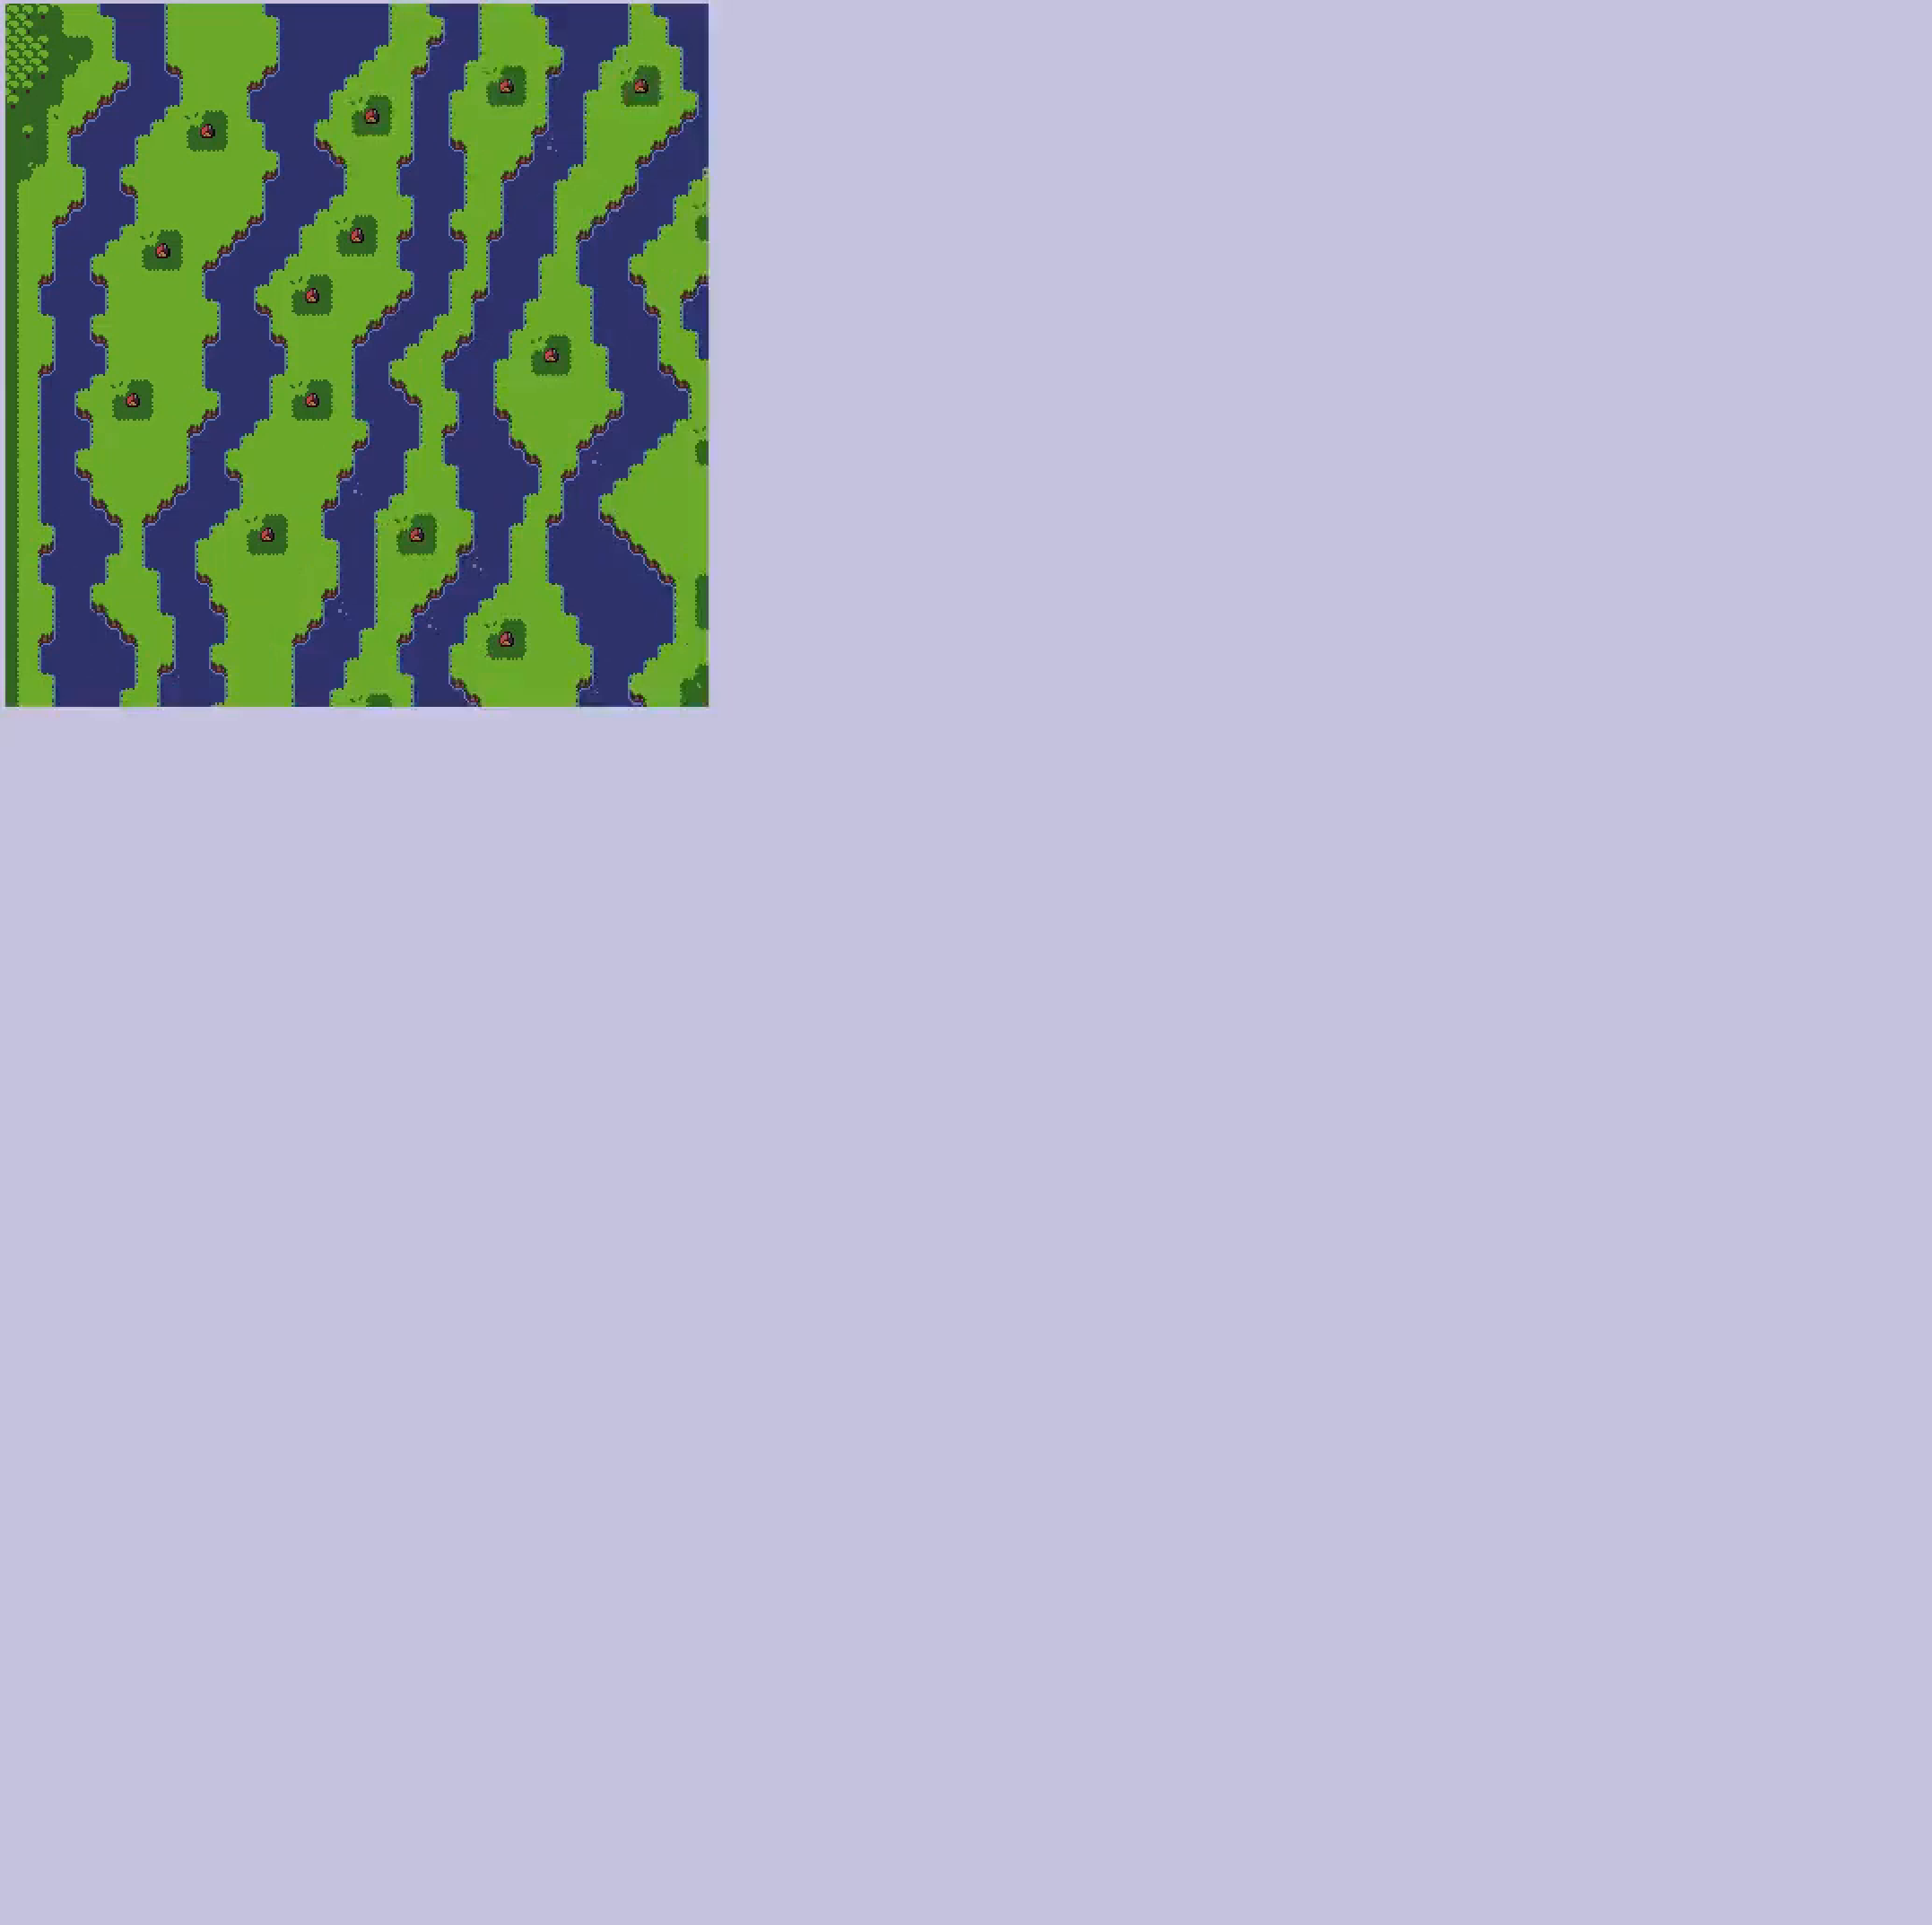
\includegraphics[width=6cm]{img/fm_0005.pdf}
%    \end{figure}
%  \end{frame}
%
%  \begin{frame}[fragile]{Algorithm}
%    \begin{figure}
%      Choose Block
%      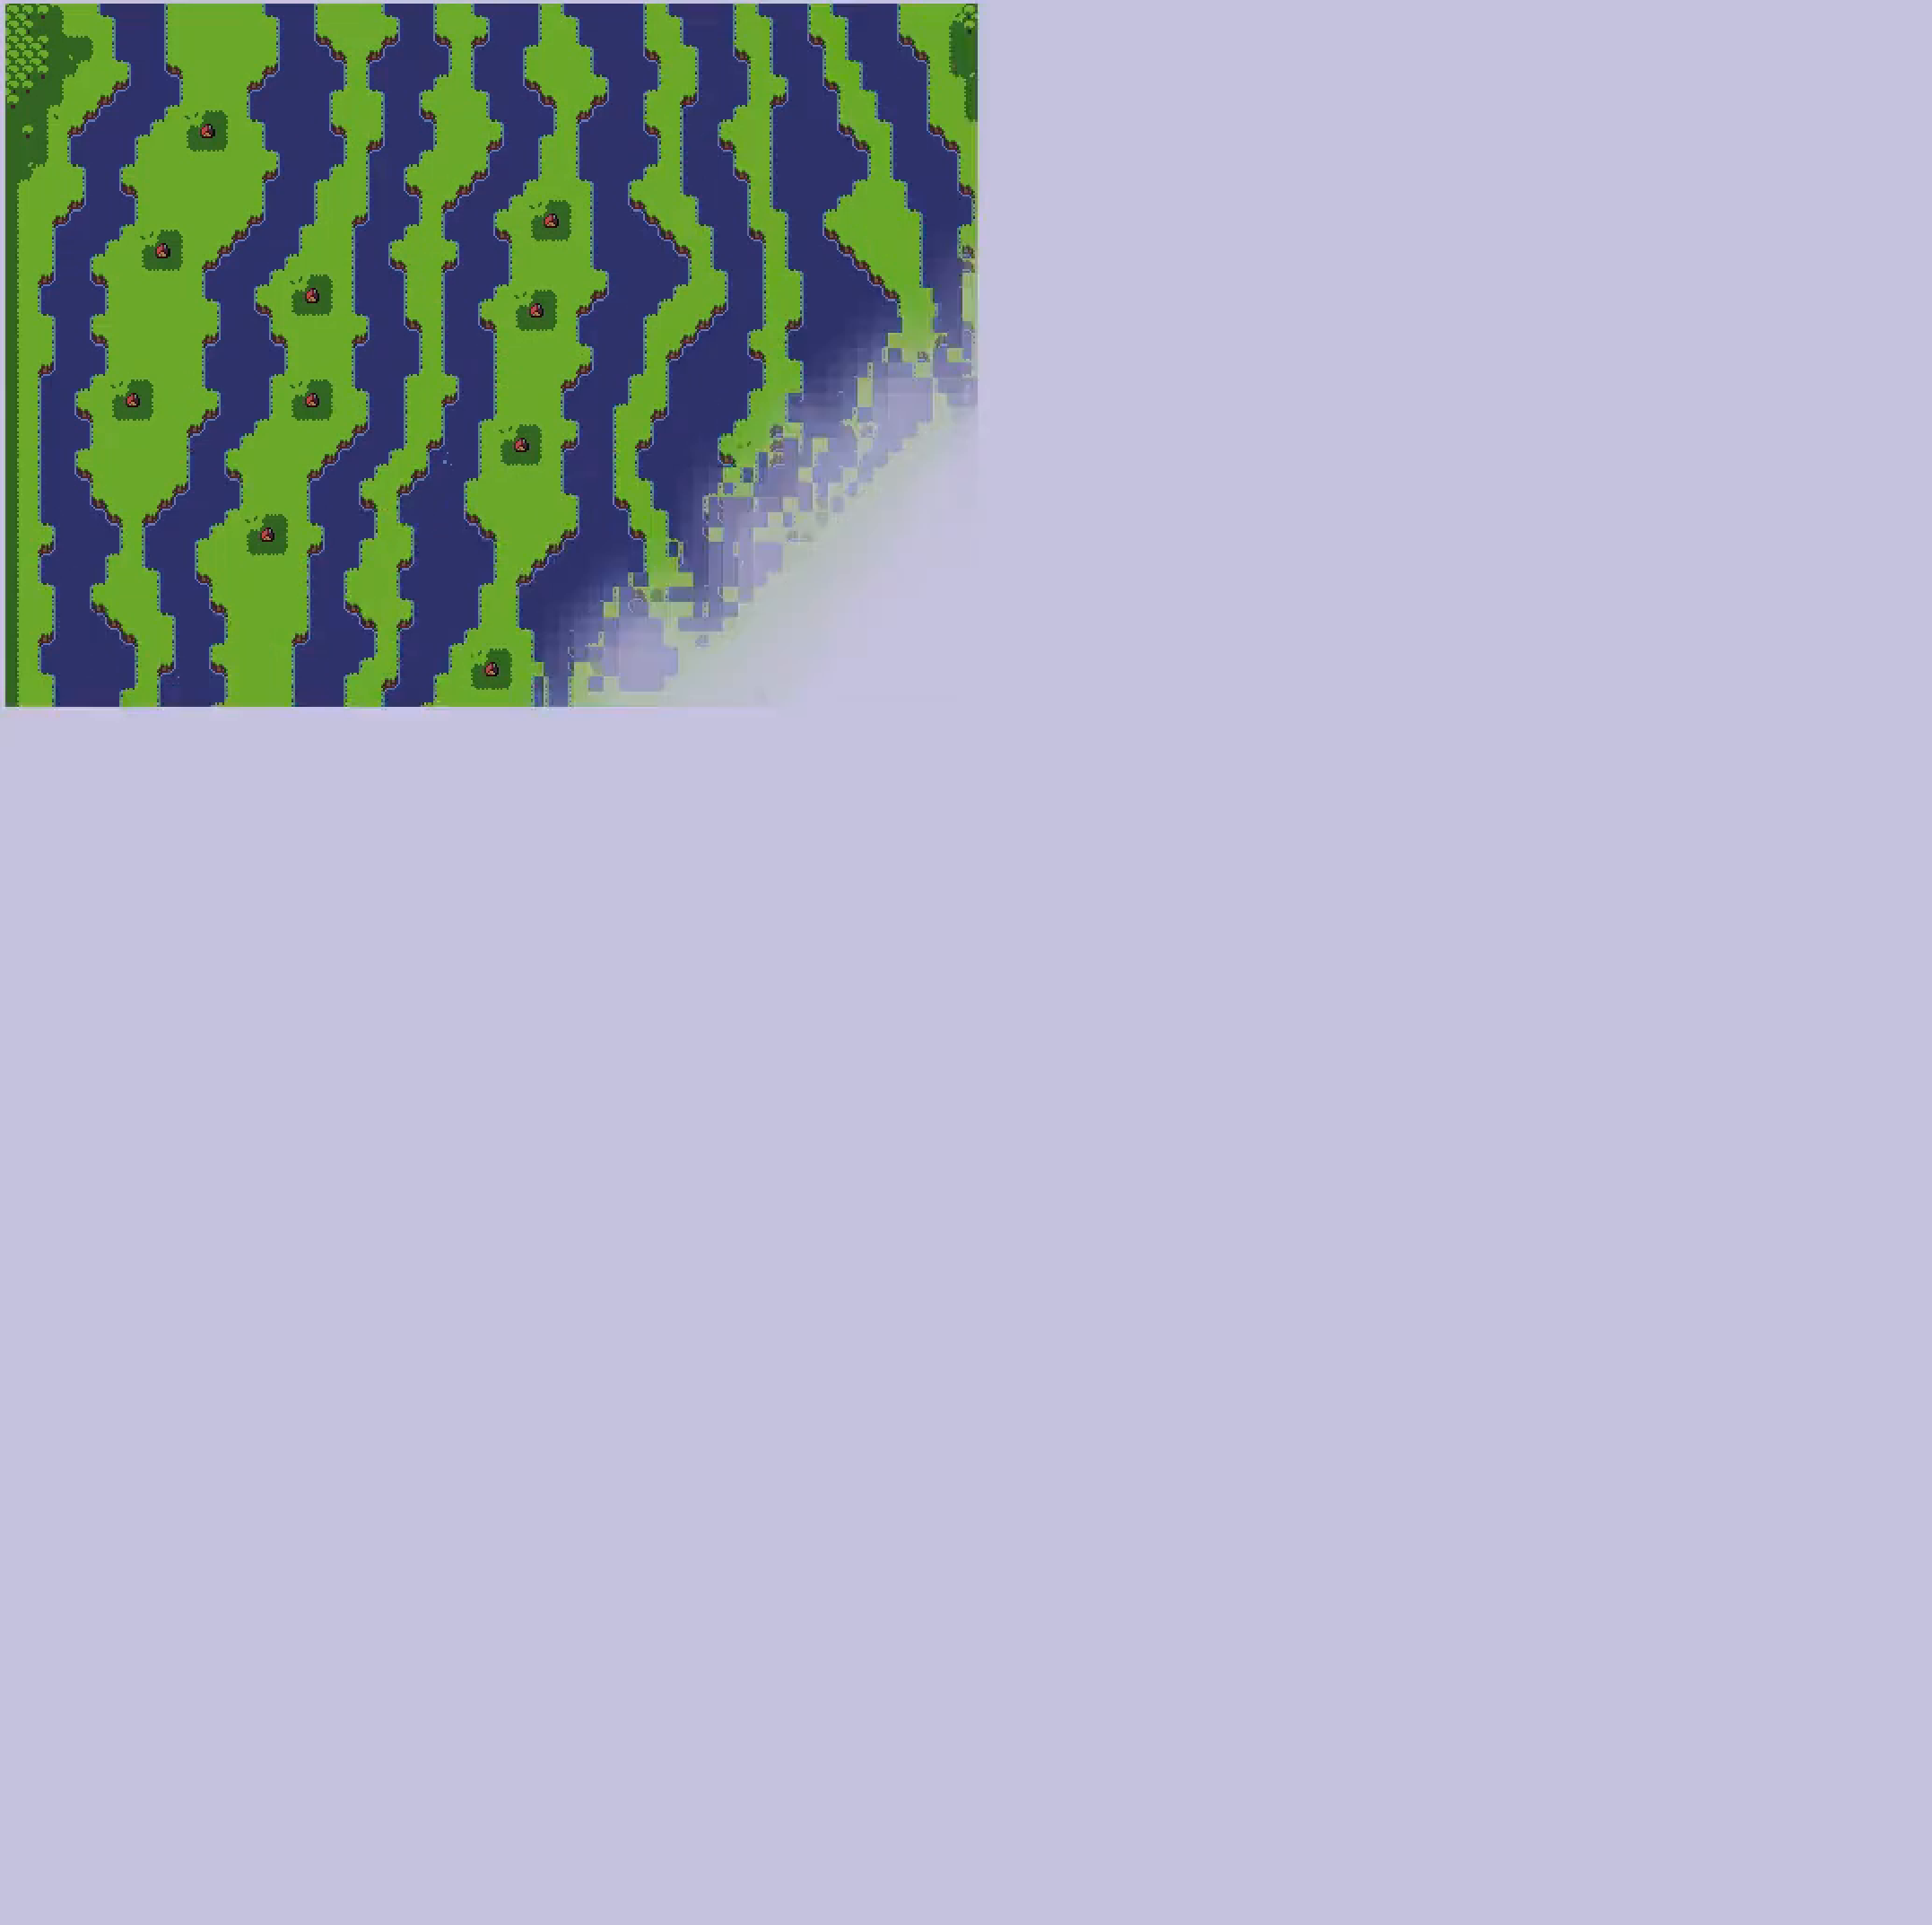
\includegraphics[width=6cm]{img/fm_0006.pdf}
%    \end{figure}
%  \end{frame}

  \begin{frame}[fragile]{Algorithm}
    \begin{figure}
      Revert Block

      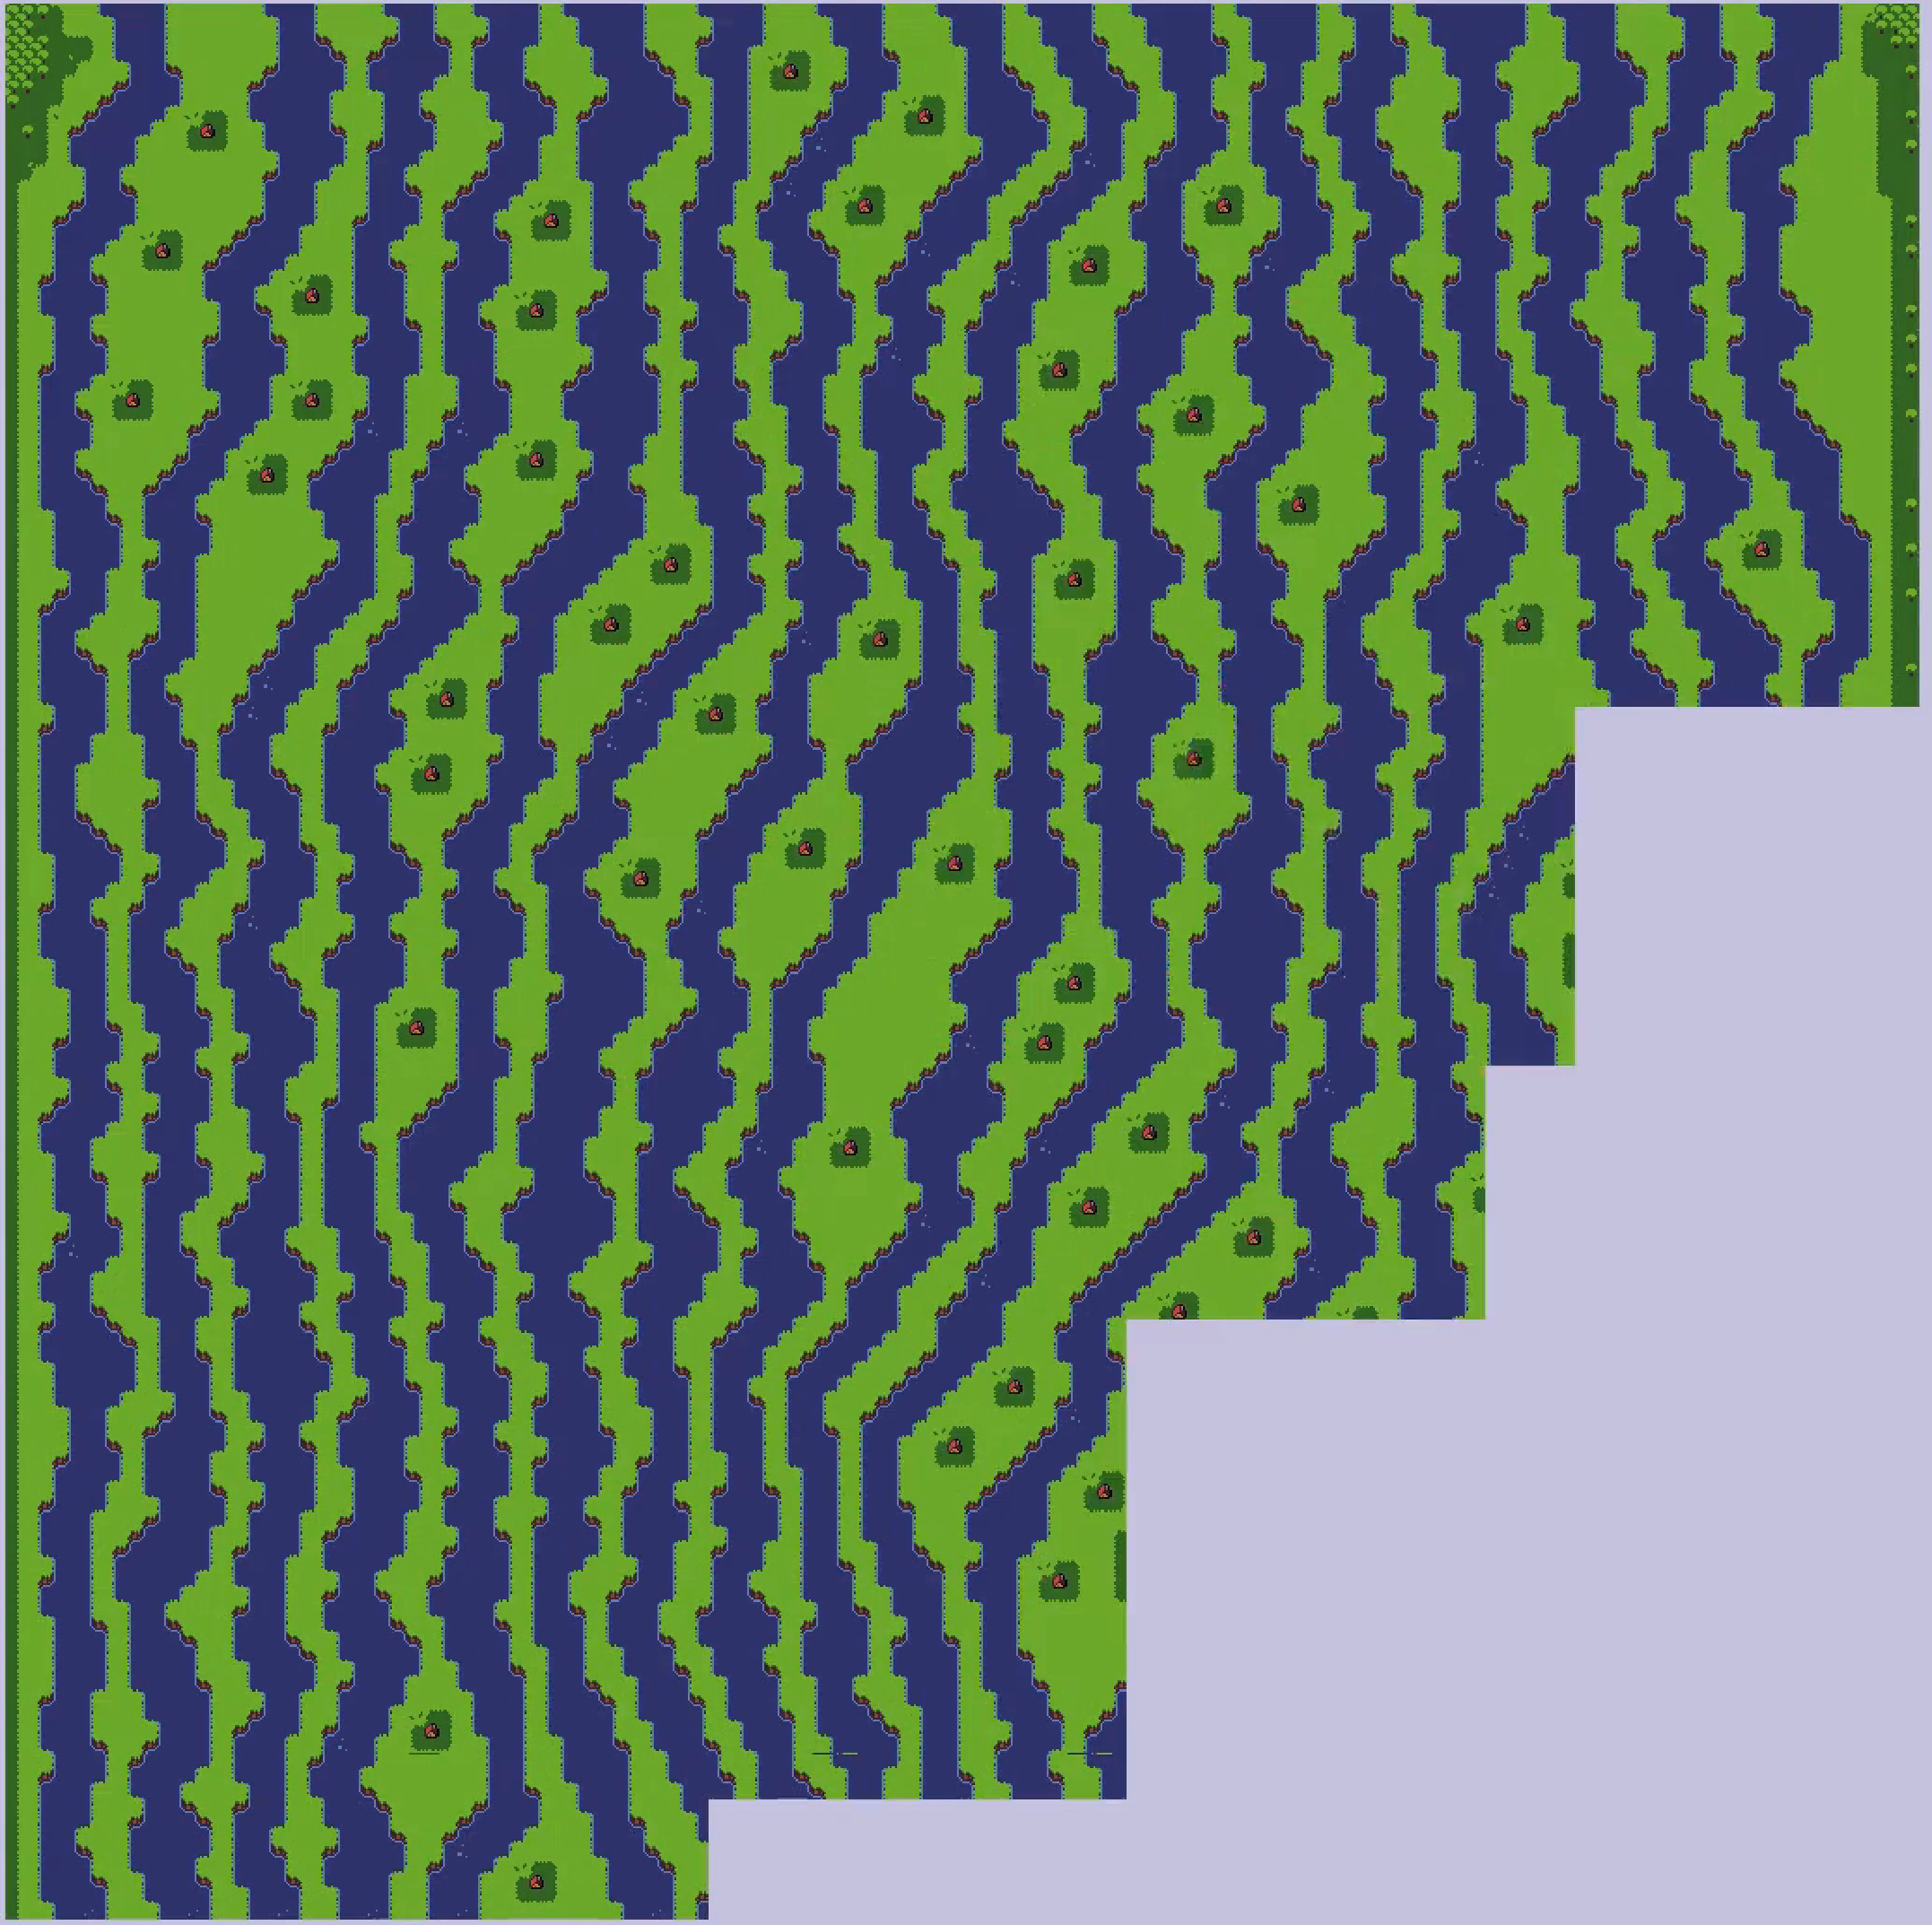
\includegraphics[width=6cm]{img/fm_0023.pdf}
    \end{figure}
  \end{frame}

  \begin{frame}[fragile]{Algorithm}
    \begin{figure}
      Revert Block

      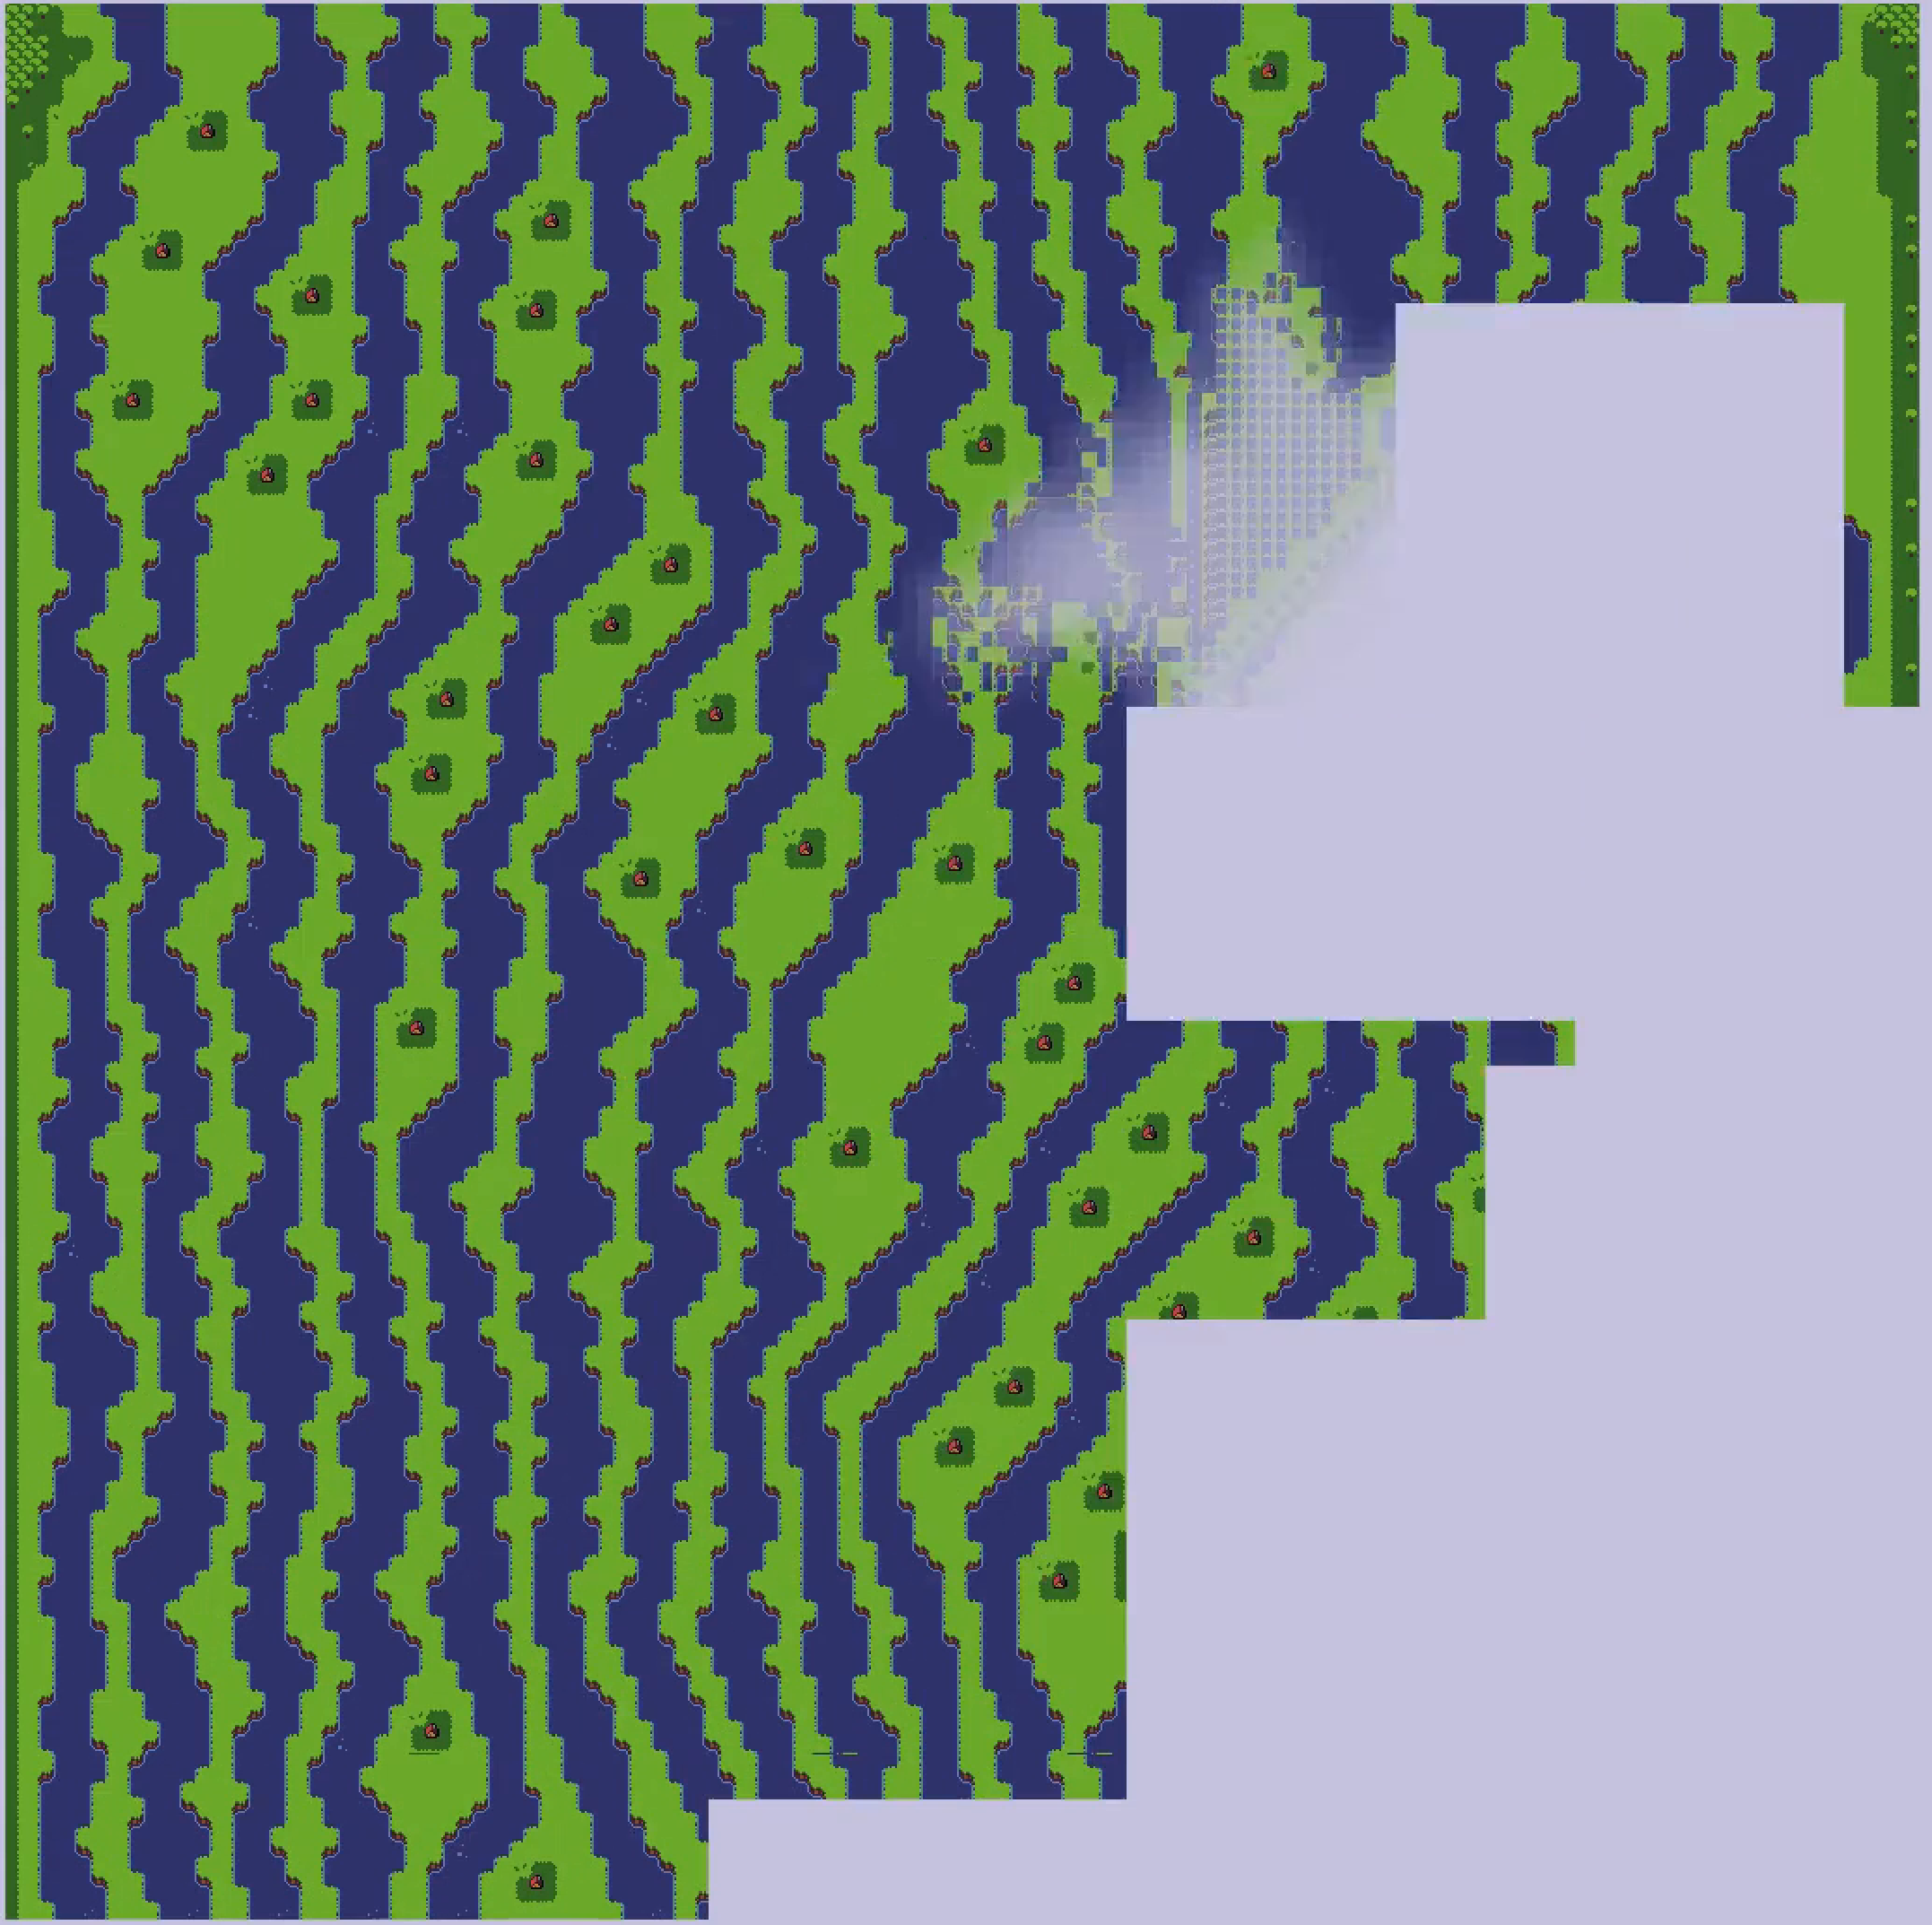
\includegraphics[width=6cm]{img/fm_0024.pdf}
    \end{figure}
  \end{frame}

  \begin{frame}[fragile]{Algorithm}

    \begin{figure}
      Erode Boundary

      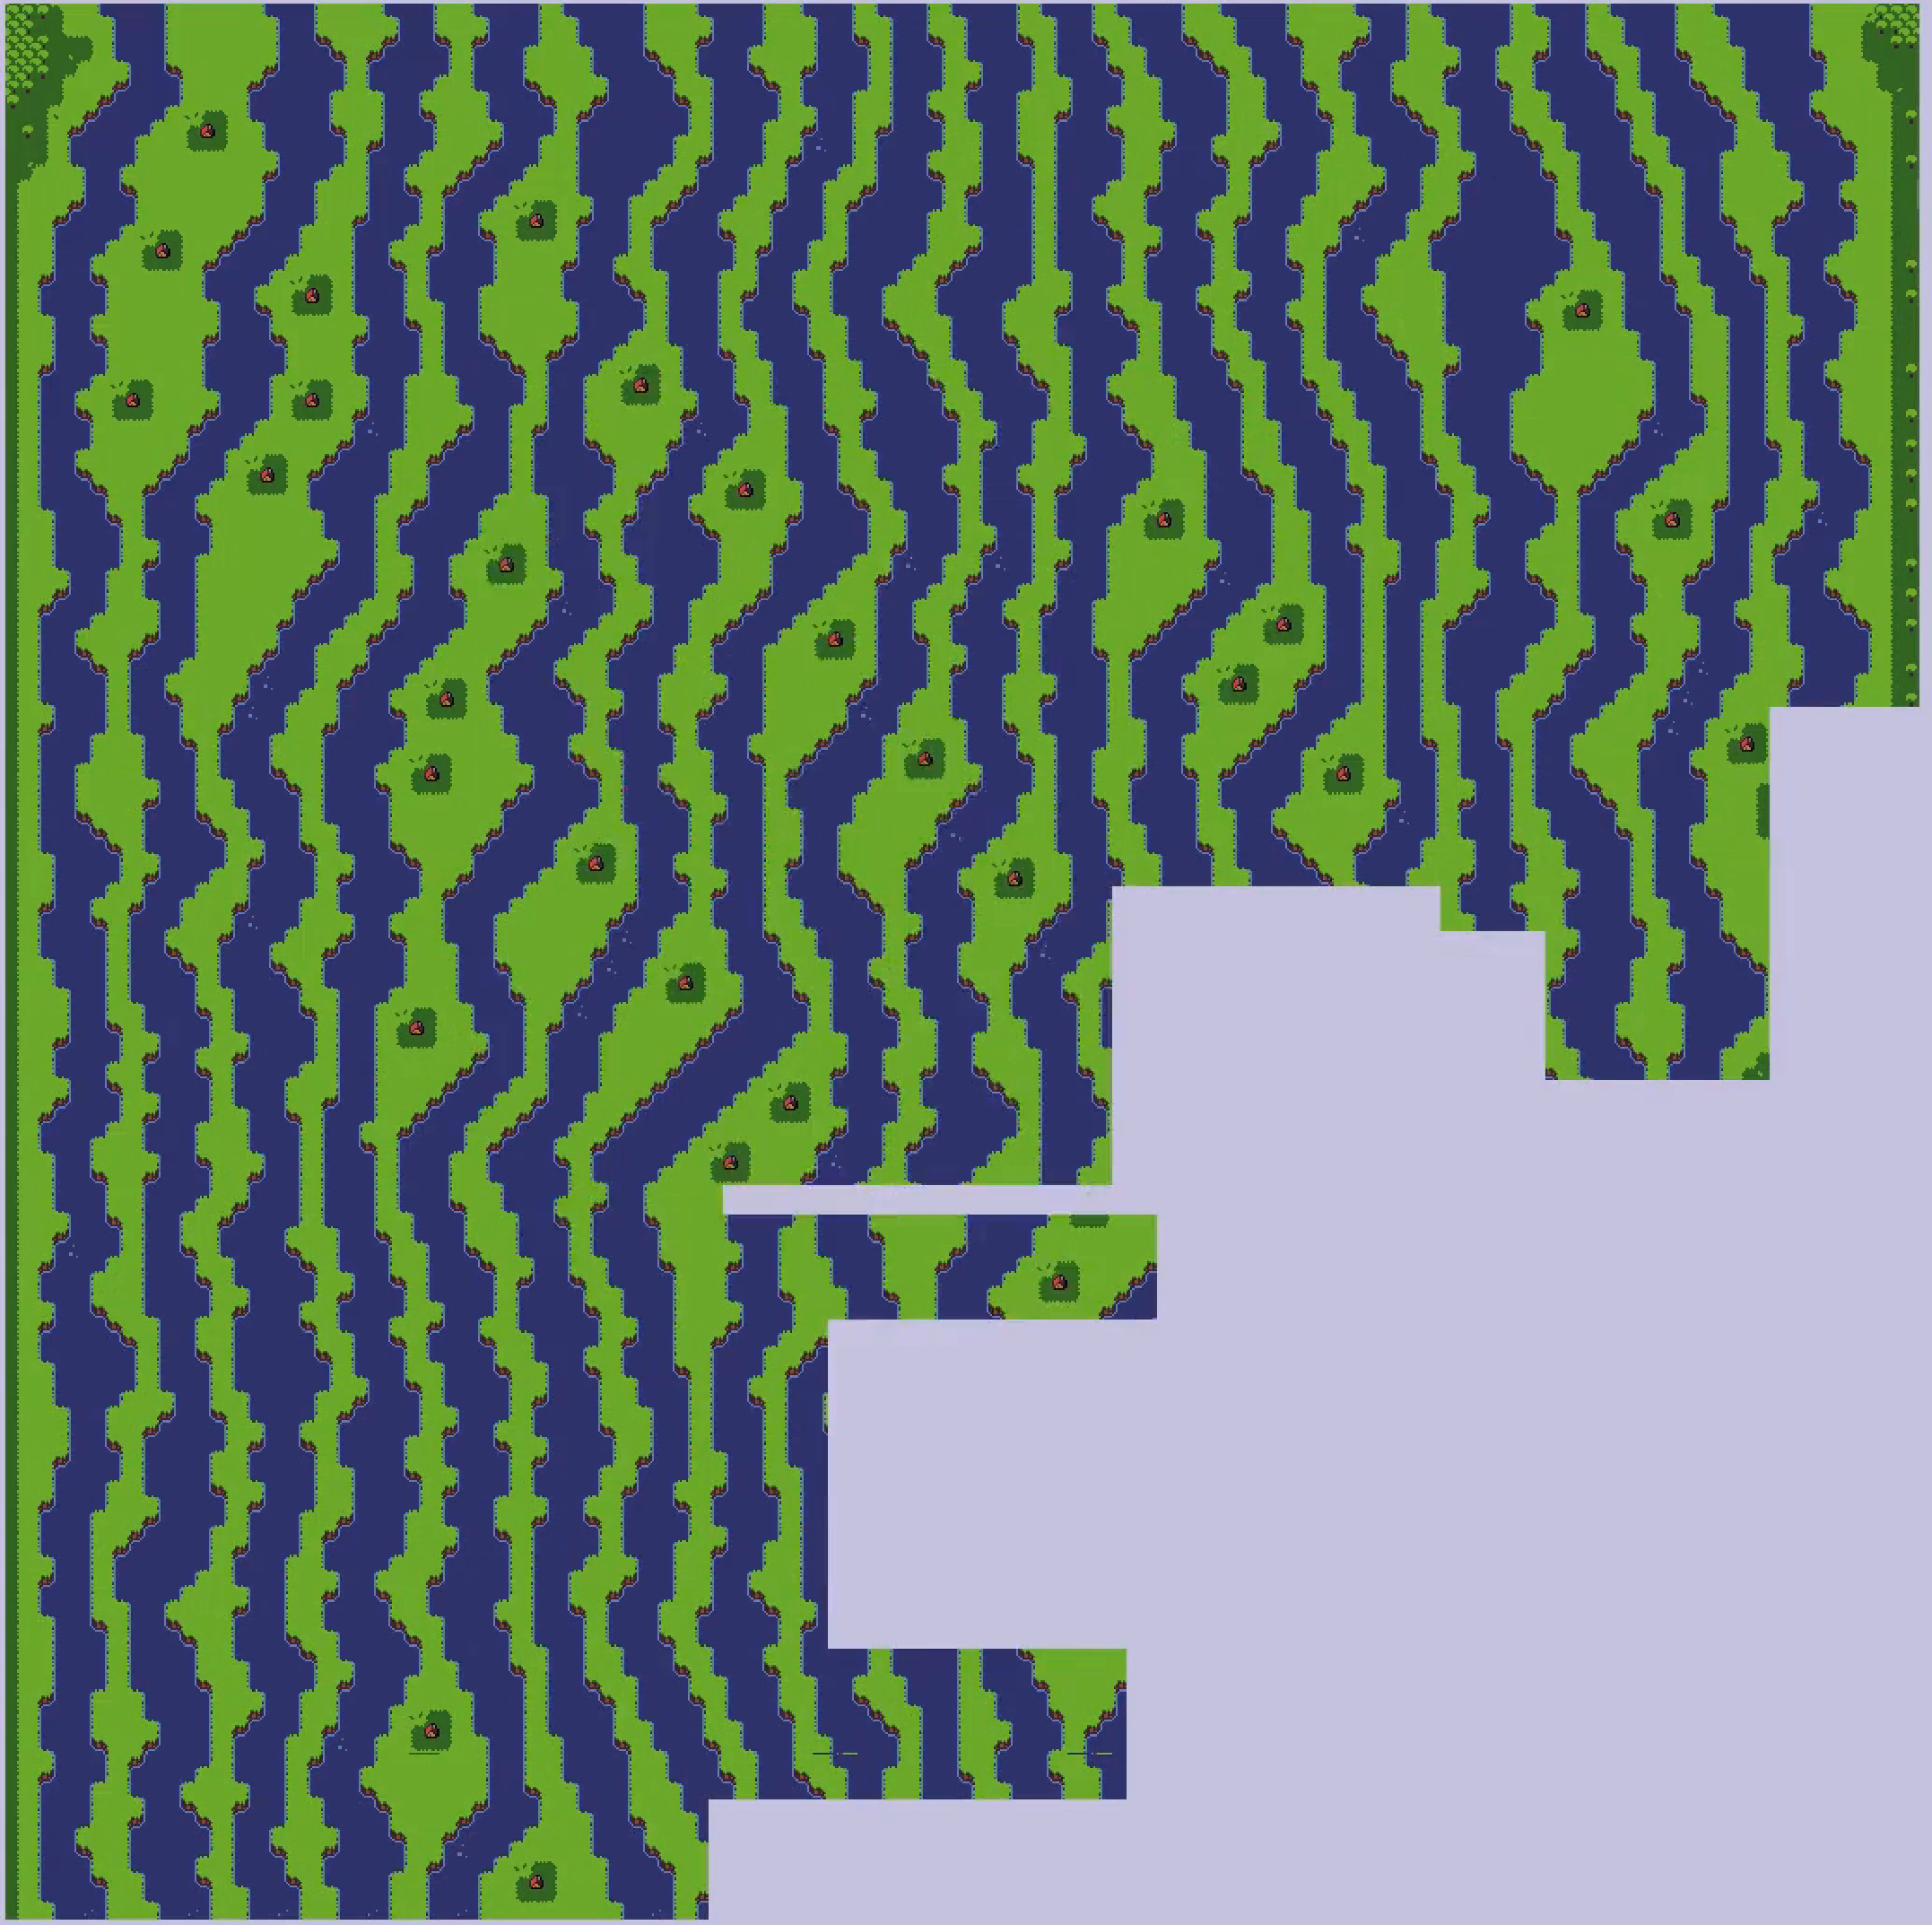
\includegraphics[width=6cm]{img/fm_0035.pdf}
    \end{figure}
  \end{frame}

  \begin{frame}[fragile]{Algorithm}

    \begin{figure}
      Erode Boundary

      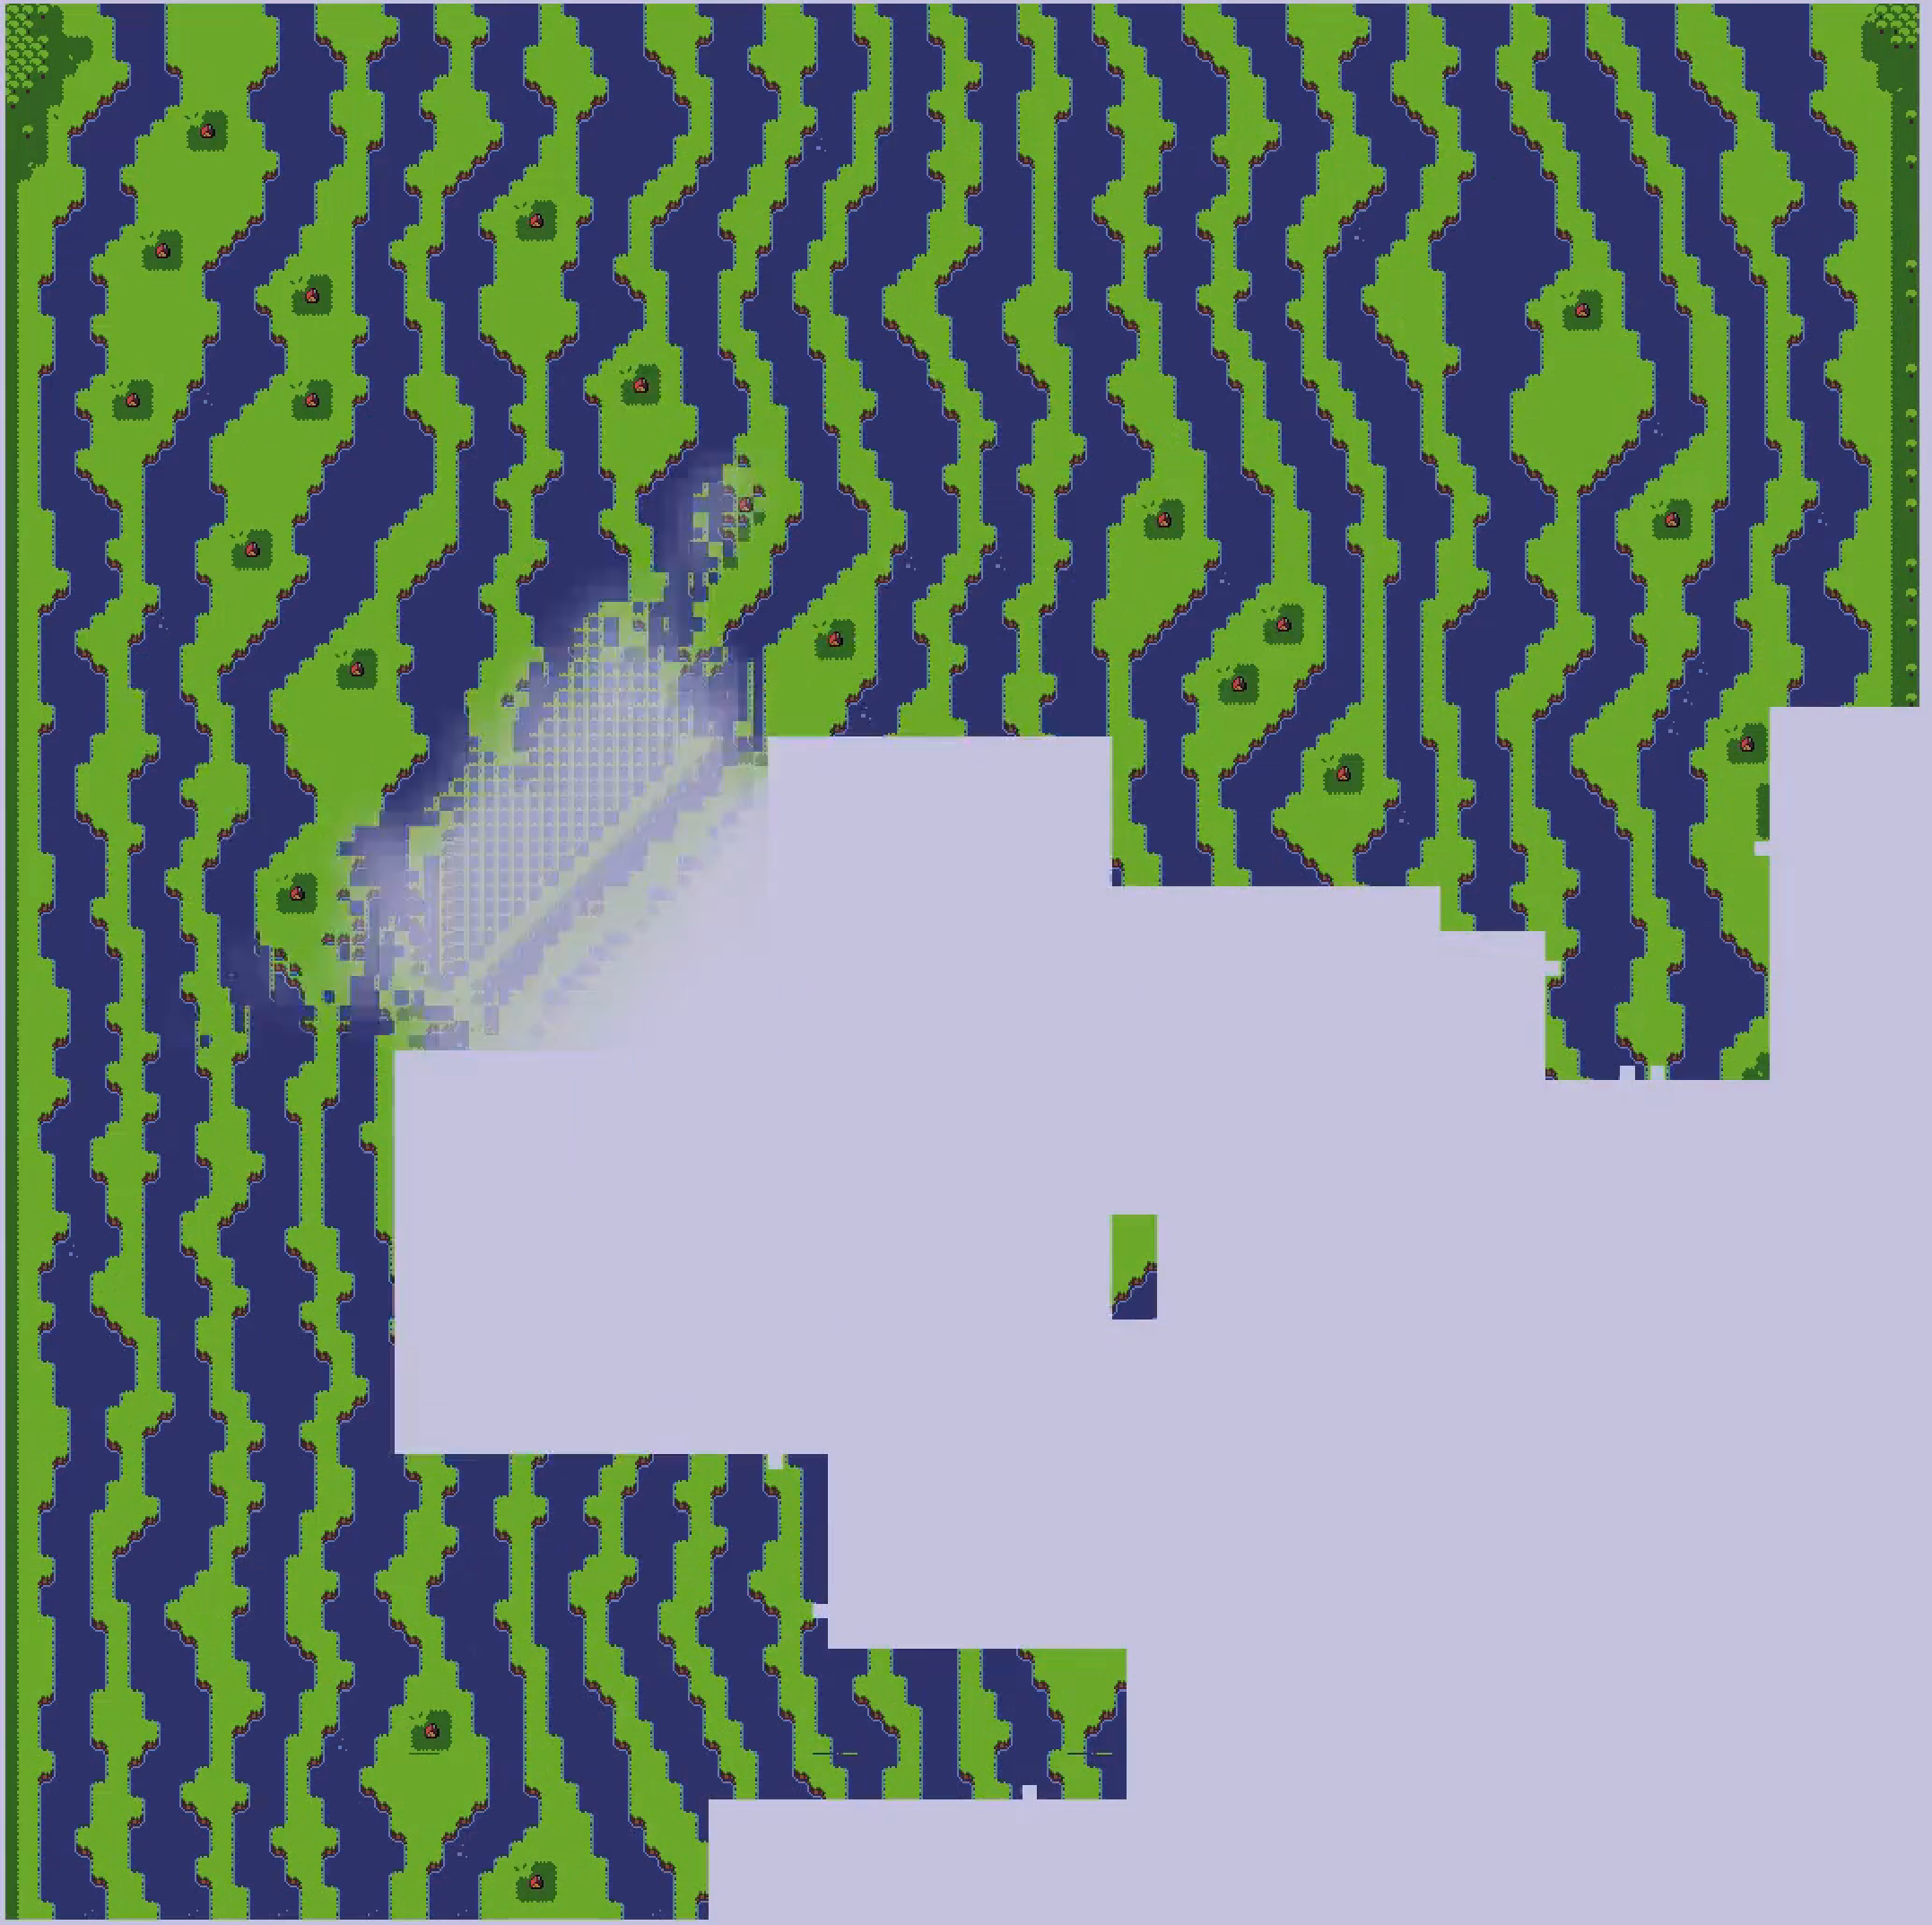
\includegraphics[width=6cm]{img/fm_0036.pdf}
    \end{figure}
  \end{frame}

%  \begin{frame}[fragile]{Algorithm}
%    Choose Block
%    \begin{figure}
%      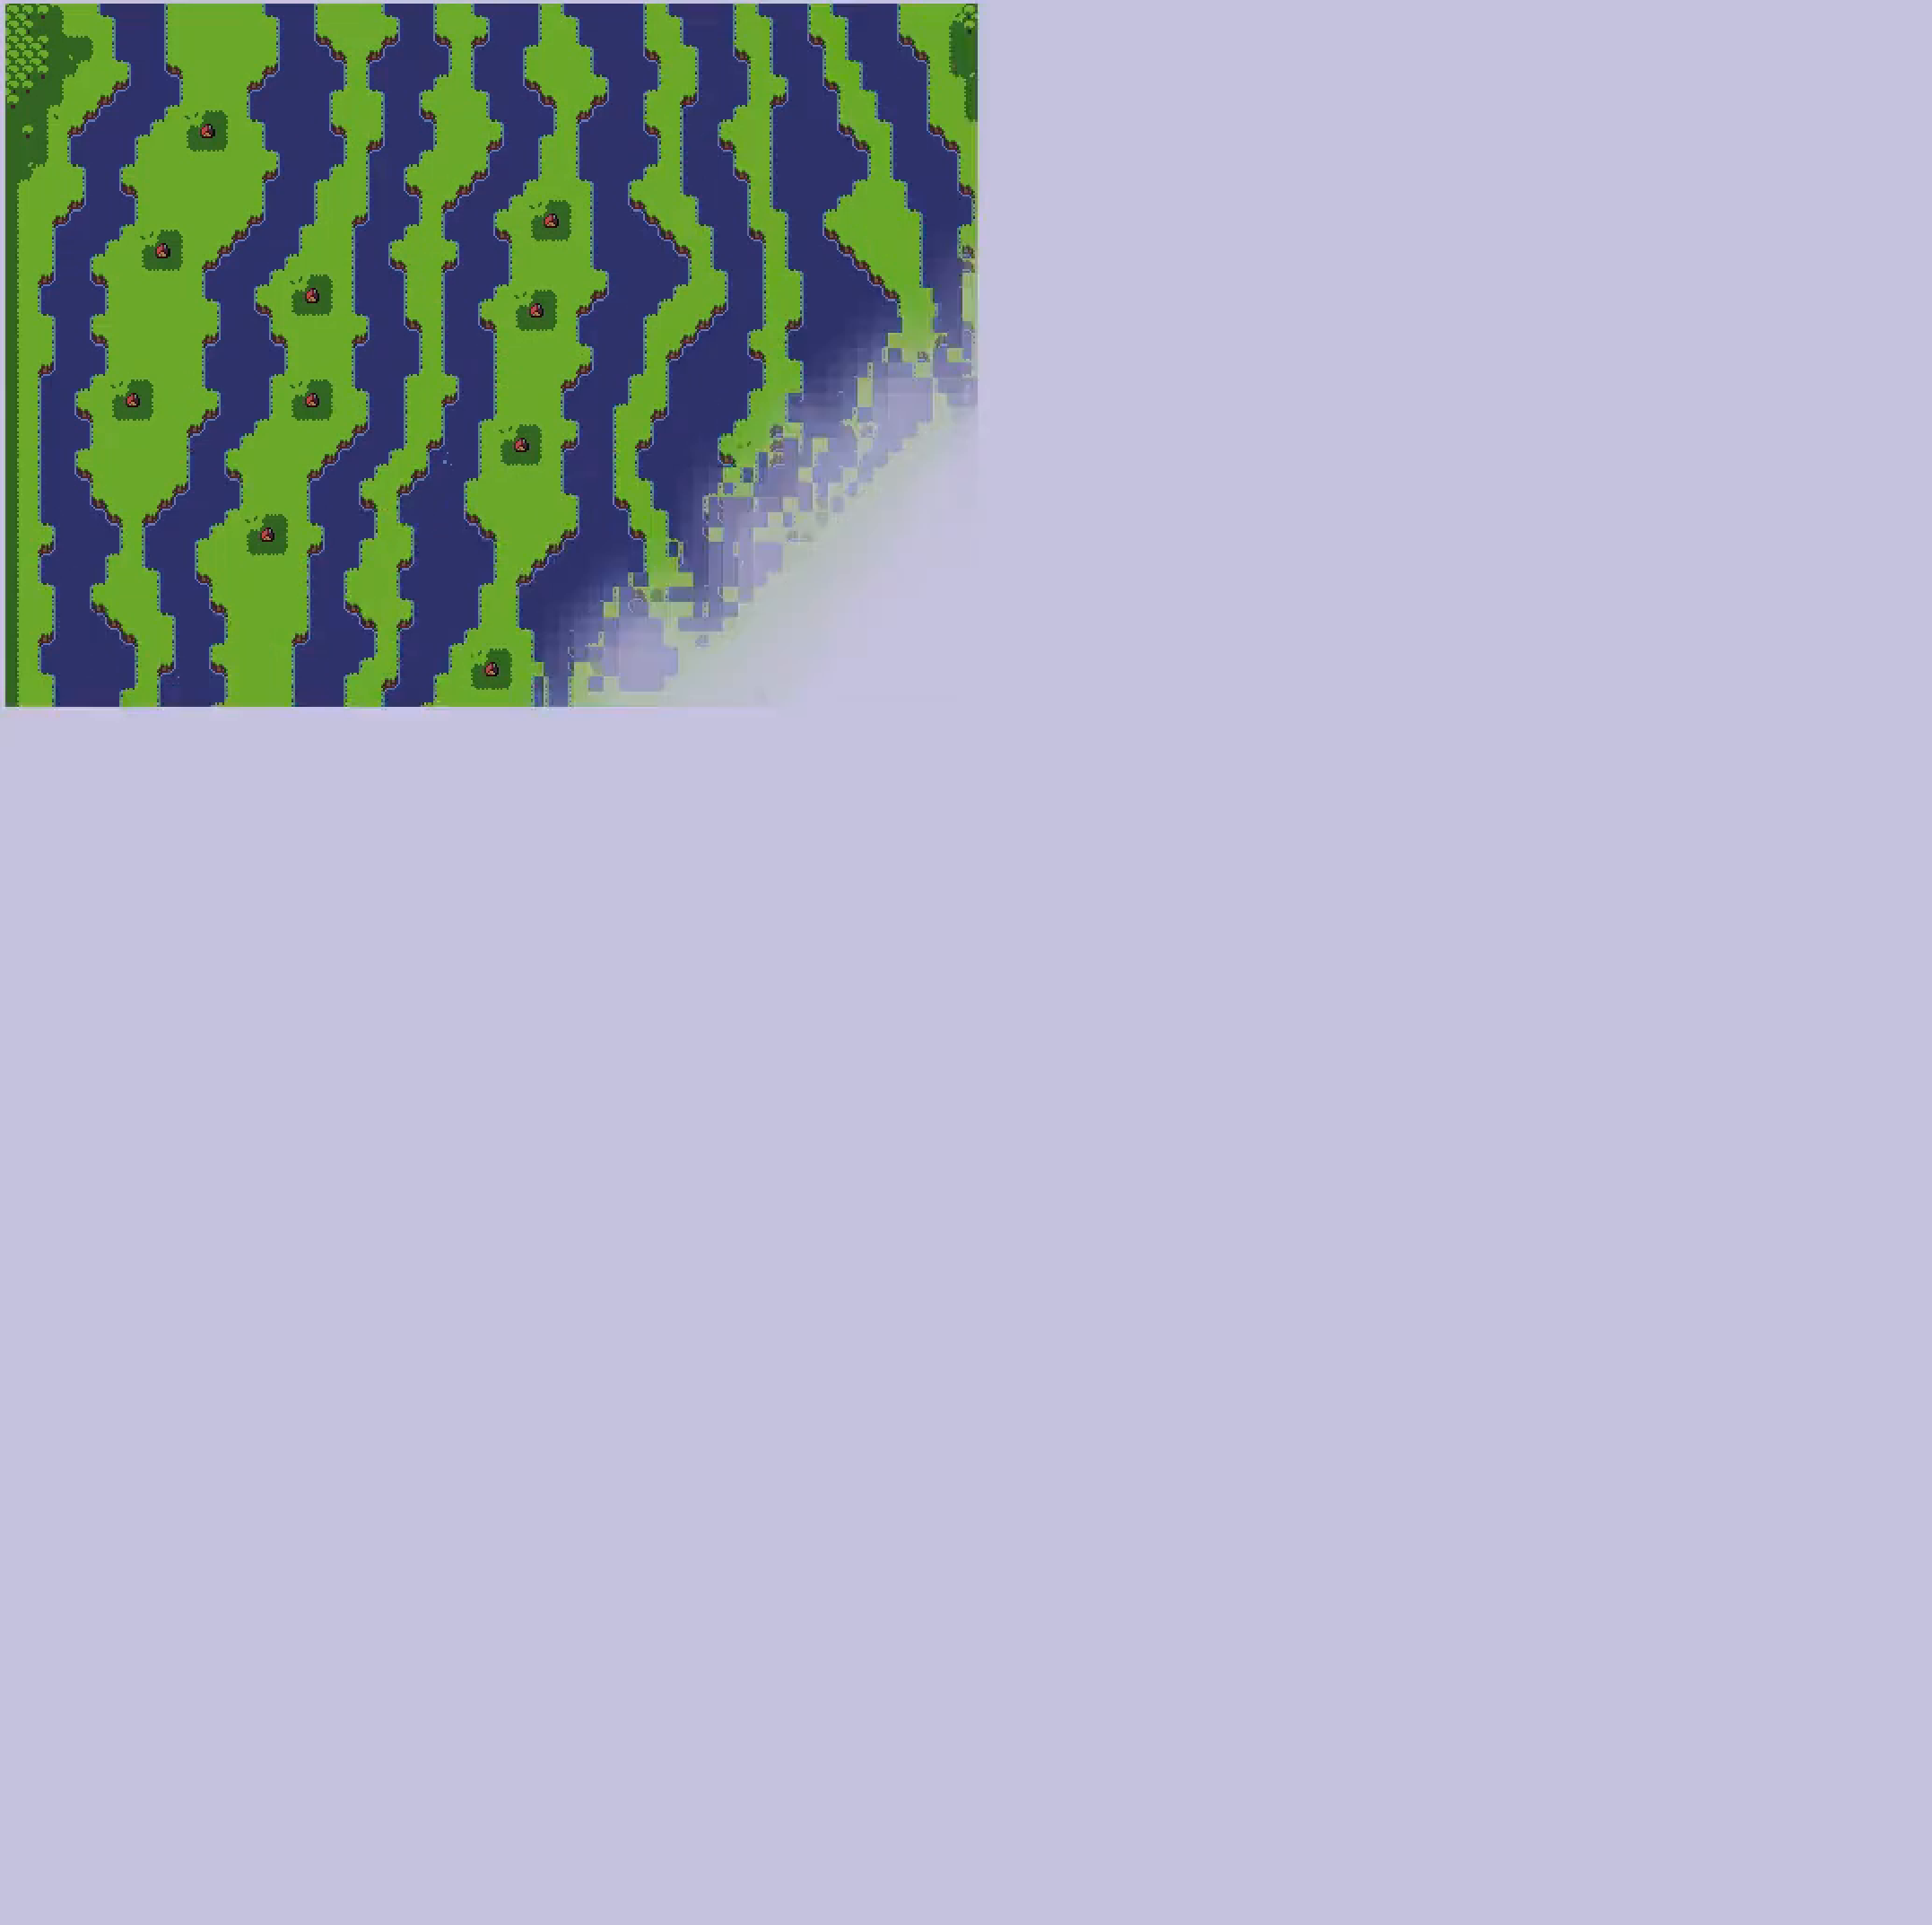
\includegraphics[width=\textwidth]{img/fm_0006.pdf}
%    \end{figure}
%  \end{frame}
%

  %\section{Highlighted Runs}

  \begin{frame}[fragile]{Algorithm}
    \begin{figure}
      \textit{Pill Mortal} Tile Set

      \movie[width=6cm,height=6cm,poster,autostart,repeat]{}{vid/pm_w.mp4}
    \end{figure}
  \end{frame}


%  \begin{frame}[fragile]{Highlighted Runs}
%    \begin{figure}
%      LUNARSIGNAL's \textit{Overhead Action} \\ \textit{RPG Overworld} Tile Set (x10)
%      \movie[width=6cm,height=6cm,poster,autostart,repeat]{}{vid/oarpgo_x10_w.mp4}
%    \end{figure}
%  \end{frame}

%  \begin{frame}[fragile]{Highlighted Runs}
%    \begin{figure}
%      0x72's \textit{Two Bit Micro Metroidvania} Tile Set (x10)
%      \movie[width=6cm,height=6cm,poster,autostart,repeat]{}{vid/2bmmv_x10_w.mp4}
%    \end{figure}
%  \end{frame}

%  \begin{frame}[fragile]{Highlighted Runs}
%    \begin{figure}
%      Kingel's \textit{Minirogue} Tile Set (x10)
%      \movie[width=6cm,height=6cm,poster,autostart,repeat]{}{vid/minirogue_x10_w.mp4}
%    \end{figure}
%  \end{frame}

  %\section{Conclusion}

  \begin{frame}[fragile]{Conclusion}
    Punch Out Model Synthesis (POMS) as an alternative when large models with minimal setup restrictions are wanted
    and resource limits are a concern.
  \end{frame}

  \begin{frame}[fragile]{Conclusion}
    CBTG algorithms are good at maintaining local consistency but are bad at resolving global constraints \\
    \hfill \\
    Weak global constraints (path connections, etc.) confound POMS (and other CBTG algorithms) \\
  \end{frame}

  \begin{frame}[fragile]{fin}
    \begin{center}\url{https://zzyzek.github.io}\end{center}
    \hfill \\
    \begin{center}\url{https://github.com/zzyzek/PunchOutModelSynthesis}\end{center}
    \hfill \\
    \begin{center}\small\url{https://zzyzek.github.io/PunchOutModelSynthesisWebDemo/}\end{center}
    \hfill \\
    \begin{center}Thanks!\end{center}
  \end{frame}

  \appendix

  \begin{frame}[fragile]{Auxiliary Slides}
    Automatic Tile Generation \\
    \url{https://zzyzek.github.io/TileRuleHighlighter/}
    \begin{columns}[T,onlytextwidth]
      \column{0.5\textwidth}
        \begin{block}{Rule Graph (Forest Micro)}
          \begin{figure}
            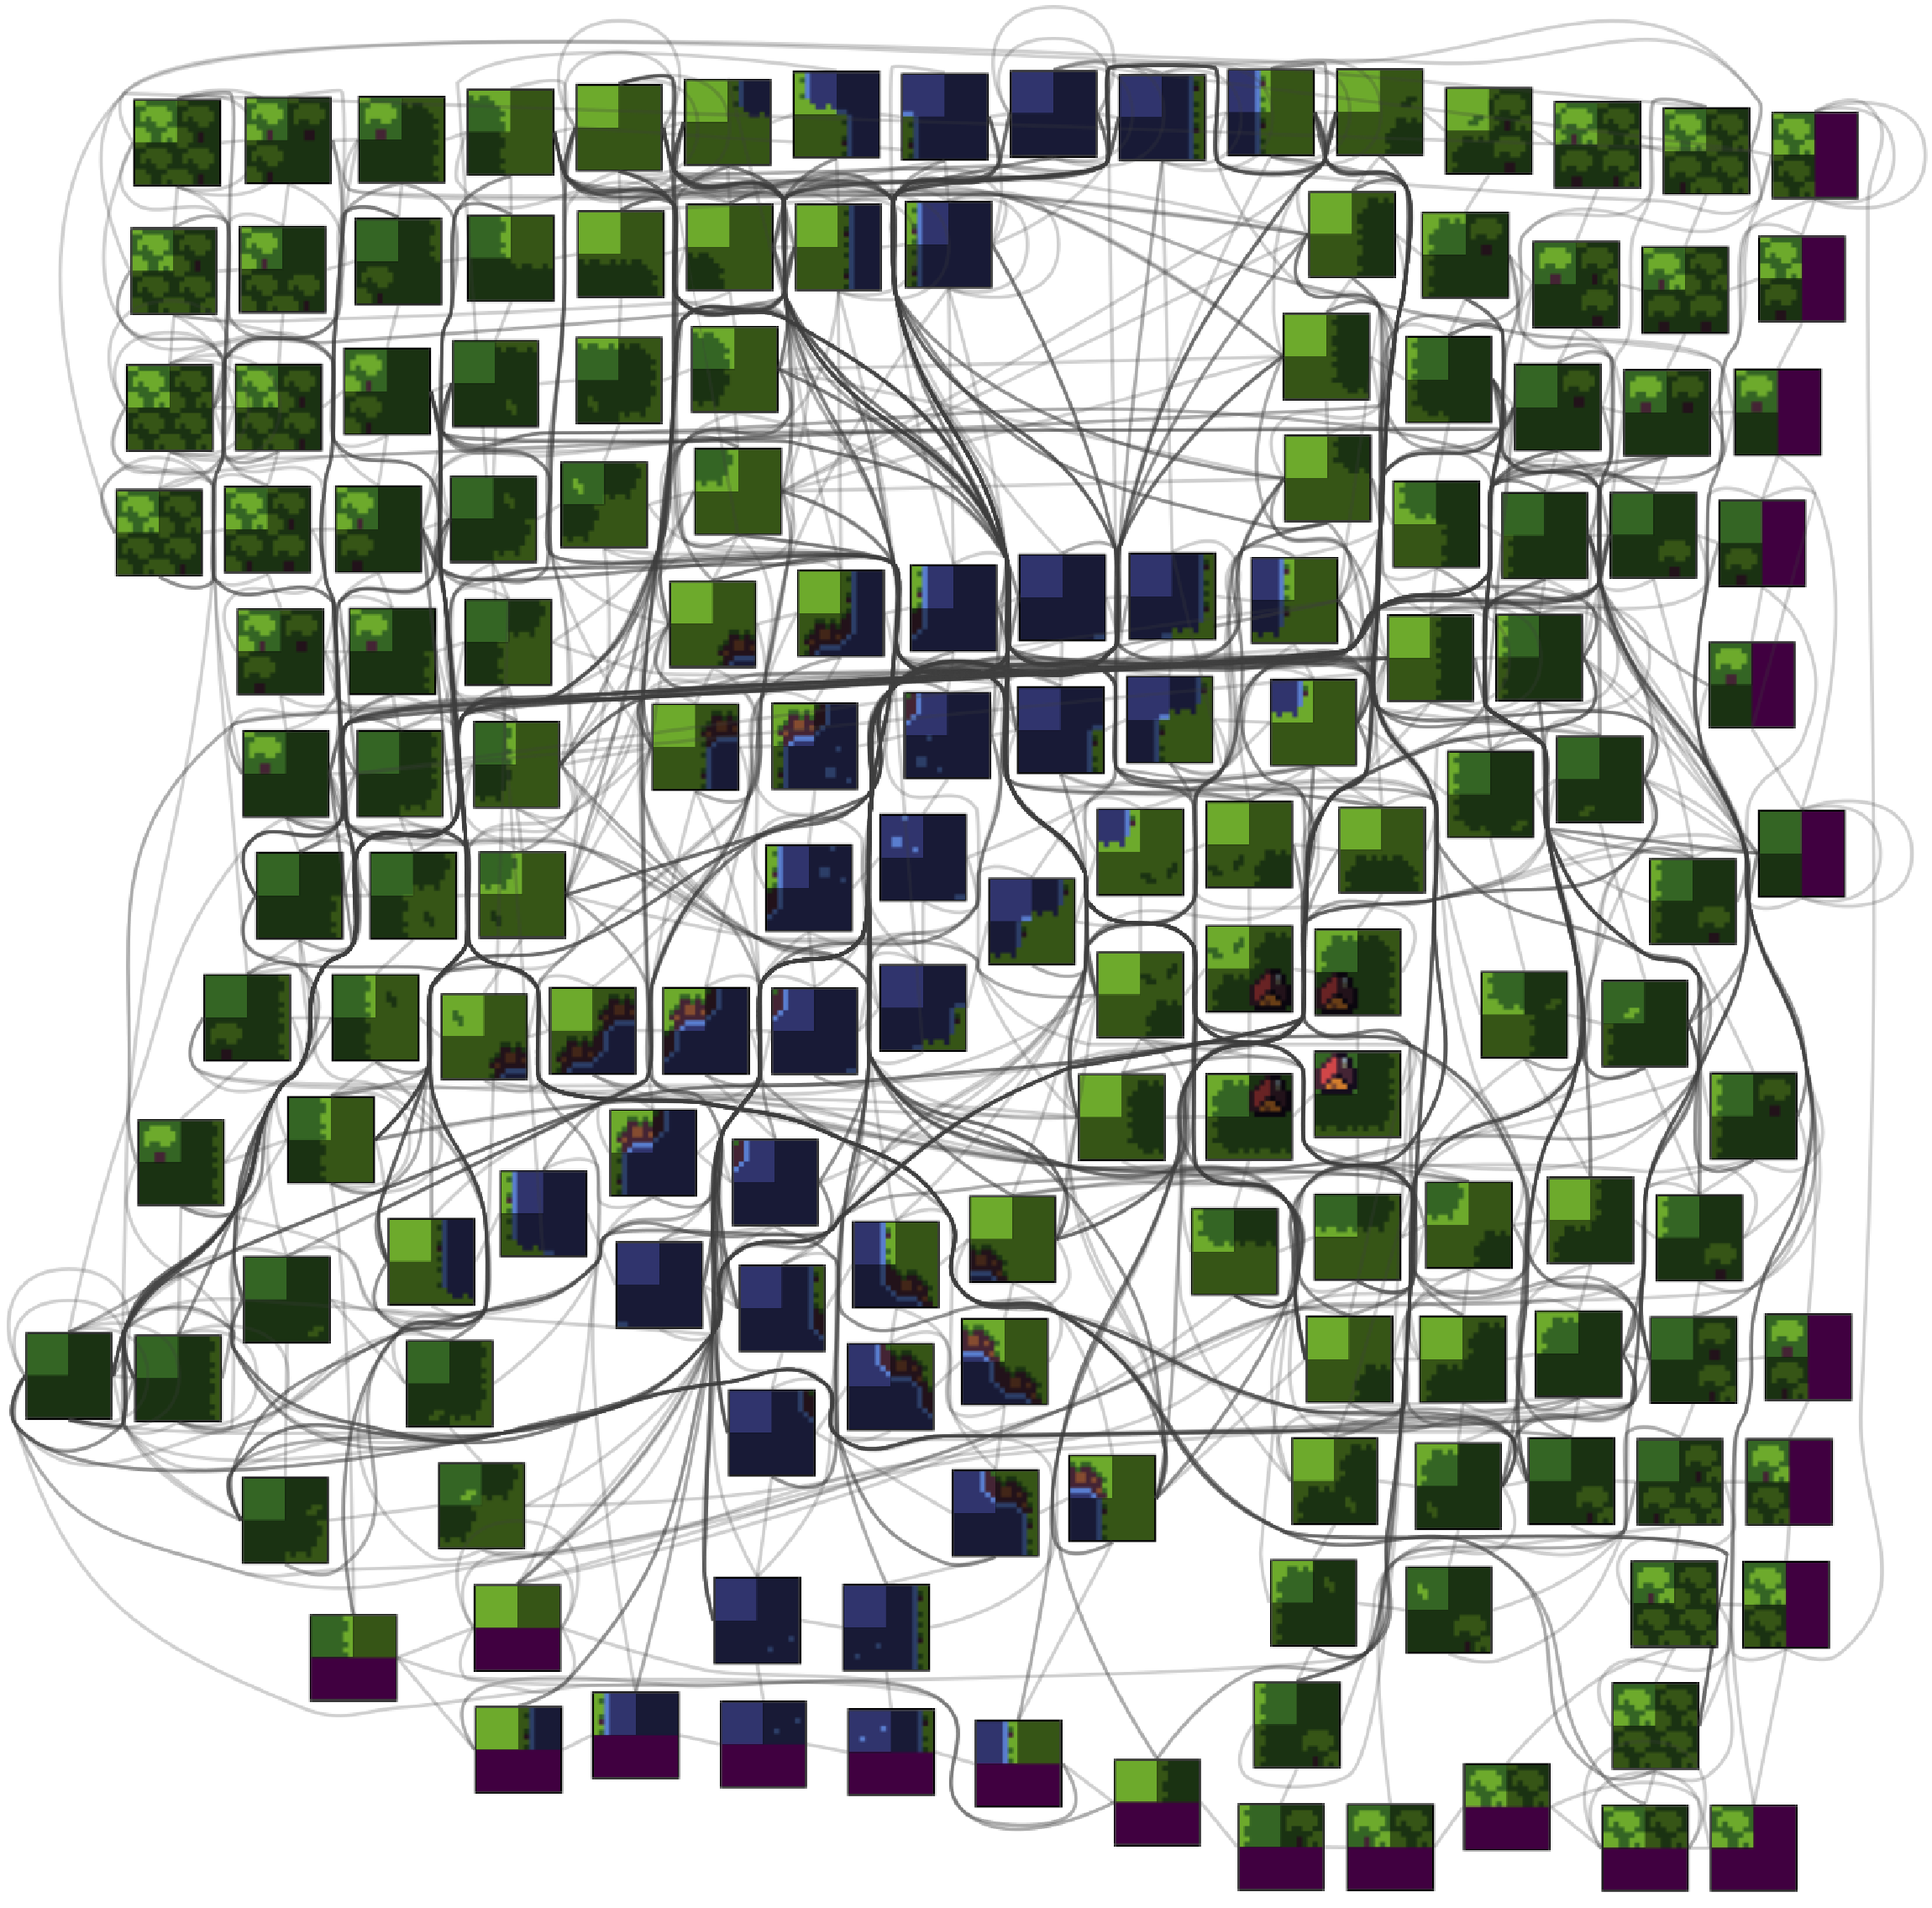
\includegraphics[width=0.7\textwidth]{img/forestmicro_rule_grid_tb.pdf}
          \end{figure}
        \end{block}
      \column{0.5\textwidth}
        \begin{block}{Rule Highlighter}
          \begin{figure}
            %\movie[width=6cm,height=6cm,poster,autostart,repeat]{}{vid/fm_rule_anim.mp4}
            %\movie[width=5cm,height=2.85cm,poster,autostart,repeat]{}{vid/fm_rule_anim.mp4}
            \movie[width=6cm,height=3.4cm,poster,autostart,repeat]{}{vid/fm_rule_anim.mp4}
          \end{figure}
        \end{block}
    \end{columns}

  \end{frame}


  \begin{frame}[fragile]{Highlighted Runs}
    \begin{figure}
      LUNARSIGNAL's \textit{Overhead Action} \\ \textit{RPG Overworld} Tile Set (x10)
      \movie[width=6cm,height=6cm,poster,autostart,repeat]{}{vid/oarpgo_x10_w.mp4}
    \end{figure}
  \end{frame}

  \begin{frame}[fragile]{Highlighted Runs}
    \begin{figure}
      0x72's \textit{Two Bit Micro Metroidvania} Tile Set (x10)
      \movie[width=6cm,height=6cm,poster,autostart,repeat]{}{vid/2bmmv_x10_w.mp4}
    \end{figure}
  \end{frame}

  \begin{frame}[fragile]{Highlighted Runs}
    \begin{figure}
      Kingel's \textit{Minirogue} Tile Set (x10)
      \movie[width=6cm,height=6cm,poster,autostart,repeat]{}{vid/minirogue_x10_w.mp4}
    \end{figure}
  \end{frame}


  \begin{frame}[fragile]{Auxiliary Slides}
    \begin{itemize}
      \item Bitter lesson includes learning \textit{and} search
      \item Trade off between resources used to learn vs. resources used for run time search
      \item "Parables of the Power of Planning in AI" by Noam Brown (\url{https://www.youtube.com/watch?v=eaAonE58sLU})
    \end{itemize}
  \end{frame}

  \begin{frame}[fragile]{Auxiliary Slides}
    Other Problems

    \begin{itemize}
      \item Salad
      \item Oatmeal
      \item Global Cohesion/(weak) Global Constraints
    \end{itemize}
  \end{frame}


  \begin{frame}[fragile]{Auxiliary Slides}
    Potential Future Work

    \begin{itemize}
      \item Spectral Graph Decomposition methods for automatic biome detection
      \item AC4 speedups via templates
      \item Weak global constraints
    \end{itemize}
  \end{frame}


\end{document}
